\chapter{Histological grade prediction via automatic liver tumors segmentation}\label{contributions_xp}


In this chapter we present the experimental results of our work.
We first describe more precisely the different key concepts 
to be implemented such as the cascaded architecture or the 
incorporation of the multiphase images.
We then expose our semantic segmentation experiments where 
the best performances were obtained by stacking several 
specialized networks with dynamic contrast-enhanced images as input.
After validating the value brought by our semantic segmentation architecture
to provide additional annotations in the case of weakly annotated datasets, 
we describe our \ac{dlr} pipeline which incorporated the relevant semantic imaging features 
for the prediction of the histological grade.

\section{Semantic segmentation applied to the study of HCC}

As explained previously, state-of-the-art deep learning techniques allow
modern hardware to perform automatic segmentation of both the liver and
its structures with a precision close to the one obtained by the experts
themselves.
In this section, we will first describe the implemented
networks and the different used datasets, before presenting the experiments.
%As described previously, no real consensus was made regarding the
%design of the \ac{dl}-related semantic segmentation studies, so we decided to
%launch several experiments on selected datasets to determine the impact
%of the training strategies on the performances of the networks.
After selecting an optimal set of hyperparameters, we evaluated the
advantages brought by a cascaded architecture, and the way to implement
it, before describing the way to incorporate the multiphase information
in our architecture.
The results and the conclusions of this work were presented in the
literature \cite{Ouhmich2019}.


\subsection{Motivations}

We implemented different architectures to validate the hypothesis that
current deep networks can perform automatic delineation of both the
liver and its tumors. 
The wash-in wash-out being an important characteristic of the tumor, we decided to design an architecture that will try to extract features encoding this specific information. We wanted to prove that incorporating the dynamic information through the use of contrast-enhanced images can improve the performances of the network, therefore, we compared results obtained using single and multi-phase networks. \\
We built several architectures to confirm that the cascaded approach corresponds to the best paradigm when dealing with small multiphase datasets.
Finally, we proved the ability of our cascaded architecture to provide additional annotations in weakly annotated datasets.\\
It it worth noting that we are the first to automatically 
delineate \ac{hcc} on multiphase \ac{ct} images using a \ac{dl} architecture, and that features computed by the our architecture will further be used in a radiomics purpose to predict the histological grade.



\subsection{Cascaded architecture}

Even though no consensus was made regarding existing methods, we noticed that
several studies implemented a sequential pipeline that can be modeled as
cascaded architecture. The cascade consists in several networks trained
to perform a specific simpler task, and that are sequentially connected, to
provide a final annotation map. In our case, the goal is the
segmentation of the liver and its internal structures with the
differentiation between parenchyma, and both the active and the necrotic
parts of the hepatic tumor.
Our cascade will consequently be composed of 3 networks, as depicted
in the figure \ref{CARS_Cascade}. The first one will be specialized to segment the liver in
abdominal axial slices, the second will delineate the contours of the
tumor in the predicted liver \ac{roi}, whereas the final one will
differentiate between active and necrotic parts within the obtained
tumor \ac{roi} \cite{Ouhmich2019}.
Each one of the given networks will share the same \emph{U-Net}
architecture.

\begin{figure}[th!]
	\centering
	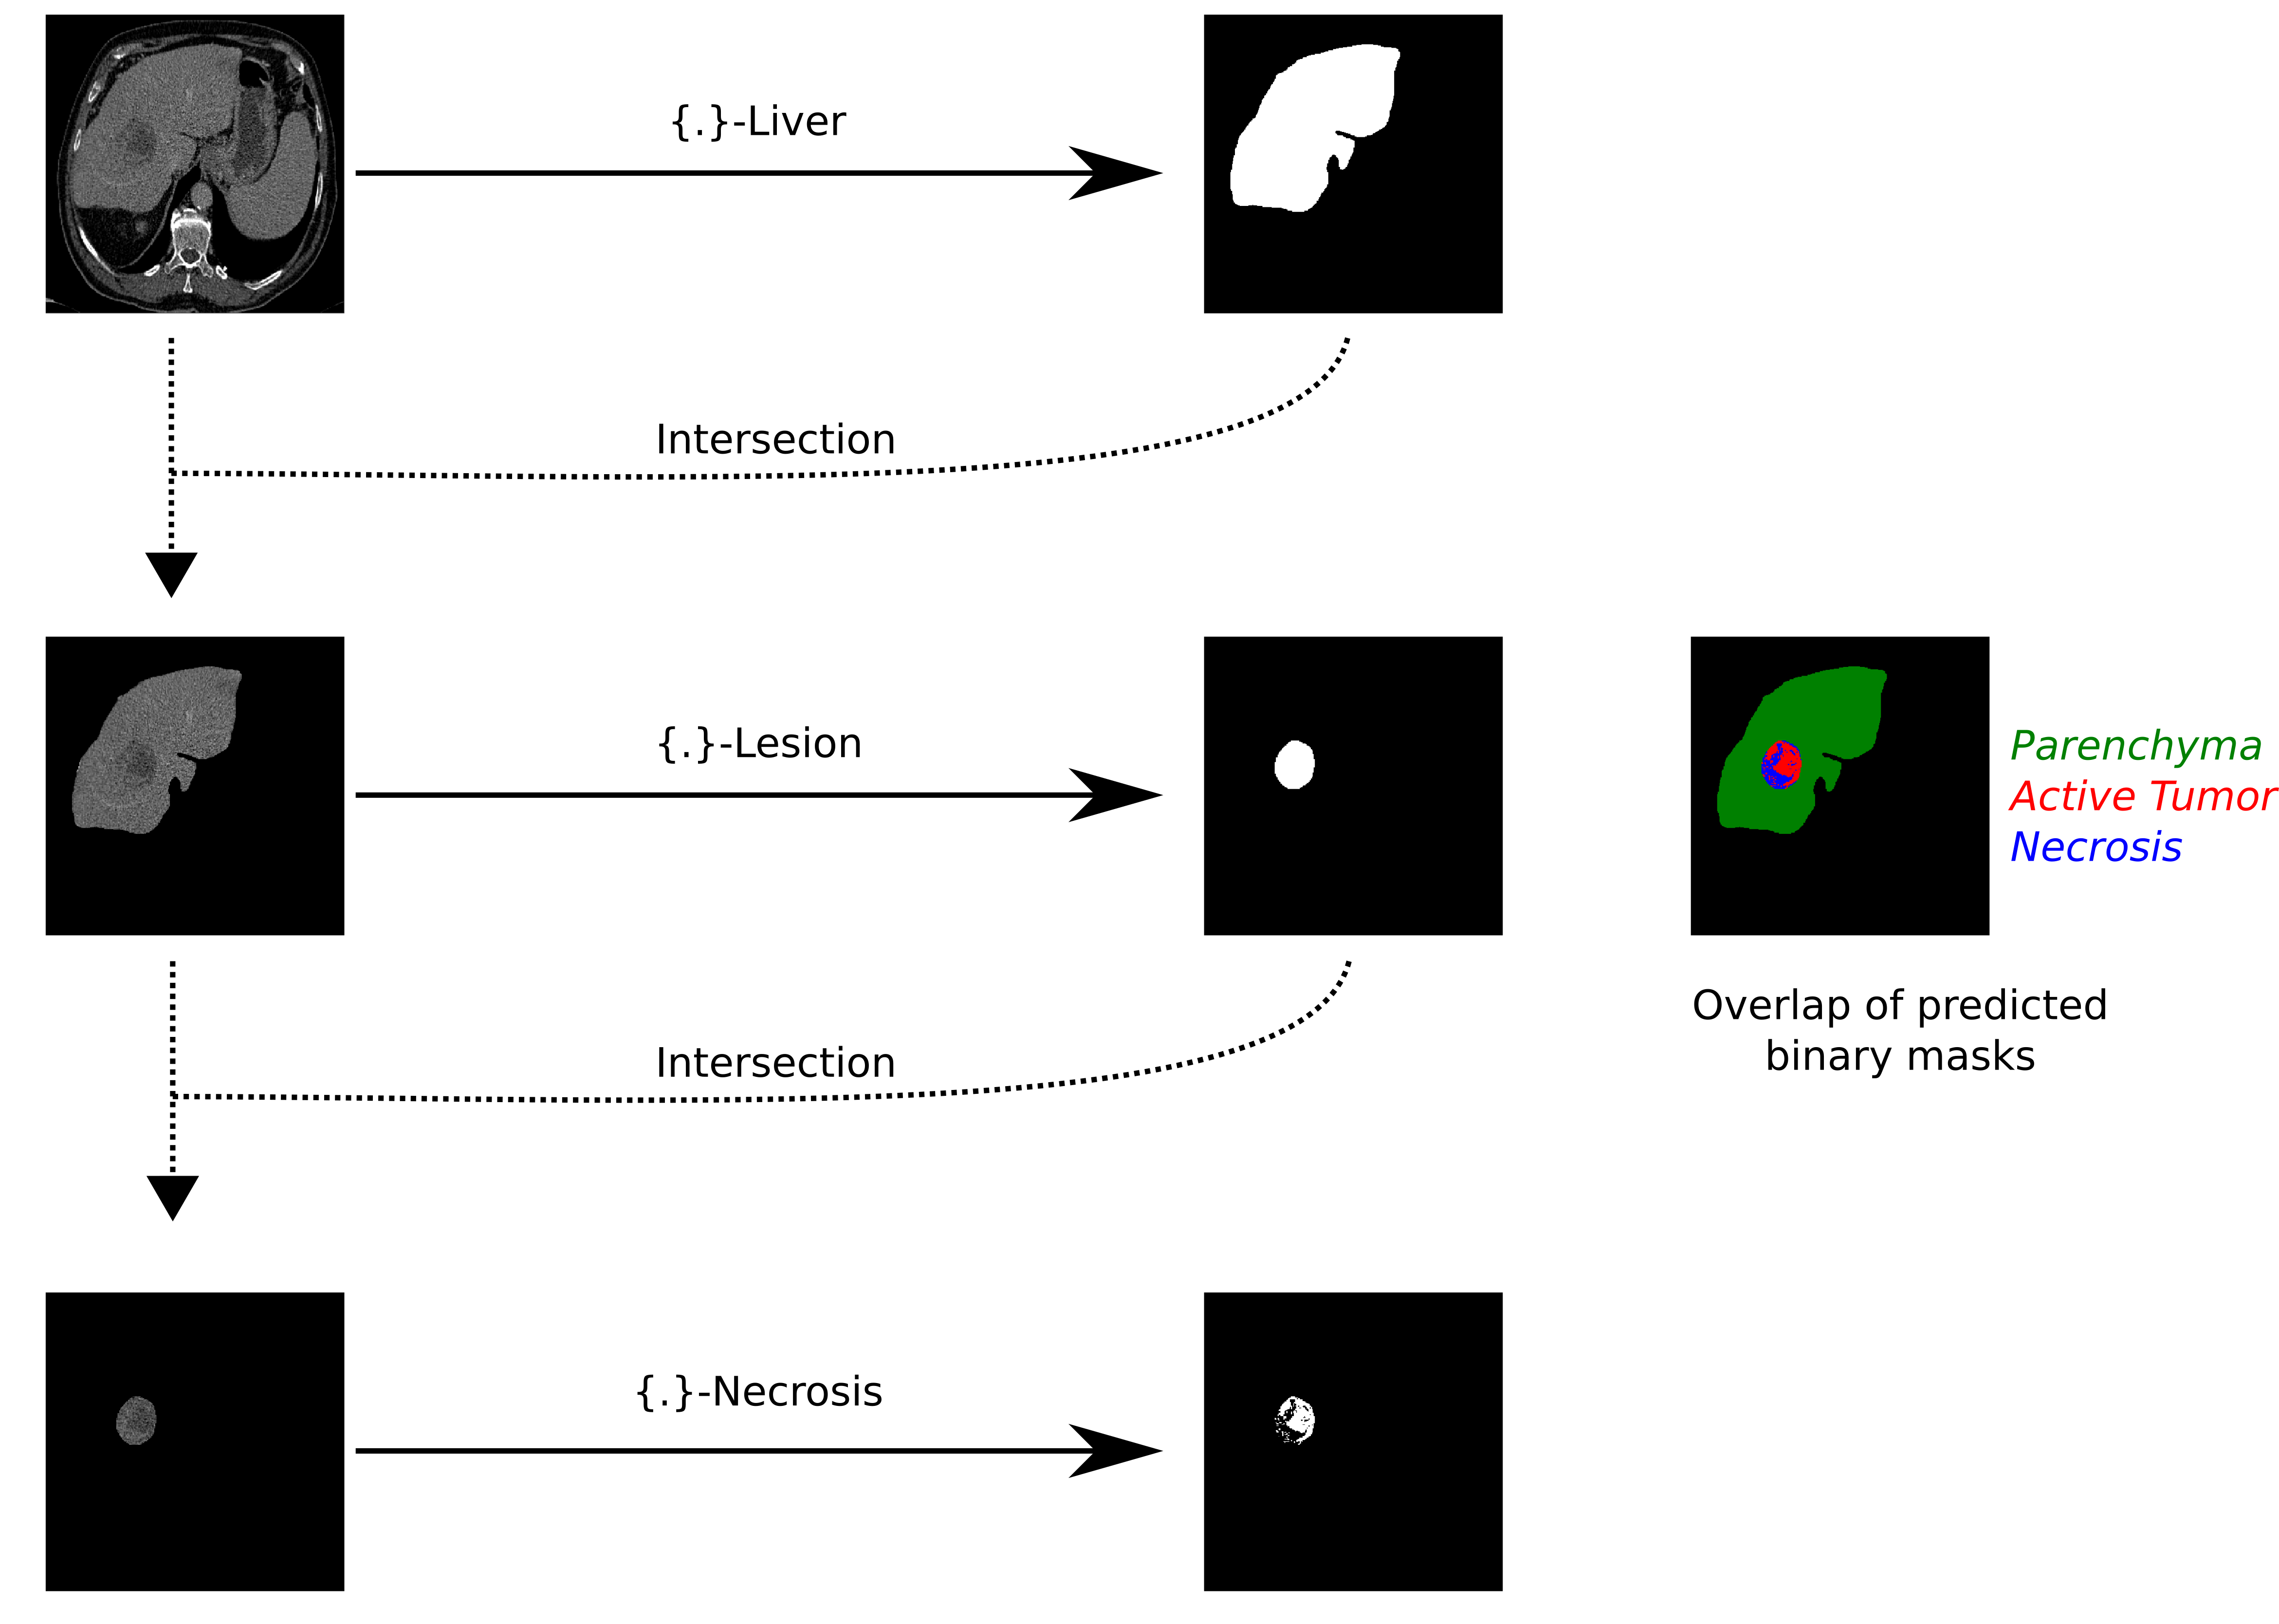
\includegraphics[width=0.7\linewidth]{../SemanticSeg/images/Cascade2}
	\caption{Cascaded network: The first network takes as input a \ac{ct} image and segments the liver. The resulting segmentation map is used to remove non-liver pixels in the input data of the second network which performs the segmentation of lesions. The last network segments the necrosis within the lesions. The three binary masks are combined in the final segmentation map.}
	\label{CARS_Cascade}
\end{figure}


\subsection{U-Net network}

As a basis architecture, we have decided to implement \emph{U-Net} like
networks because it has been previously used for the semantic
segmentation task, and has proven to give good results even with a
small number of training samples. \\
The original \emph{U-Net} architecture was developed by Ronneberger et
al. \cite{Ronneberger2015} and initially designed for the
delineation of cells in microscopic images. As detailed previously, the
network can be divided into two subparts, a contraction one where the
information contained within the images is compressed, through the
extraction of high to low level features, and a decoding part where the
compressed information is used to reconstruct a high resolution
segmentation. The architecture was initially composed of 19
convolutional layers, with a rectified linear unit function as
activation. The input image had an initial size of $ 512\times512 $ pixels, and
at each stage of the encoding part, 2 convolutional layers are stacked
with an increased number of filters. The initial pair of convolution
layers used 64 filters each, whereas the final stage of the encoding
stage used 1024 filters. After each pair of convolutional layers, a max
pooling layer is applied to halve the spatial dimension of the features
maps. As a result, a $ 30\times30\times1024 $ features map is produced at the
bottleneck of the network. This representation is then reformatted in
the decoding part to obtain a segmentation map with a size equivalent to
the one of the input image. In order to increase the spatial dimension
of the features maps, Up-Convolutional layers are implemented. It is worth
noting that the number of filters used in each of the pair of
convolutional layers is decreased from the bottleneck to the final layer
of the network. The last convolutional layers will map the obtained
features to the final number of dimensions of the segmentation maps,
which will correspond to the number of classes to predict. The final
layer implements a softmax function, to simulate a prediction of
appartenance to each one of the output class.

In comparison to the original architecture, we have implemented
zero-padding convolutions to preserve the image size and obtain a
segmentation map with the same spatial dimension as the input image. We
conserved the same settings as in the original architecture concerning
the number of filters to use at each stage, starting with a pair of
convolutions of 64 filters each, and reaching a $ 32\times32\times1024 $ features map
in the bottleneck part of the network. \\
The same naming-system as in our study will be used
here \cite{Ouhmich2019}. Single-phase elementary networks will be referred to by both the
input phase and the segmentation target, as an example, \pplfont{\ac{pv}-Lesion} will
refer to the network responsible for the segmentation of the lesion,
with \ac{pv} (Portal Venous) phase images as input. The complete \emph{U-Net}
architecture for this specific elementary network is depicted in the figure \ref{CARS_PV_lesion_Fig}.

\begin{figure}[th!]
	\centering
	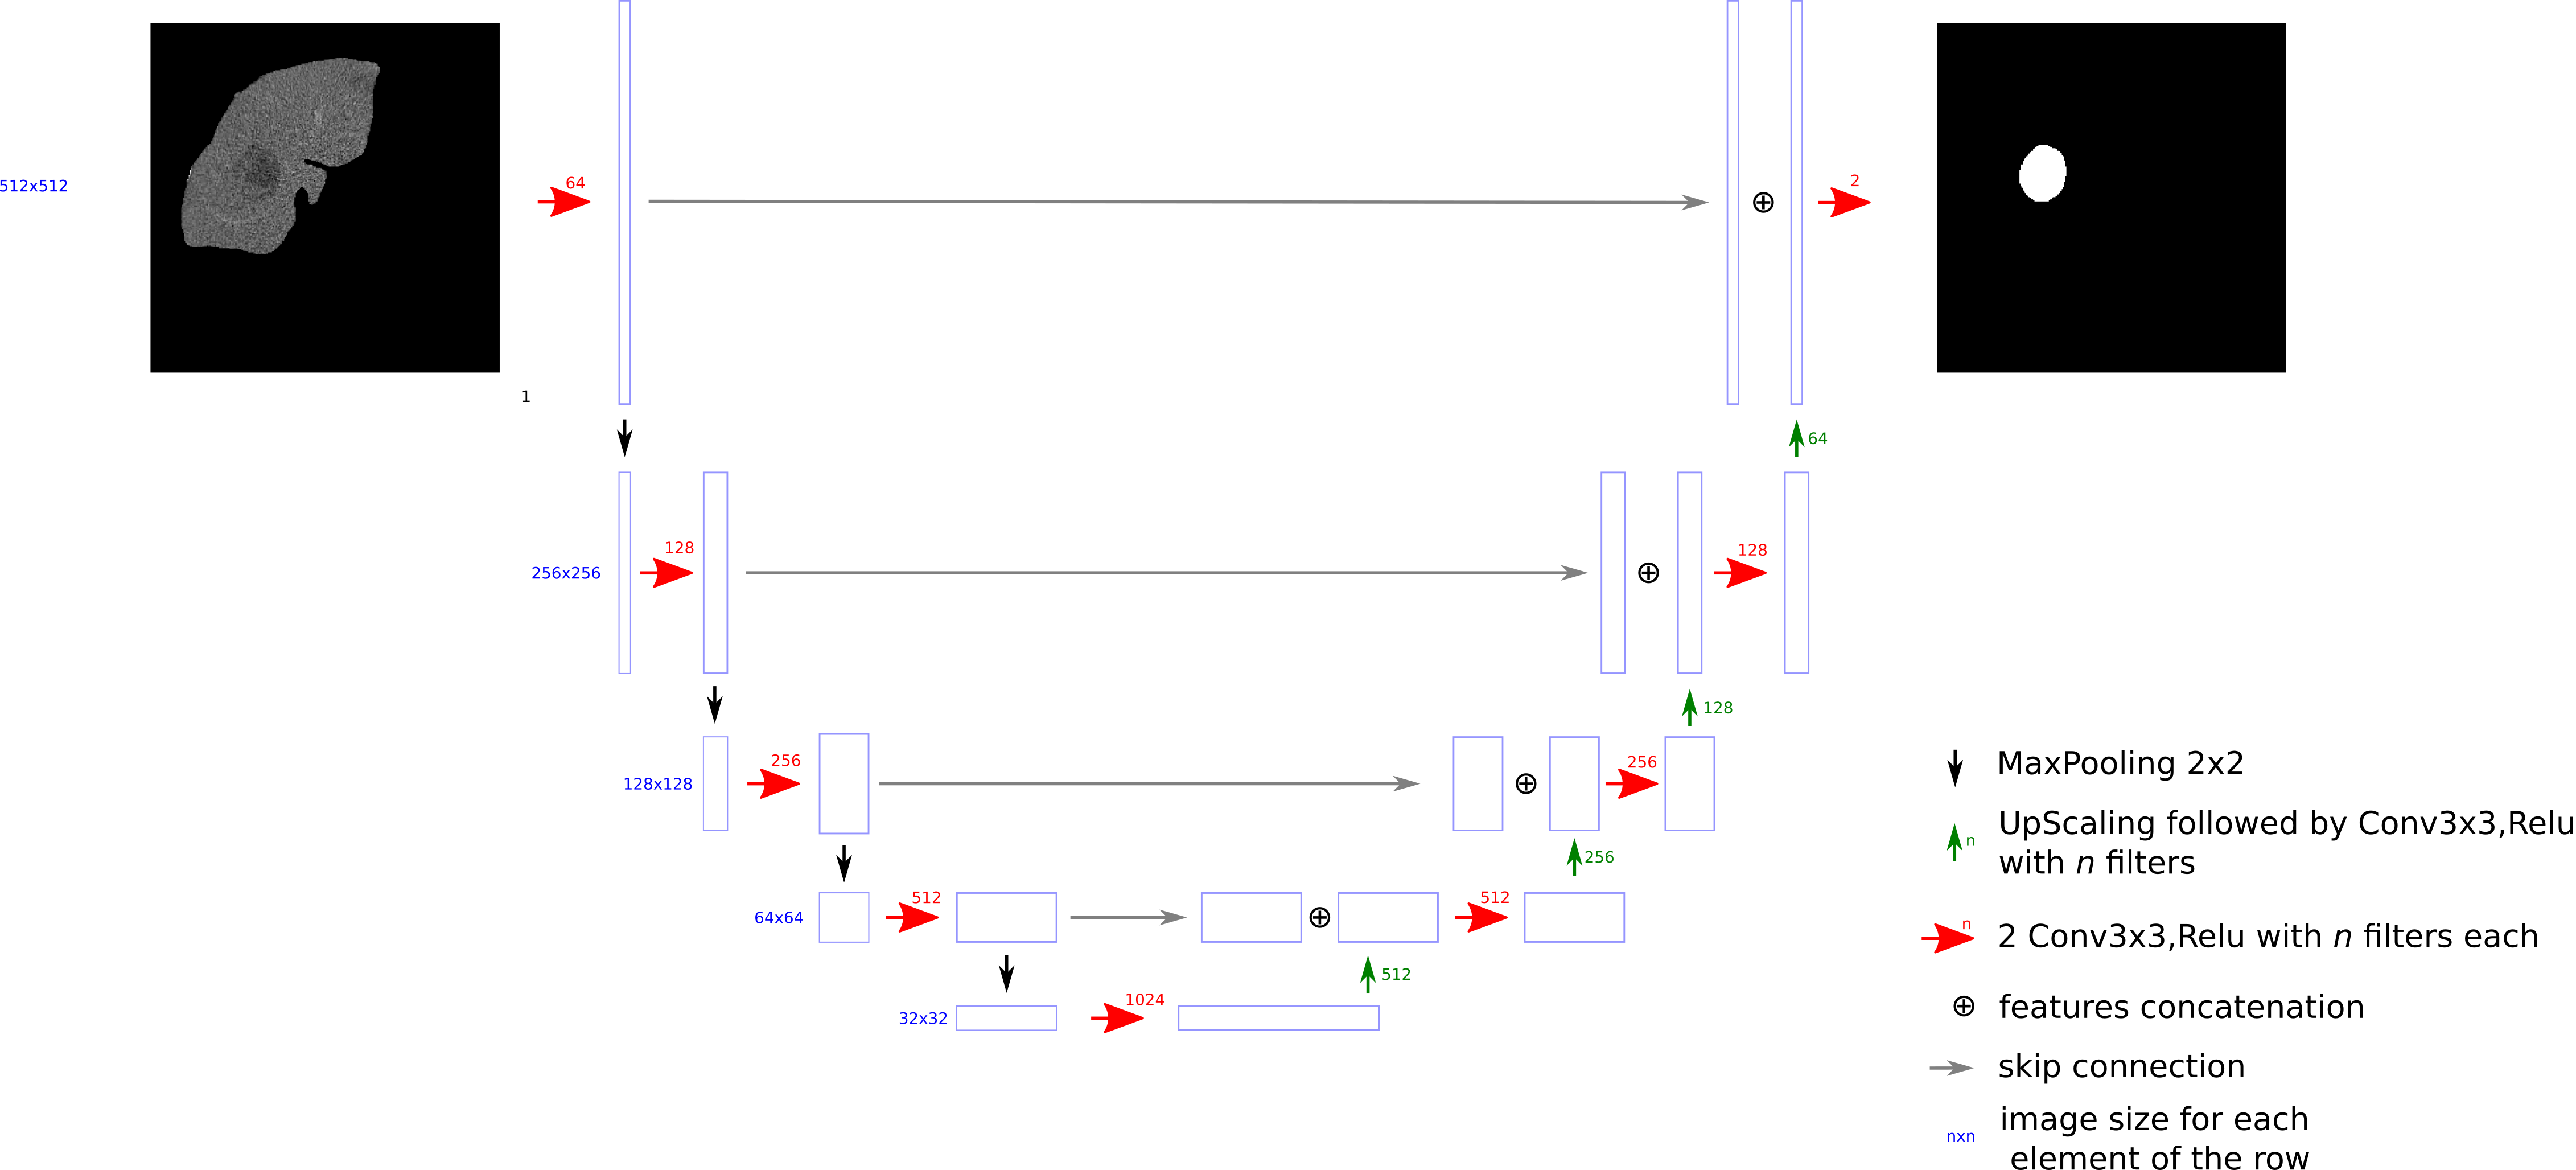
\includegraphics[width=0.9\linewidth]{../SemanticSeg/images/PV_Lesion}
	\caption{\pplfont{\ac{pv}-Lesion} network used to segment lesions within the liver with a \ac{pv} image as input}
	\label{CARS_PV_lesion_Fig}
\end{figure}


In order to evaluate the improvements brought by the cascaded
architecture, we also trained the original \emph{U-Net} architecture to
perform simultaneously the whole internal tissues segmentation task. The
same naming system as previously will be used where ``Full'' corresponds
to the simultaneous segmentation task, thus, \pplfont{AR-Full} will refer to the
network dedicated to the segmentation of both the parenchyma, the active
and the necrotic part of the lesions simultaneously, with AR
images as input. An illustration of the network is given in the figure
\ref{CARS_ArFull_Fig}.

\begin{figure}[th!]
	\centering
	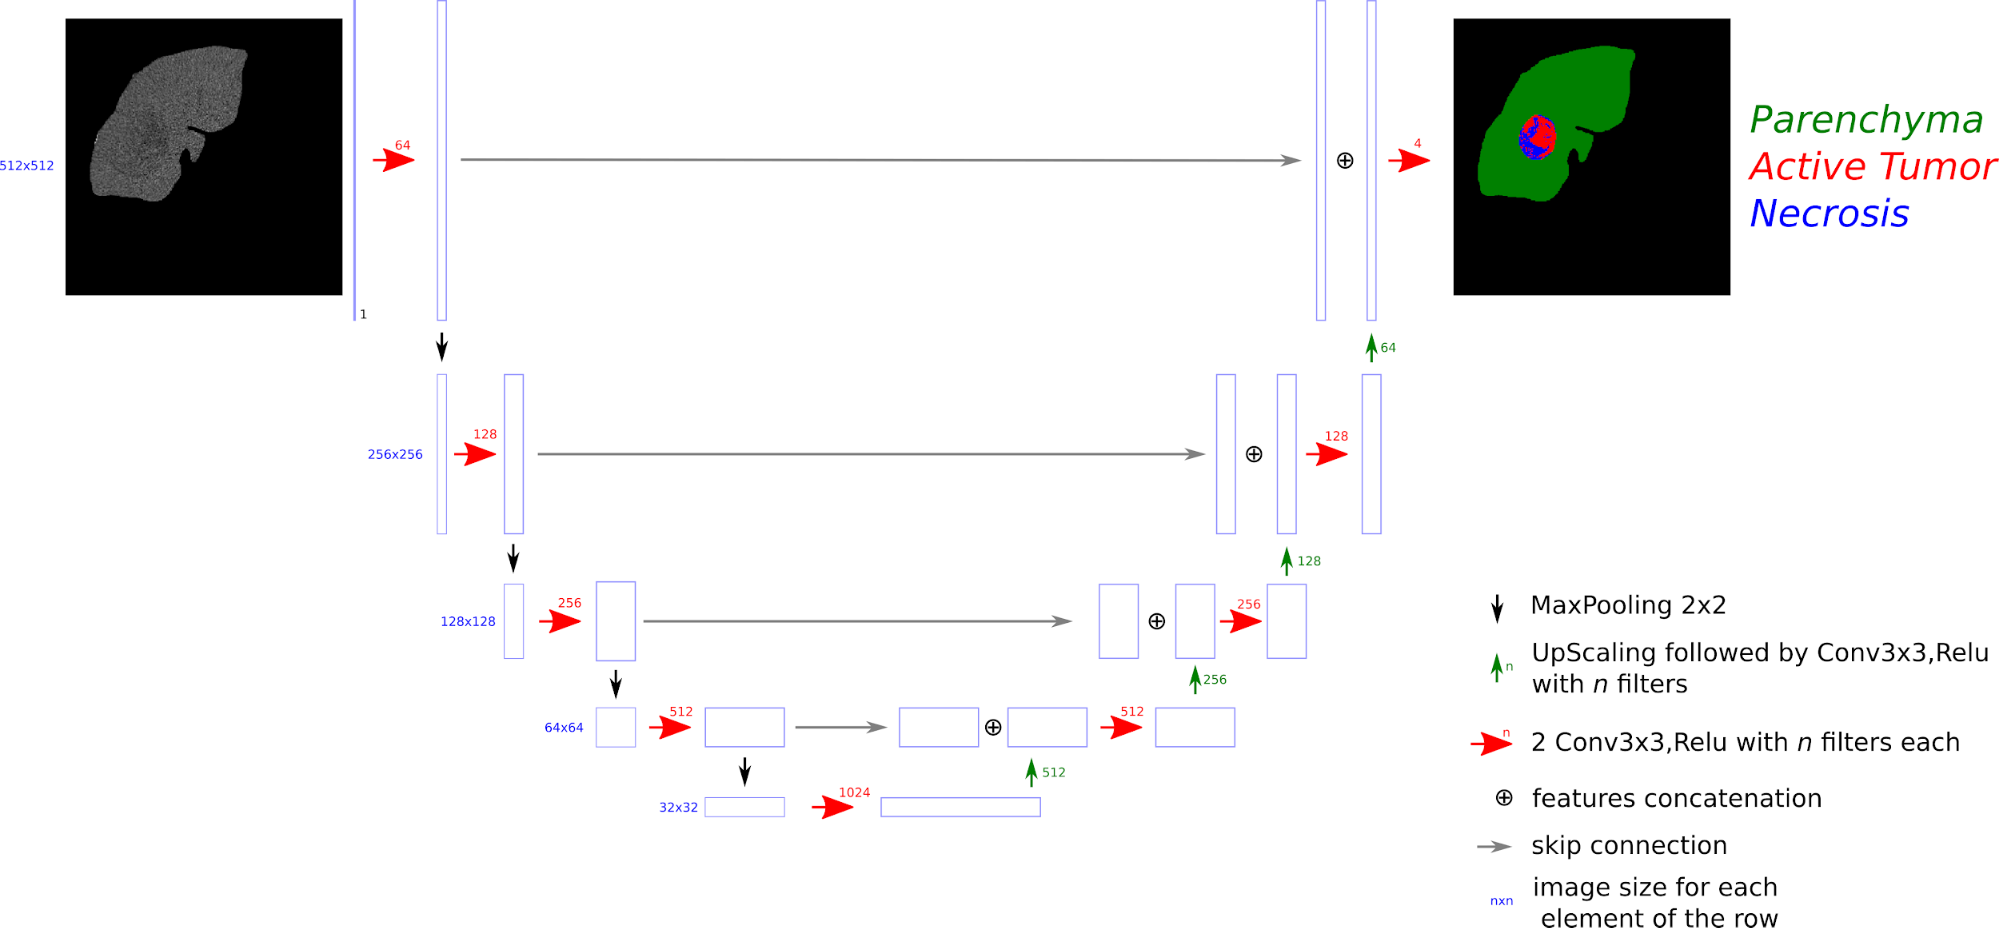
\includegraphics[width=0.9\linewidth]{../SemanticSeg/images/image23}
	\caption{\pplfont{AR-Full} refers to the network trained with AR images as input (values outside the liver are masked), and that outputs a label map, with parenchyma, active and necrotic parts annotated}
	\label{CARS_ArFull_Fig}
\end{figure}


\subsection{Multiphase information}

Only the \ac{ar} and \ac{pv} phases were considered in the
multiphase networks because \ac{nect} phase images do not provide enough
inter-tissue contrast. \\
In order to incorporate the multiphase information in our pipeline, we
investigated 2 different strategies. The first one, referred to as DMP (Dimensional MultiPhase), consists in concatenating both the
AR and \ac{pv} images as input to the network (see figure \ref{CARS_DMP_Full_Fig}).
The second one referred to as MPF (MultiPhase Fusion), consists
in performing both the encoding and the decoding separately for each
phase, before merging the output maps (simple addition on the obtained
features maps), as depicted in the figure \ref{CARS_MPF_Full_Fig}.

\begin{figure}[th!]
	\centering
	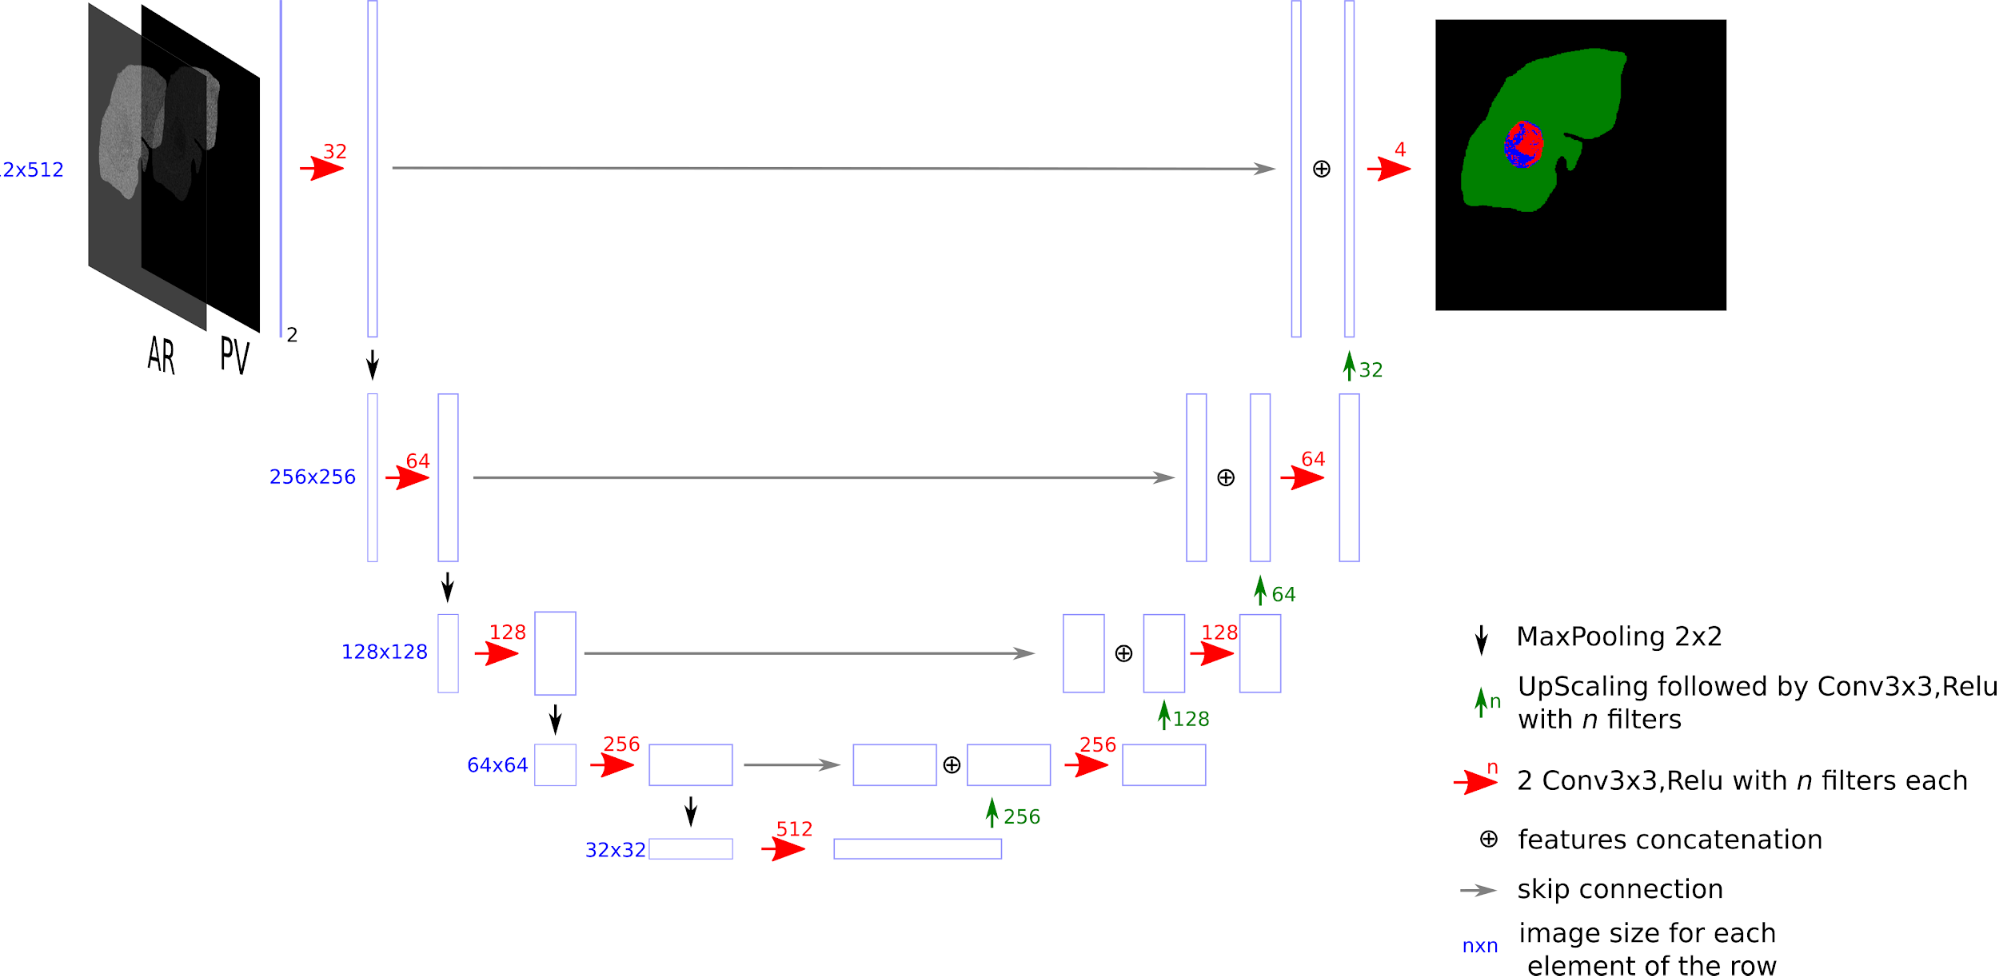
\includegraphics[width=0.9\linewidth]{../SemanticSeg/images/image28}
	\caption{\pplfont{DMP-Full} network that combines the AR and the \ac{pv} images as an input to segment the parenchyma and both the active and the necrotic parts of the lesions. Here, the two channels are considered as features for the first layer}
	\label{CARS_DMP_Full_Fig}
\end{figure}


\begin{figure}[th!]
	\centering
	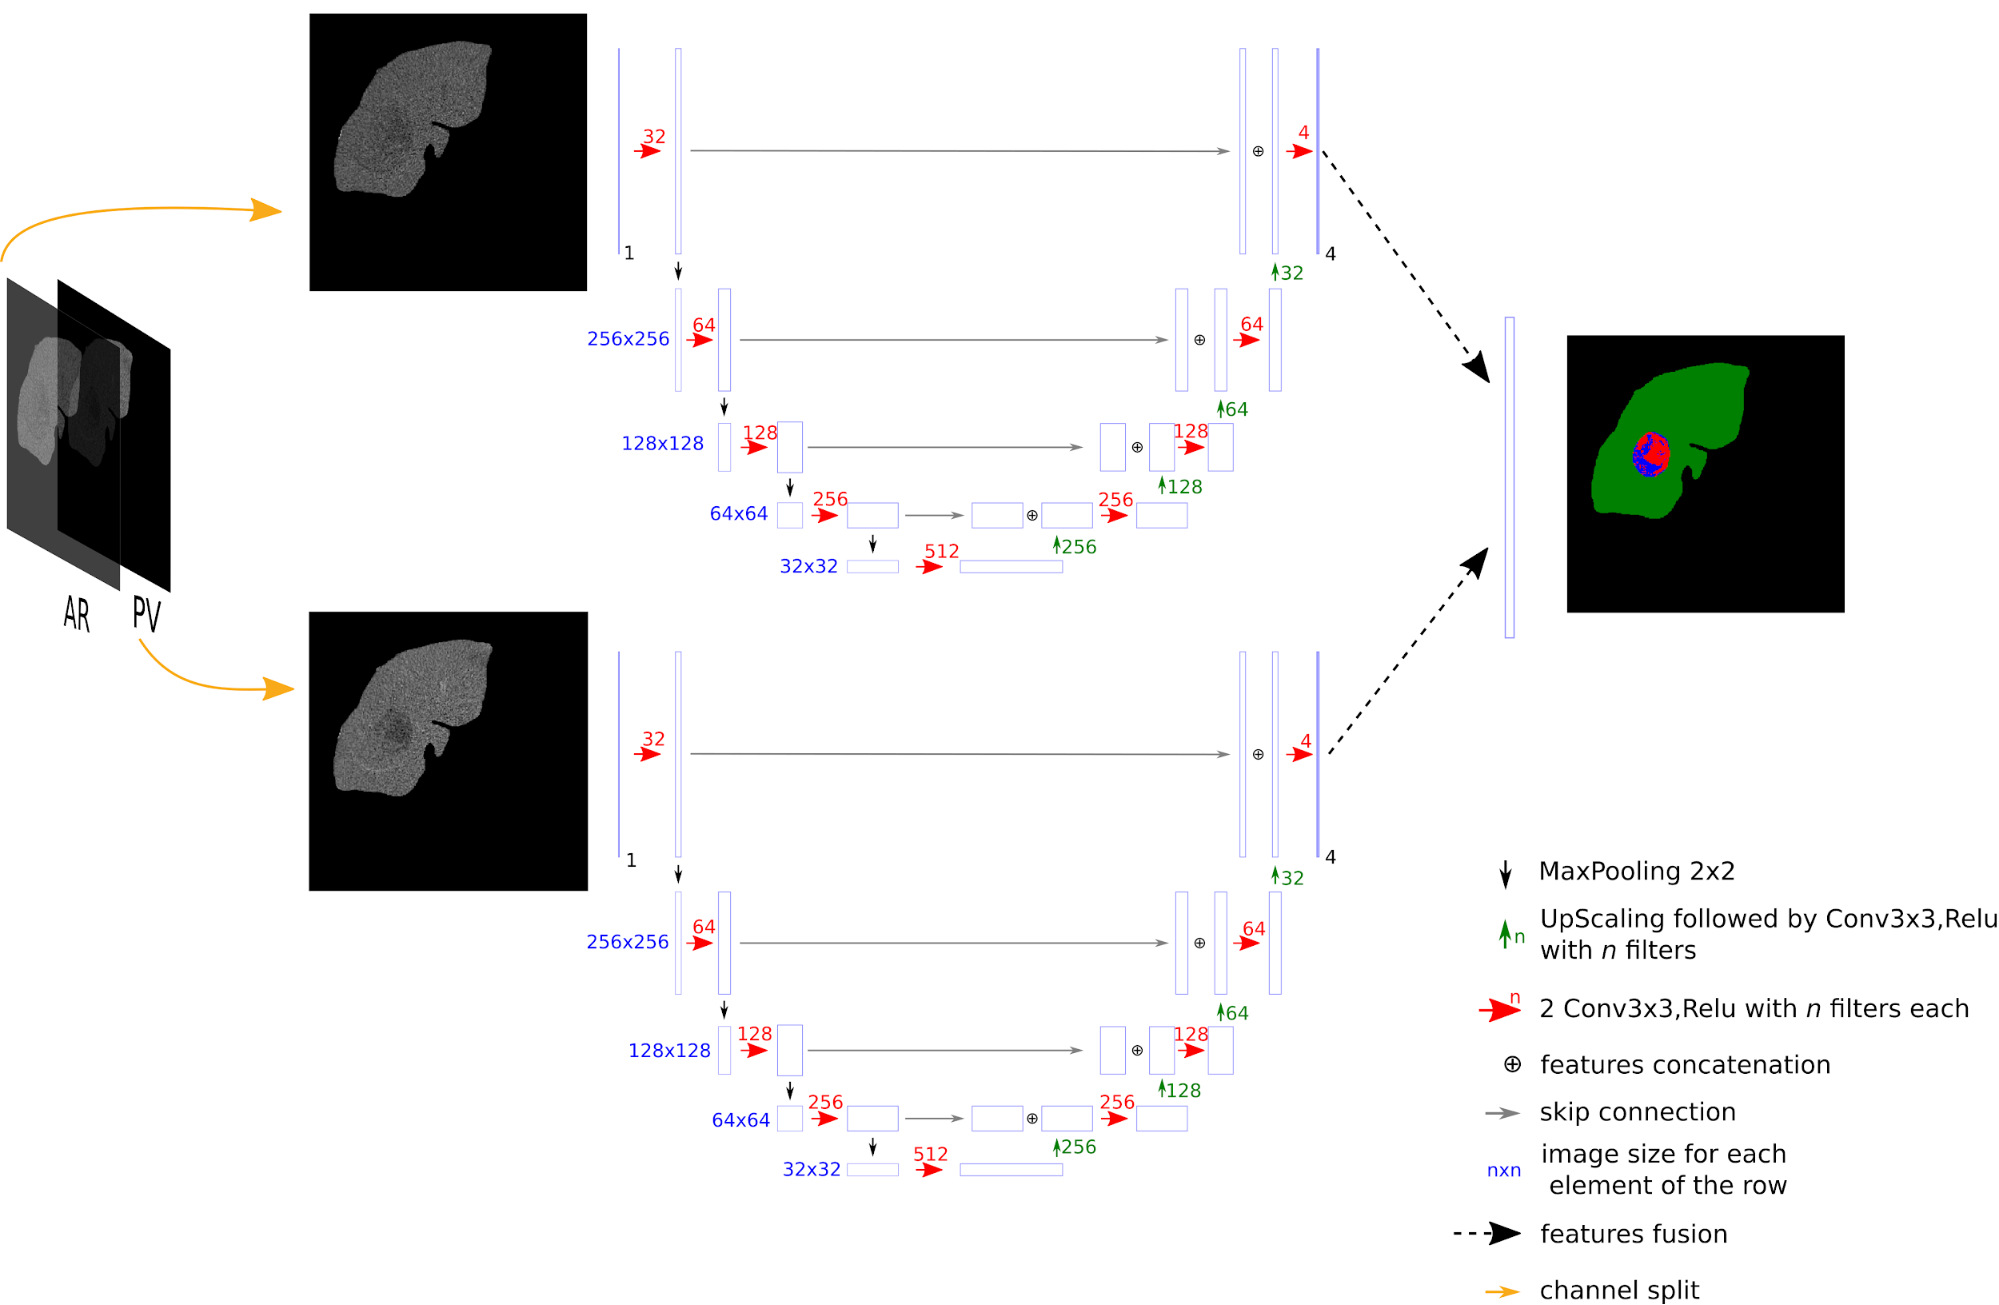
\includegraphics[width=0.9\linewidth]{../SemanticSeg/images/image36}
	\caption{\pplfont{MPF-Full} network: initially, AR and \ac{pv} images are processed separately. The resulting maps are merged (by simple addition) at the end}
	\label{CARS_MPF_Full_Fig}
\end{figure}



\subsection{Datasets}

The different datasets used in our research work are detailed in the
table \ref{xp_datasets}.

\renewcommand{\arraystretch}{2}
\setlength{\tabcolsep}{7pt}
\newgeometry{top=5mm, left=5mm, right=5mm, bottom=10mm, footskip=5mm, headsep=10mm}

\begin{landscape}
\scriptsize
	\begin{longtable}{l|p{2cm}p{1.5cm}p{1.6cm}p{3cm}p{1.5cm}p{1cm}p{1cm}p{1cm}p{1cm}p{1cm}p{1cm}}\toprule
		\textbf{Db Name} & \textbf{Db retained number of cases} & \textbf{Axial voxel size (mm)} & \textbf{Slice Thickness (mm)} & \textbf{Available contrast-enhanced phases} & \textbf{Contains Tumor} & \textbf{Tumor type} & \textbf{Liver  Ground truth} & \textbf{Tumor Ground truth} & \textbf{Necrosis Ground truth}& \textbf{\#Experts} \\
		\midrule
		\textbf{\lmttfont{TheraHCC-dB}} &104 2D slices &0.66-0.97 &0.7-1.25 &NECT, AR \& PV&Yes &HCC & true & true & true &4 \\
		\textbf{\lmttfont{LITS-dB}}& 131  3D vol. & 0.55-1 &0.45-6 &Single phase images but mixed (AR \& PV)&Yes &Mixed & true & true & false &3 \\
		\textbf{\lmttfont{3DIrcad-dB}}\footnote{Subset of the 3DIrcad-01 presented in the table \ref{publicly_available_datasets} where only the 15 volumes with liver tumors were retained} & 15 3D vol. &0.57-0.87 &1.25-4 &Single phase images but mixed (AR \& PV) &Yes &Mixed & true & true & false &- \\
		\textbf{\lmttfont{TCIA-dB}} \footnote{Subset of the one presented in the table \ref{publicly_available_datasets} where only the 18 exploitable volumes with both AR and PV phases were retained} & 18 3D vol. &0.62-0.90 &2.5-7 &AR\&PV&Yes&HCC & false & true & true &1 \\
		\textbf{\lmttfont{G-dB}} & 79  3D vol. &0.58-0.98 &0.8-5 &AR\&PV&Yes &HCC & false & true & false &1 \\
		\bottomrule
		\caption{Datasets used in our experiments (NECT: Non-Enhanced Contrast CT, AR: Arterial, PV: Portal Venous)}\label{xp_datasets}
	\end{longtable}
\end{landscape}

\renewcommand{\arraystretch}{5}
\newgeometry{vmargin={15mm}, hmargin={30mm,30mm}}   % set the margins 

As we can see in the table, and except for \textbf{\lmttfont{LITS-dB}} and \textbf{\lmttfont{3DIrcad-dB}}
(\textbf{\lmttfont{3DIrcad-dB}} being a subset of the \textbf{\lmttfont{LITS-dB}} \cite{Bilic2019}), they are all different in their construction. Differences can
be found on the annotated areas (chosen sparse slices or entire 3D
volumes) and on the annotated tissues that can be found in the dataset
(some of them only contain ground truth annotations for the liver and
the tumors it might contain such as \textbf{\lmttfont{LITS-dB}}, whereas some others contain
only ground truth annotation for the tumor such as \textbf{\lmttfont{TCIA-dB}}). Another
crucial difference concerns the contrast enhanced phases available in
each dataset (\textbf{\lmttfont{LITS-dB}} contains only single phase images whereas \textbf{\lmttfont{TCIA-dB}},
\textbf{\lmttfont{TheraHCC-dB}} and \textbf{\lmttfont{G-dB}} present multiphasic images). \\
To prove the ability of the deep learning to perform the automatic
segmentation of both the liver and its internal tissues, such as the
parenchyma and both the active and the necrotic part of the tumor, we
first performed our experiments on \textbf{\lmttfont{TheraHCC-dB}} since this database was
previously used for the same task \cite{Conze2017}, because it
presents multiphase images and finally because this is the only
available dataset with complete ground truth for both liver parenchyma,
active and necrotic part of the tumors. \\
\textbf{\lmttfont{TheraHCC-dB}} is composed of images from seven patients, all suffering
from \emph{HCC} and who underwent \ac{cect} (Contrast-Enhanced
Computed Tomography) examinations, resulting in a total of 13 \ac{ct}
sequences. \\
More details about the standard \ac{cect} examination protocol can be
found in the chapter \ref{ct-and-mr-imaging}. In our case, images were acquired at 4 different
moments: one before the injection of the contrast medium (\ac{nect}:
Non Enhanced \ac{ct}) , and the 2 others after the injection to reflect both
the arterial (\ac{ar}) (\textasciitilde{}20-25s after injection) and
the portal venous (\ac{pv}) phases (\textasciitilde{}60-70s after
injection).\\
Eight regularly sampled slices across each one the 13 sequences were
segmented by 4 experts, resulting in 104 labeled slices. \\
The segmentation maps obtained from each one the 4 experts were fused
using the STAPLE algorithm to reach a consensus map \cite{Warfield2004}.


\subsection{Experiments}

\subsubsection{Data pre-processing}

The first task to implement in this study was the inter-phase
registration so that environmental effects, such as respiratory motions,
will not affect the performances of the networks, and to ensure that a
given voxel is at the exact same position for the different \ac{cect}
volumes of a patient. The registration was performed using a
diffeomorphic deformable registration algorithm, where the \ac{pv}
images were used as reference, since they contained the original expert
annotations \cite{Avants2008, Conze2017, Ben-Cohen, Christ2017}. \\
Another bias that can affect the deep semantic segmentation networks
training is the heterogeneous image sizes and voxel resolutions present
within the training images.
To avoid this bias, it has been decided to scale them so that they all
have a $ 512\times512 $ axial size \footnote{Either cropping or padding was performed so that the images have the same size} and an isotropic voxel resolution of $ 0.97 \text{mm}^2 $. \\
The data normalization is another aspect that needs to be considered
before feeding the images in the deep network. In order to reduce the
effect of extreme values from regions present in the tomographic images
(such as the bones or the air), and to enhance the intensity of the
liver voxels, we first clipped the \emph{HU} values to be in the range
$ \left[-100, 400\right] $ , corresponding to the most commonly 
observed liver intensities range. The retained intensities were finally mapped to
the interval $ \left[0, 1\right]$ \footnote{\ac{dl} studies usually tend to perform 
data standardization but here HU values are already normalized. 
The used range helps us to avoid potential bias caused by images acquired at a delayed phase with a different contrast}.

\subsubsection{Training}

In order to validate our hypotheses, we have decided to first run
experiments on the \lmttfont{3DIrcad-dB} to set the most crucial hyperparameters
such as the learning rate, the decay, the depth of the network or the
type and the amount of data augmentation.
The selection process is detailed in the chapter \ref{appendix---hyperparameters-selection}, and here is the list of the chosen hyperparameters:

\begin{itemize}
	\item Lr: 1e-4
	\item Decay: 1e-4
	\item Number of epochs: 20
	\item Optimizer: Adam
	\item Number of filters at bottleneck: 1024
	\item Input image size: 512
	\item Data augmentation
	\begin{itemize}
		\item Rotations in the interval $ \left[0, 40\right] $
		\item Translations with shift in the interval $ \left[-0.1, 0.1\right] $
		\item Horizontal and vertical flips
	\end{itemize}
	\item Augmentation factor: 20
\end{itemize}

When transferring those settings to the \textbf{\lmttfont{TheraHCC-dB}}, 
we implemented both translation and the addition of gaussian
noise in the training since it slightly improved the performances.
In order to remove any bias, the same set of hyperparameters has been
used for both the \pplfont{\{.\}-Liver}, \pplfont{\{.\}-Lesion}, \pplfont{\{.\}-Necrosis} and
\pplfont{\{.\}-Full} networks when training the \textbf{\lmttfont{TheraHCC-dB}}, regardless of the
type of input (single phase or multiphase). \\
The same set of hyperparameters was used to train both liver and lesions segmentation networks on repectively the \textbf{\lmttfont{LITS-dB}} and the \textbf{\lmttfont{G-dB}}.

We first present the results obtain when performing the semantic segmentation of liver tissues on the \textbf{\lmttfont{TheraHCC-dB}}, before applied the resulting architecture to provide additional annotations to both \textbf{\lmttfont{TCIA-dB}} and \textbf{\lmttfont{G-dB}}.


\subsubsection{Semantic segmentation of liver tissues}

In this section, mean \ac{dsc}s were computed in a slice-wise fashion for each target class and the different methods were statistically compared using the Wilcoxon 
signed paired rank tests, since slice-wise \ac{dsc}s did not follow a normal distribution. 
We first compared \pplfont{\{\ac{nect}, \ac{ar}, \ac{pv}, DMP, MPF\}-Liver} networks
 to evaluate which phase allows better liver segmentation. 
 We then trained \pplfont{\{\ac{nect}, \ac{ar}, \ac{pv}, DMP, MCF\}-Lesion} and  \pplfont{\{\ac{nect}, \ac{ar}, \ac{pv}, DMP, MCF\}-Necrosis} networks separately on the \textbf{\lmttfont{TheraHCC-dB}} by masking all values outside the liver using ground truth annotations in order to assess whether multiphase information is really useful for the segmentation. The results are given in table \ref{SingleVsMult}.

Multiphase performed significantly better than single-phase for segmenting the liver (DMP vs \ac{pv}, $P=0.001$; DMP vs \ac{ar}, $P=0.005$, DMP vs \ac{nect}, $P<0.001$) and the active part of the lesions (DMP vs \ac{pv}, $P<0.001$; DMP vs \ac{ar}, $P=0.003$; DMP vs \ac{nect}, $P<0.001$). When comparing single-phase alone, \ac{pv} achieved significantly better \ac{dsc}s than \ac{ar} or \ac{nect} for all the segmentation tasks except for the liver segmentation. When comparing multiphase methods, DMP carries out significantly better than MPF for the segmentation of the liver (DMP vs MPF, $P=0.004$), the parenchyma (DMP vs MPF, $P<0.001$) and the active part of the lesions (DMP vs MPF, $P=0.005$).

Since both \pplfont{DMP-Lesion} and \pplfont{DMP-Necrosis} led to the best results, we combined them in a cascade as explained before, and compared it to both \pplfont{\{\ac{nect}, \ac{ar}, \ac{pv}, DMP, MPF\}-Full} networks. We evaluated them in terms of liver tissue classification performance on images where the values outside the ground truth liver area were masked. The mean \ac{dsc}s are reported in table \ref{FullvsCascade}. Examples of segmentation results are given in figure \ref{CompareFullCascade}. \\

\renewcommand{\arraystretch}{1}
\begin{table}[ht!]
\caption{Segmentation results using single-phase vs multiphase methods on \lmttfont{TheraHCC-dB}.}
\begin{tabular}{llccccc}
\cline{1-7}
\multicolumn{1}{l}{Input}& \multicolumn{1}{l}{Target} & \multicolumn{5}{l}{Network} \\
\cline{3-7}
\multicolumn{1}{c}{}& \multicolumn{1}{c}{} & \multicolumn{1}{c}{\pplfont{\ac{nect}}} & \multicolumn{1}{c}{\pplfont{\ac{ar}}} & \multicolumn{1}{c}{\pplfont{\ac{pv}}} & \multicolumn{1}{c}{\pplfont{DMP}} & \multicolumn{1}{c}{\pplfont{MPF}} \\
\cline{1-7}
Raw \ac{ct} & Liver & 81.1 $\pm$ 27.7 & 89.5 $\pm$ 13.2 & 88.7 $\pm$ 11.4 & $\mathbf{89.9 \pm 15.6}$ & 88.2 $\pm$ 16.0 \\
True liver mask & Parenchyma & 86.5 $\pm$ 13.7 & 82.5 $\pm$ 18.6 & 88.7 $\pm$ 15.4 & $\mathbf{90.5 \pm 13.2}$ & 86.9 $\pm$ 17.8 \\
True liver mask & Lesion & 77.4 $\pm$ 24.1 & 77.4 $\pm$ 20.2 & 87.8 $\pm$ 9.7 & $\mathbf{88.5 \pm 11.7}$ & 86.6 $\pm$ 10.3 \\

True lesion mask & Necrosis & 67.5 $\pm$ 15.5 & 69.7 $\pm$ 16.3  & 77.8 $\pm$ 12.4 & 78.5 $\pm$ 13.3 & $\mathbf{78.8 \pm 11.7}$ \\
True lesion mask & Active Tumor & 65.6 $\pm$ 20.4 & 63.9 $\pm$ 22.6 & 71.6 $\pm$ 20.7 & $\mathbf{75.5 \pm 17.4}$ & 73.2 $\pm$ 18.6 \\
\cline{1-7}
\end{tabular}
\label{SingleVsMult}
\end{table}

\begin{table}[ht!]
\caption{Segmentation results using \pplfont{\{$ \cdot$\}-Full} vs cascaded architectures on \lmttfont{TheraHCC-dB}.}
\begin{tabular}{lcccccc}
\cline{1-7}
\multicolumn{1}{l}{Target} & \multicolumn{6}{l}{Network} \\
\cline{2-7}
\multicolumn{1}{c}{}& \multicolumn{1}{c}{\pplfont{\ac{nect}-Full}} & \multicolumn{1}{c}{\pplfont{\ac{ar}-Full}} & \multicolumn{1}{c}{\pplfont{\ac{pv}-Full}} & \multicolumn{1}{c}{\pplfont{DMP-Full}} & \multicolumn{1}{c}{\pplfont{MPF-Full}} &
\multicolumn{1}{c}{Cascaded DMP}\\
\cline{1-7}
Parenchyma & 85.3 $\pm$ 14.9 & 84.1 $\pm$ 17.9 & 87.0 $\pm$ 19.0  & 82.9 $\pm$ 19.7 & 87.9 $\pm$ 15.9 & $\mathbf{90.5 \pm 13.2}$\\
Necrosis & 62.6 $\pm$ 18.6 & 63.5 $\pm$ 21.5 & 75.7 $\pm$ 14.4 & 73.7 $\pm$ 14.1 & 75.6 $\pm$ 13.4 & $\mathbf{75.8 \pm 15.1}$ \\
Active Tumor & 42.2 $\pm$ 24.0 & 43.2 $\pm$ 26.1 & 53.5 $\pm$ 24.2 & 51.3 $\pm$ 25.6 & 52.0 $\pm$ 23.3 & $\mathbf{59.6 \pm 22.5}$ \\
\cline{1-7}
\end{tabular}
\label{FullvsCascade}
\end{table}

The results highlighted that the cascaded version performed significantly better than \pplfont{\{$ \cdot$\}-Full} networks for segmenting the active part of the lesion (Cascaded DMP vs \pplfont{\ac{pv}-Full}, $P = 0.001$).
The resulting segmentation maps allow us to estimate the necrosis rate (which will be the ratio between the necrotic and the tumor areas). This metric is commonly used for diagnosis and prognosis of the treatment outcome. In this configuration\footnote{after using the liver expert \ac{gt} as mask for the first step}, our workflow provided estimates of this valuable biomarker with a mean error rate of 13.0 \%, which is accurate enough for clinical application. \\

When compared with another study that have been using a different dataset composed of MR images, we achieved slightly better segmentation results \cite{Zhang}.
We evaluated our method on the same database used in \cite{Conze2017}, where a manual expert interaction was required for the segmentation phase, which is not the case in the present deep learning approach. To allow fair comparison, the evaluation was conducted on the areas where all the experts reached an agreement as in \cite{Conze2017}. The mean patient-wise segmentation \ac{dsc}s are depicted in table \ref{ComparisionConze}. Our method enabled a better segmentation of the lesions and both necrotic and active parts. Therefore, we were able to predict the patient-wise necrosis rate with a slightly better precision. 

\begin{table}[ht!]
\caption{Average patient-wise segmentation \ac{dsc}s (on full agreement expert area) with the semi-interactive approach of \cite{Conze2017} and the cascaded DMP method}
\begin{tabular}{lcc}
\hline
& Semi-interactive method \cite{Conze2017} & ours \\
\hline
Parenchyma & \textbf{93.7 $\pm$ 3.4} & 92.2 $\pm$ 4.7 \\
Lesion & 90.7 $\pm$ 6 & \textbf{91.8 $\pm$ 4} \\
Necrosis & 83.0 $\pm$ 12.9 & \textbf{83.6 $\pm$ 11.7} \\
Active Tumor & 75.2 $\pm$ 10.9 & \textbf{82.0 $\pm$ 6.4} \\
Necrosis rate error & 7.84 $\pm$ 4.4 & \textbf{7.10 $\pm$ 1.4} \\
\hline
\end{tabular}
\label{ComparisionConze}
\end{table}

\begin{figure}[!ht]
\centering
\begin{minipage}{4cm}
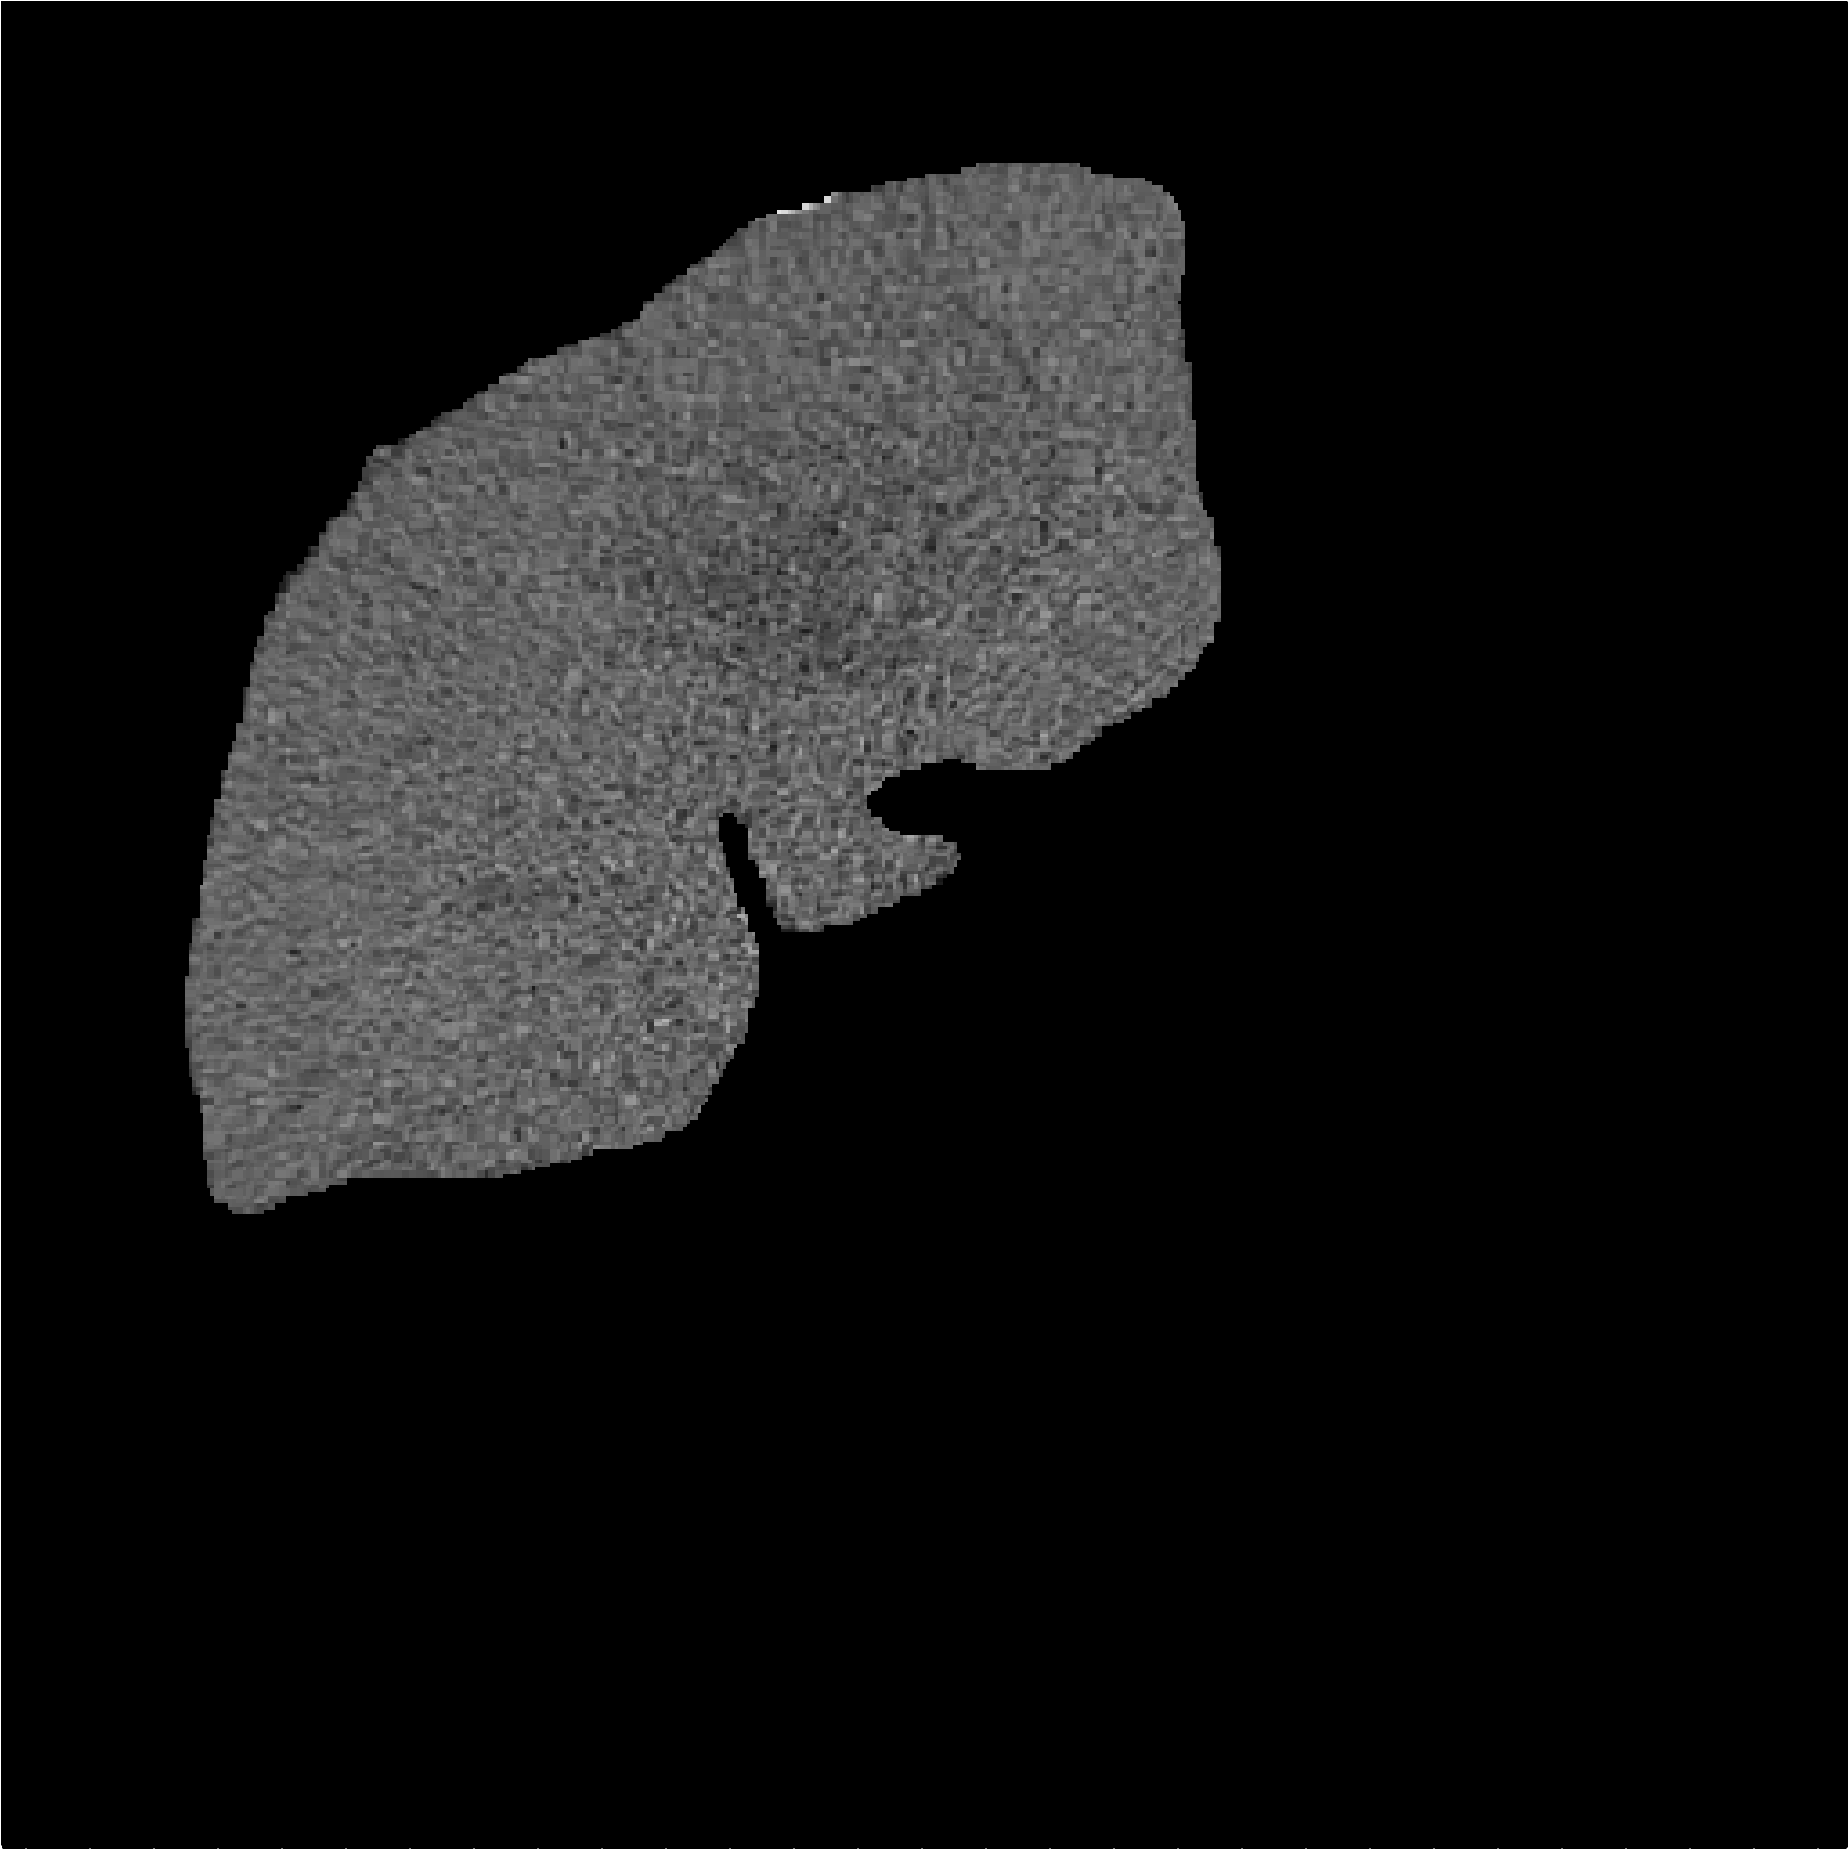
\includegraphics[width=\linewidth]{../SemanticSeg/images/1_21_orig_resized}
\end{minipage} \hspace{-0.3cm}
\begin{minipage}{4cm}
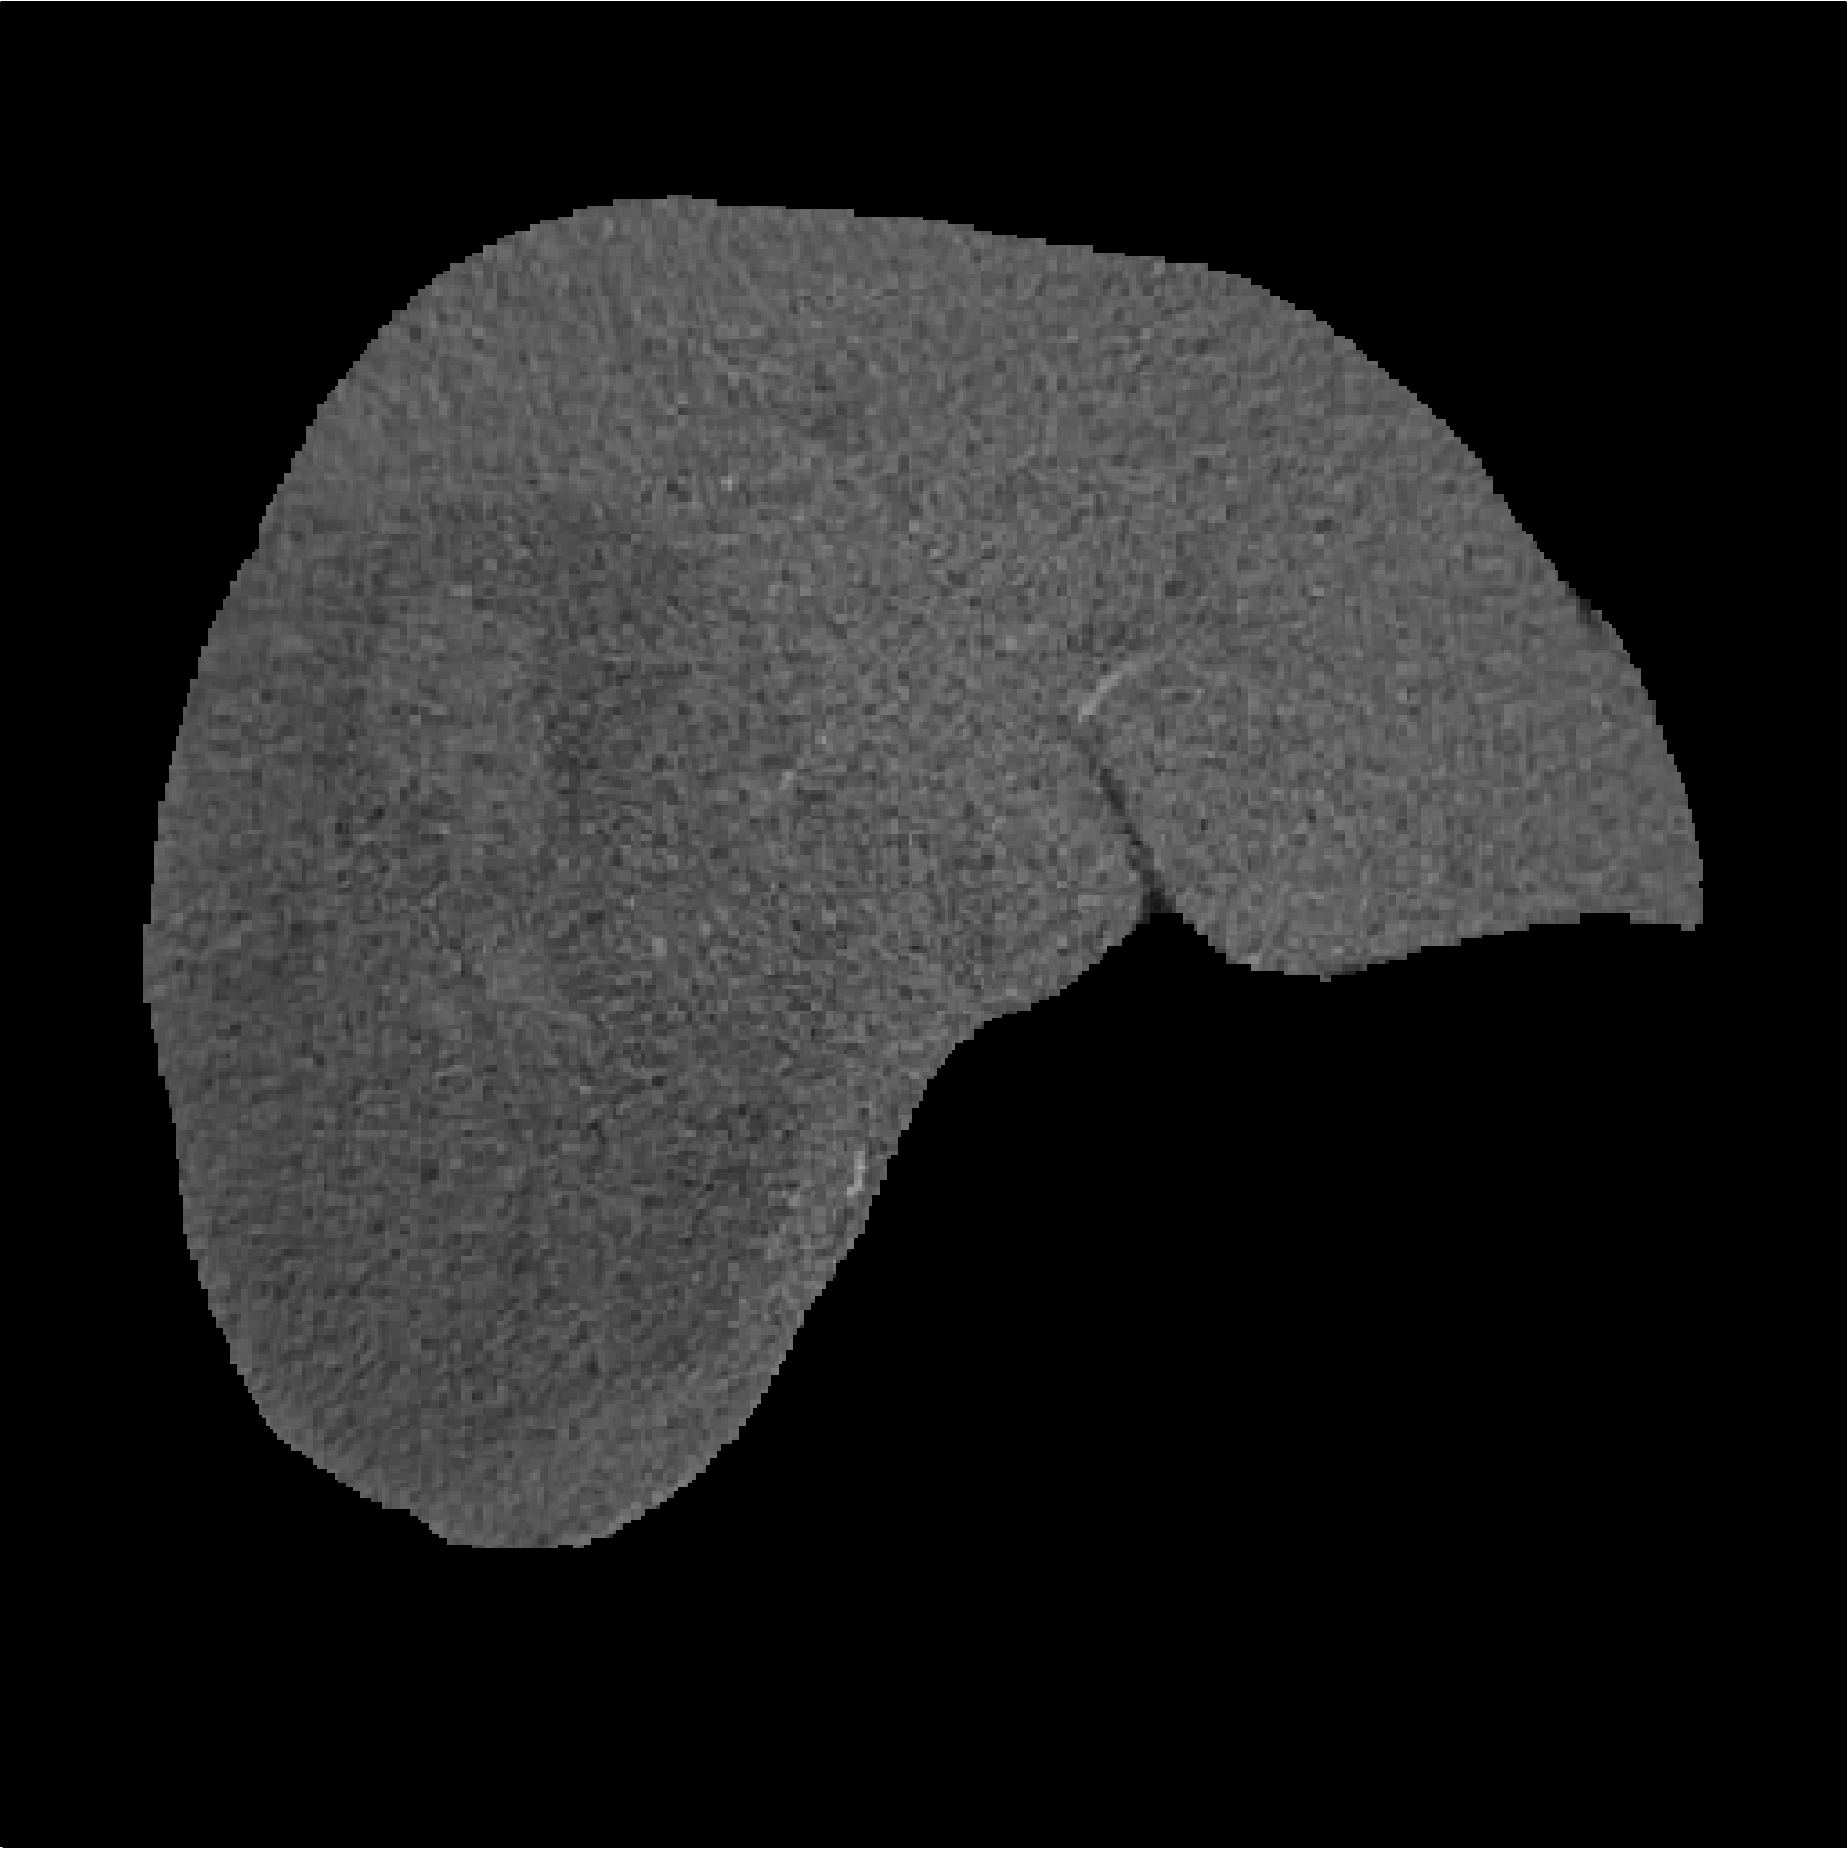
\includegraphics[width=\linewidth]{../SemanticSeg/images/5_2_orig_resized}
\end{minipage} \hspace{-0.3cm}
\begin{minipage}{4cm}
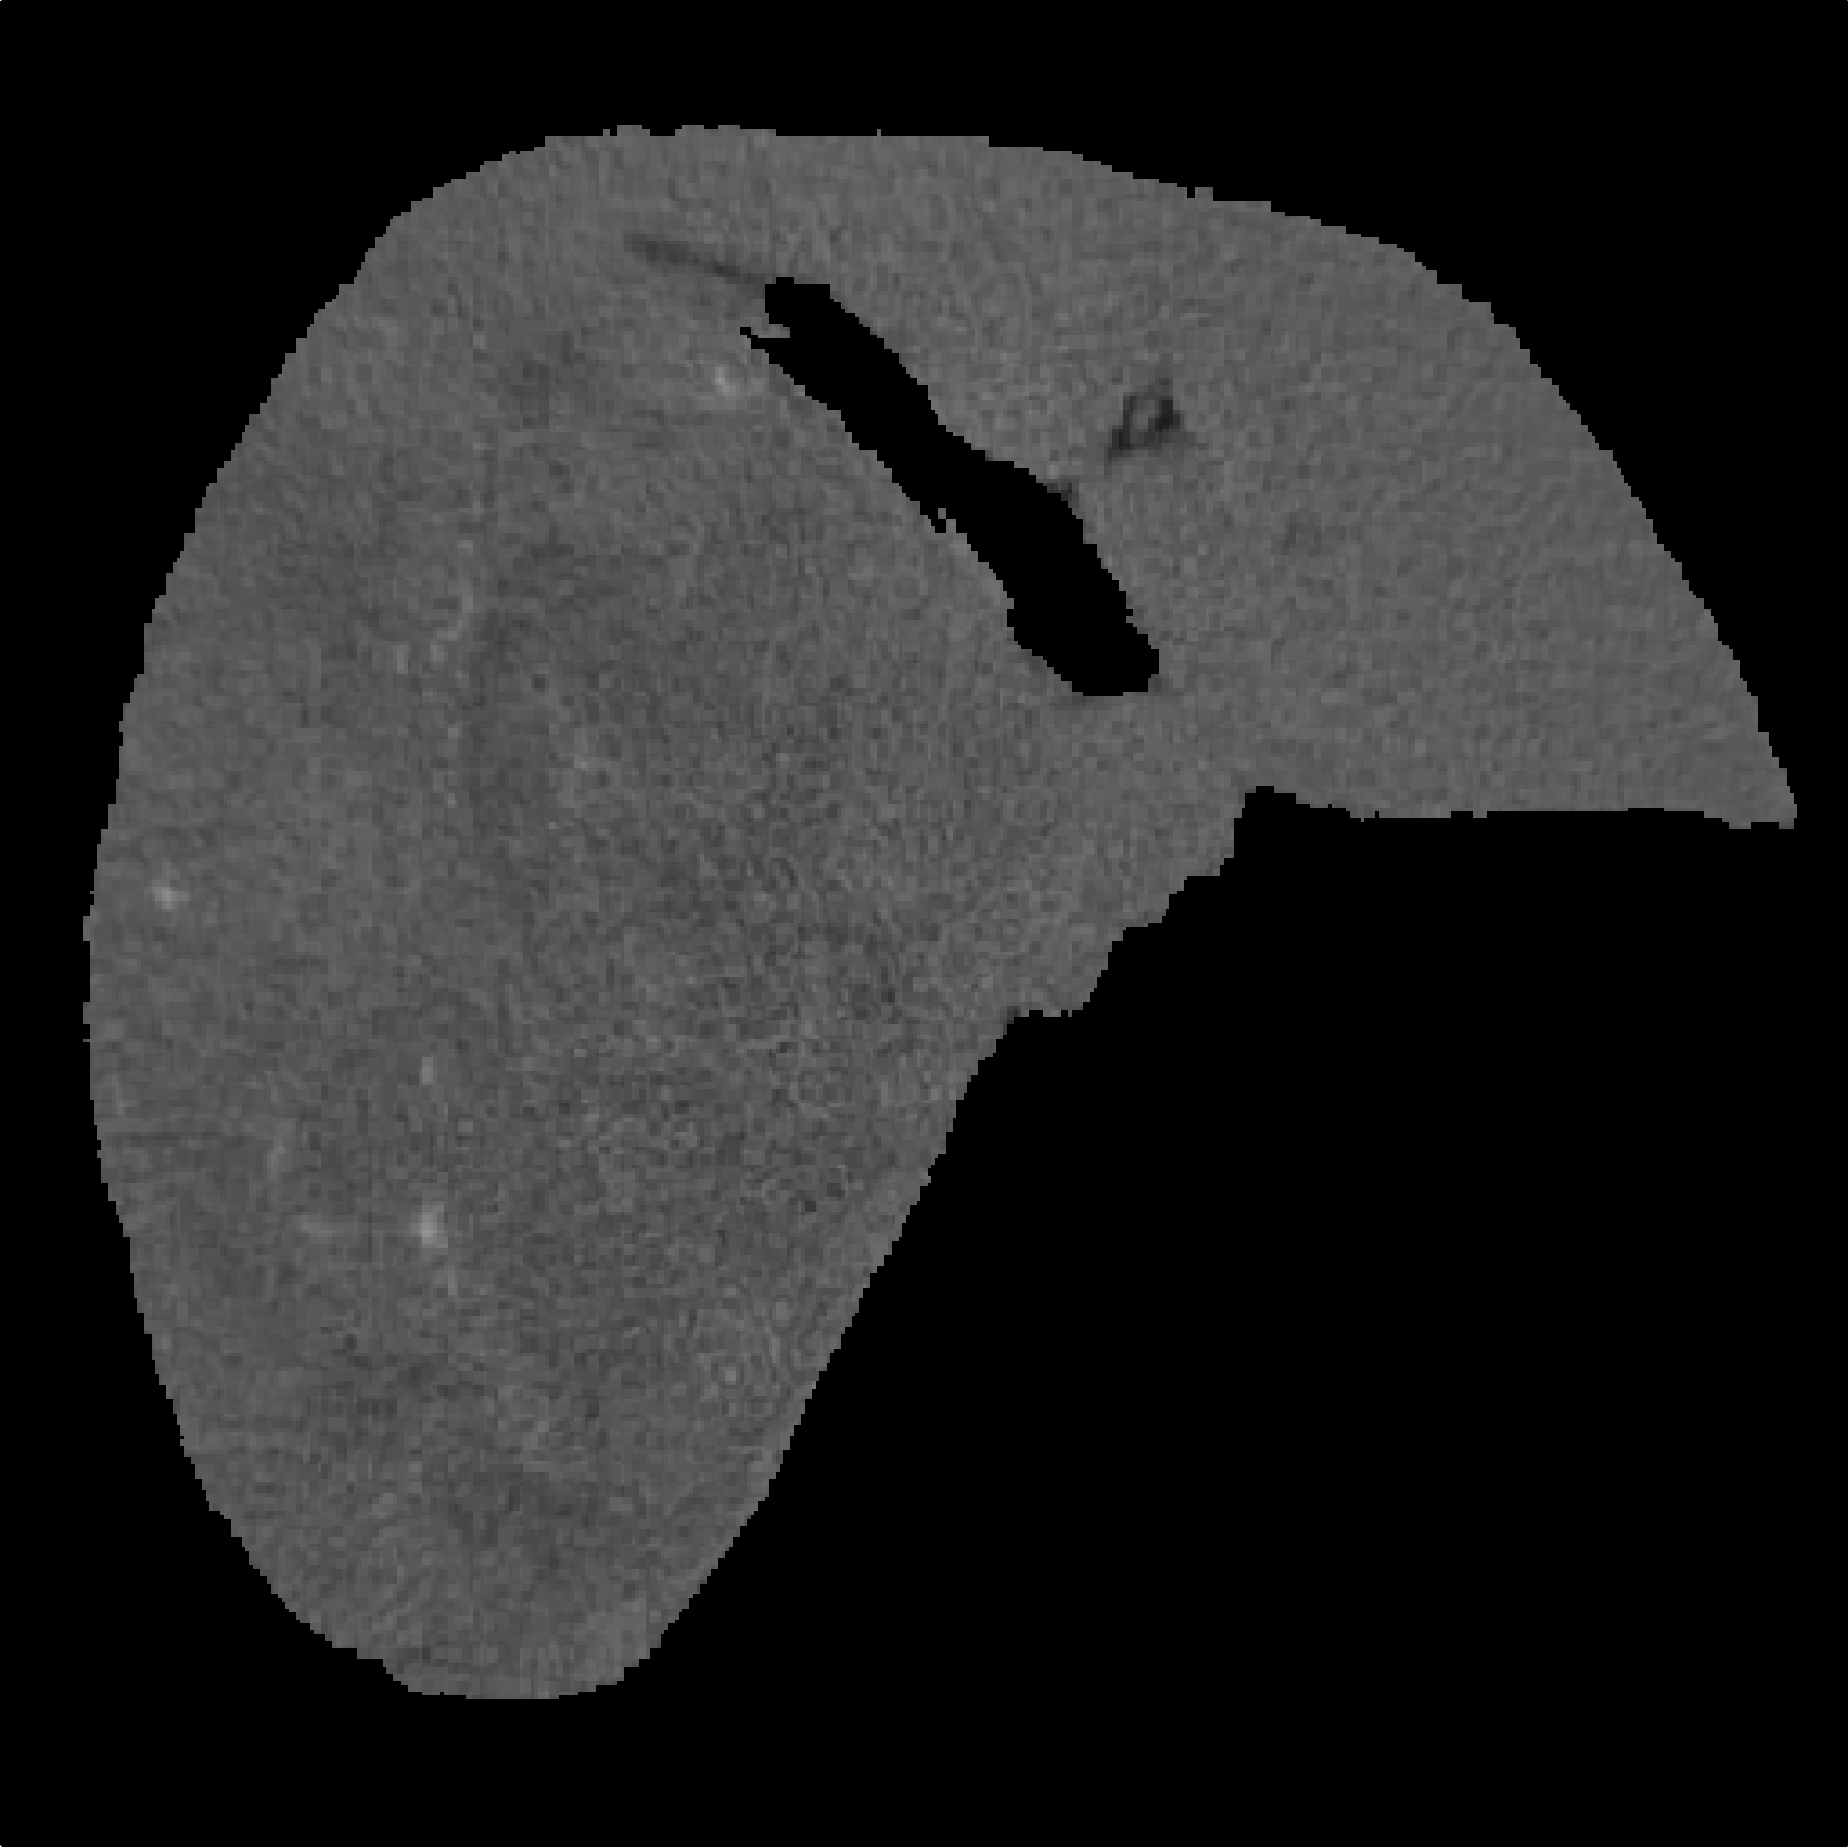
\includegraphics[width=\linewidth]{../SemanticSeg/images/5_8_orig_resized}
\end{minipage}
\vspace{-0.2cm}
\begin{minipage}{4cm}
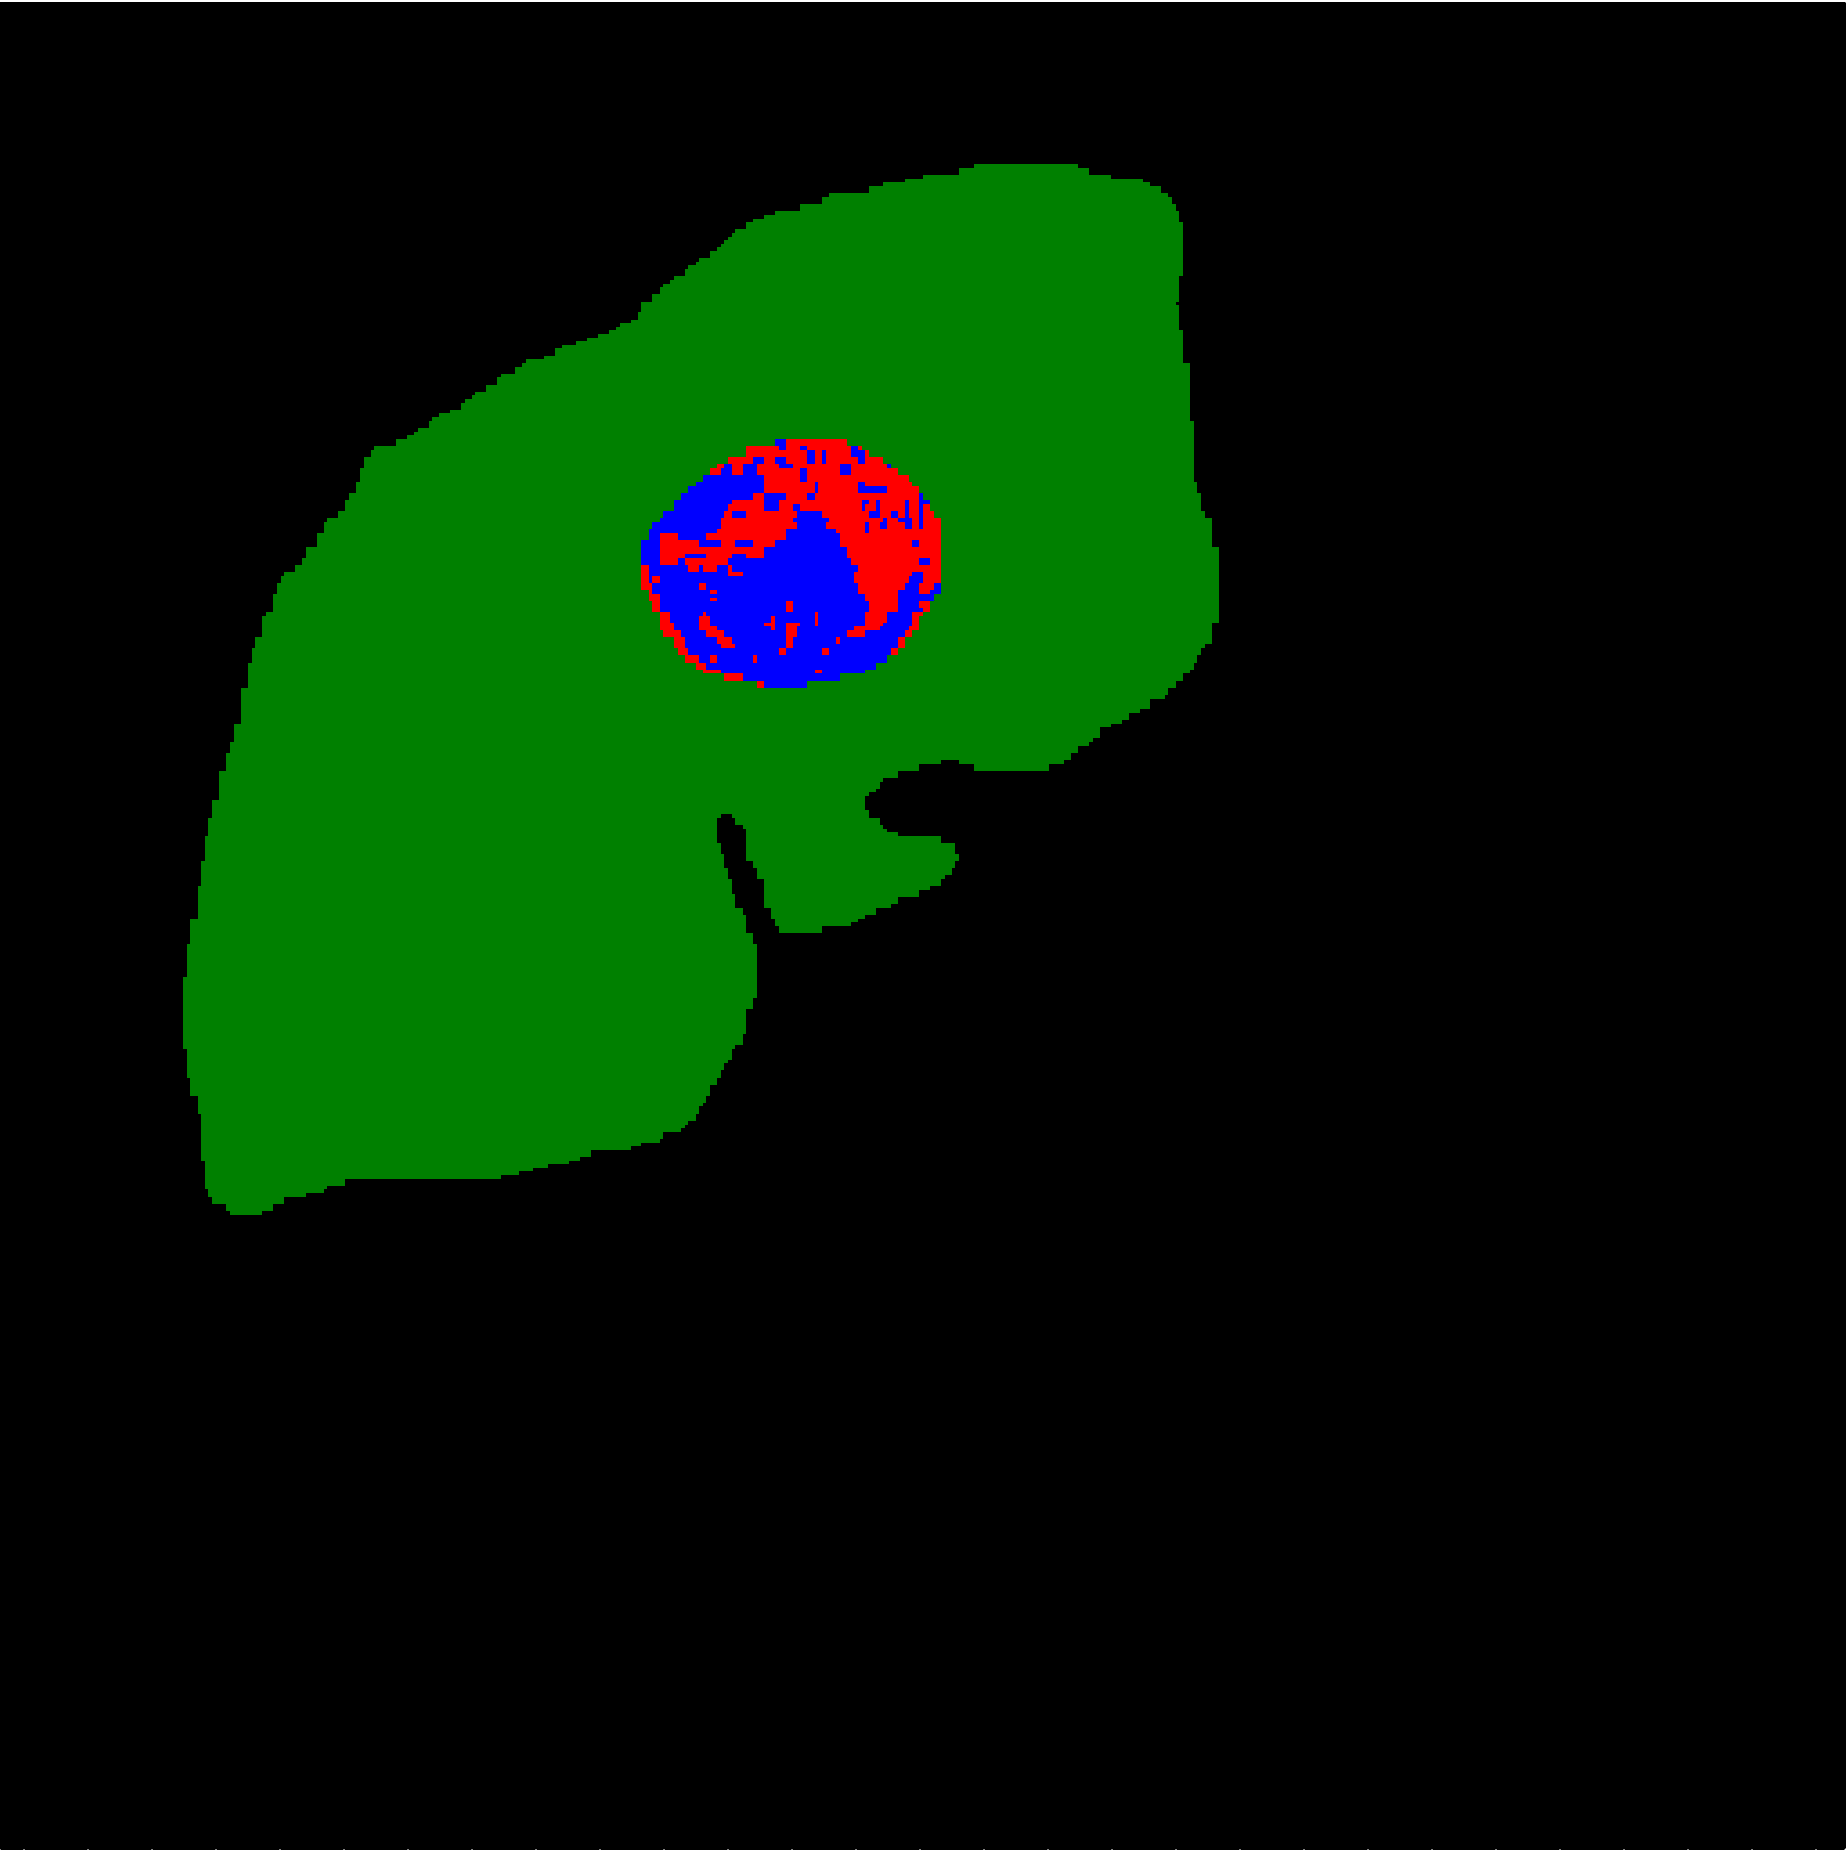
\includegraphics[width=\linewidth]{../SemanticSeg/images/1_21_gt_resized}
\end{minipage} \hspace{-0.3cm}
\begin{minipage}{4cm}
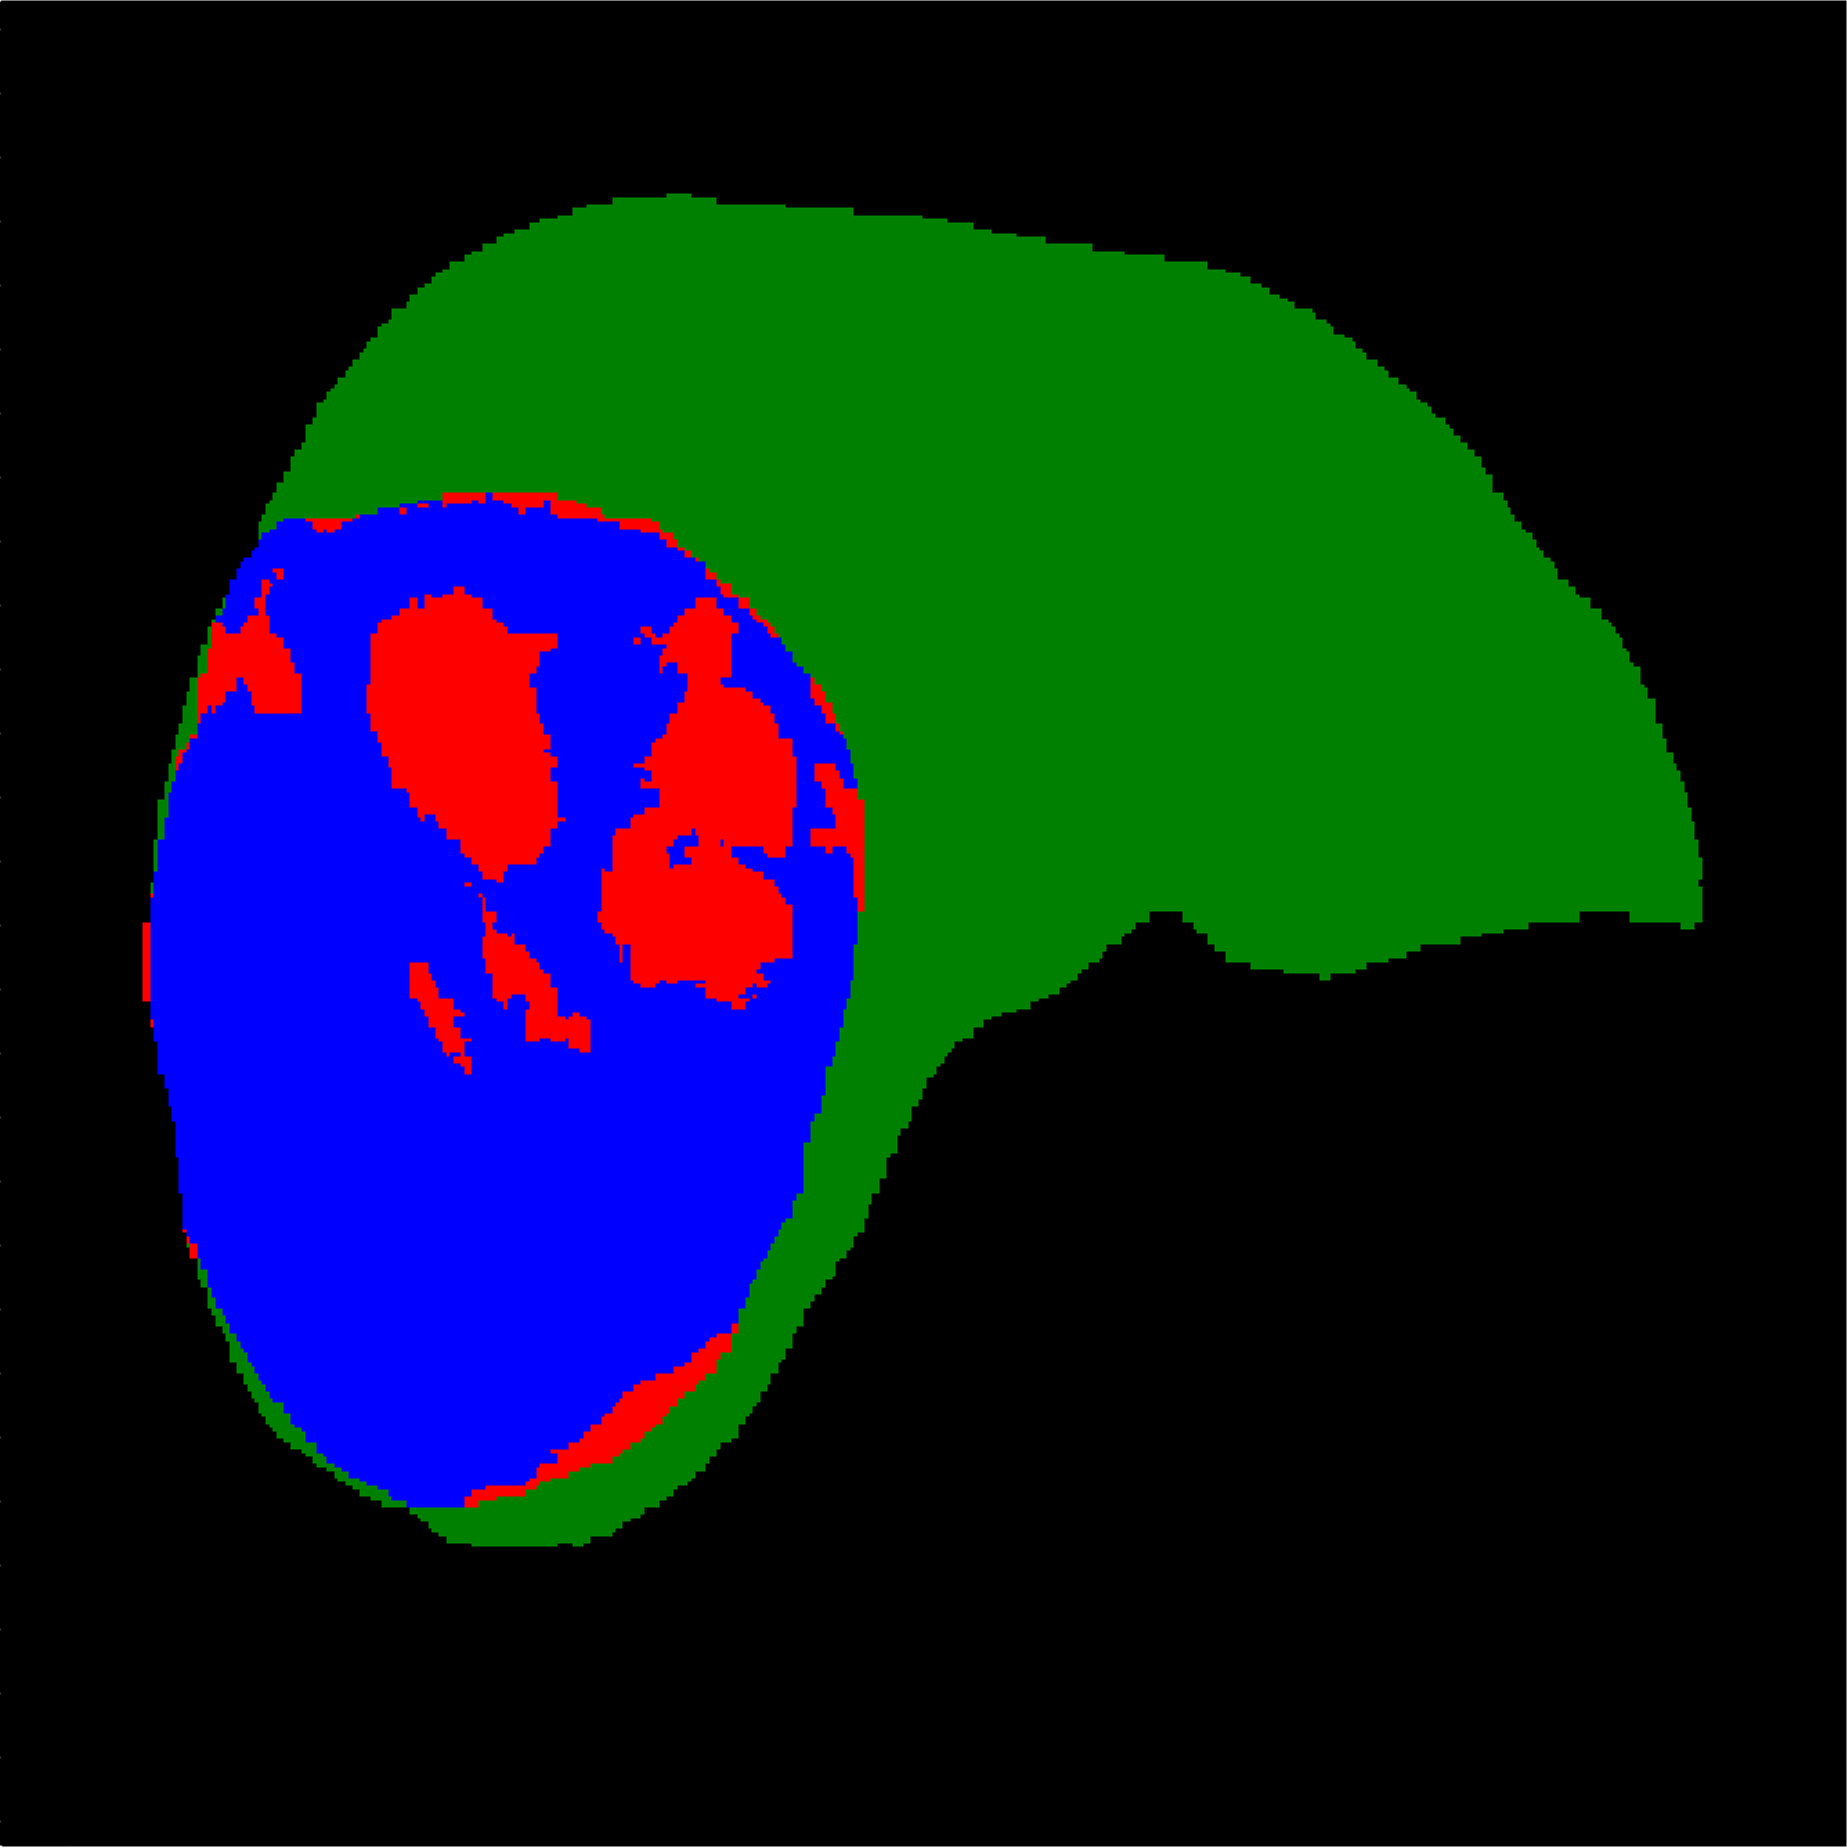
\includegraphics[width=\linewidth]{../SemanticSeg/images/5_2_gt_resized}
\end{minipage} \hspace{-0.3cm}
\begin{minipage}{4cm}
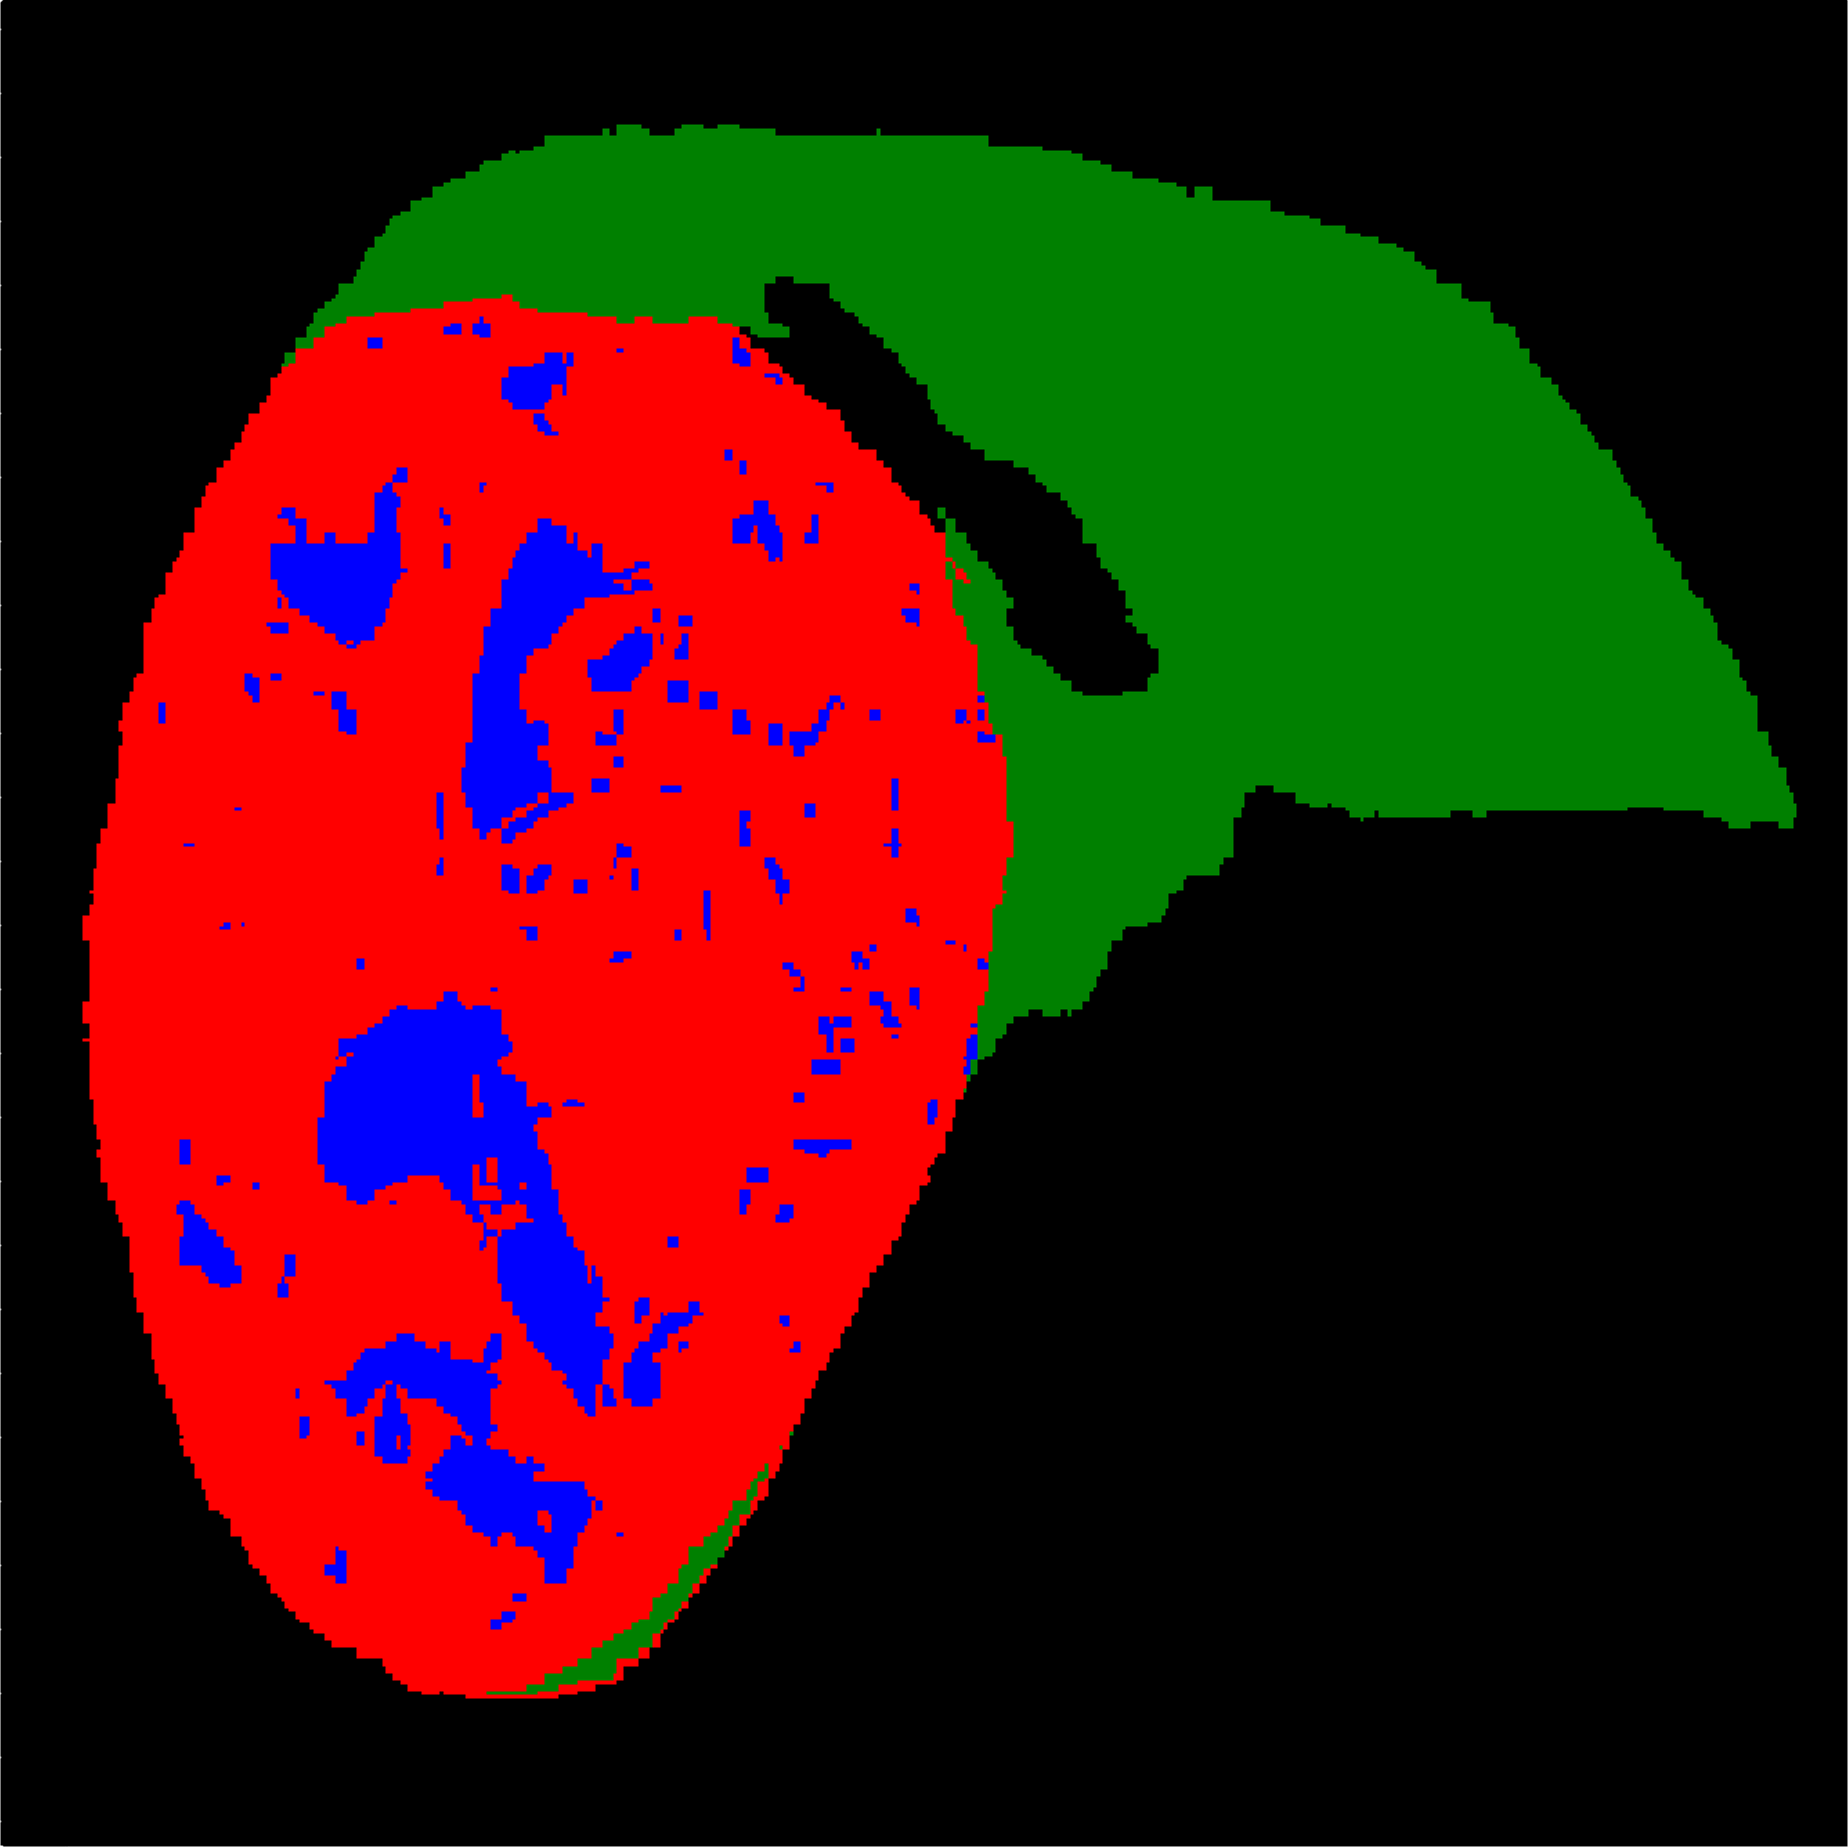
\includegraphics[width=\linewidth]{../SemanticSeg/images/5_8_gt_resized}
\end{minipage} 
\vspace{-0.2cm}
\begin{minipage}{4cm}
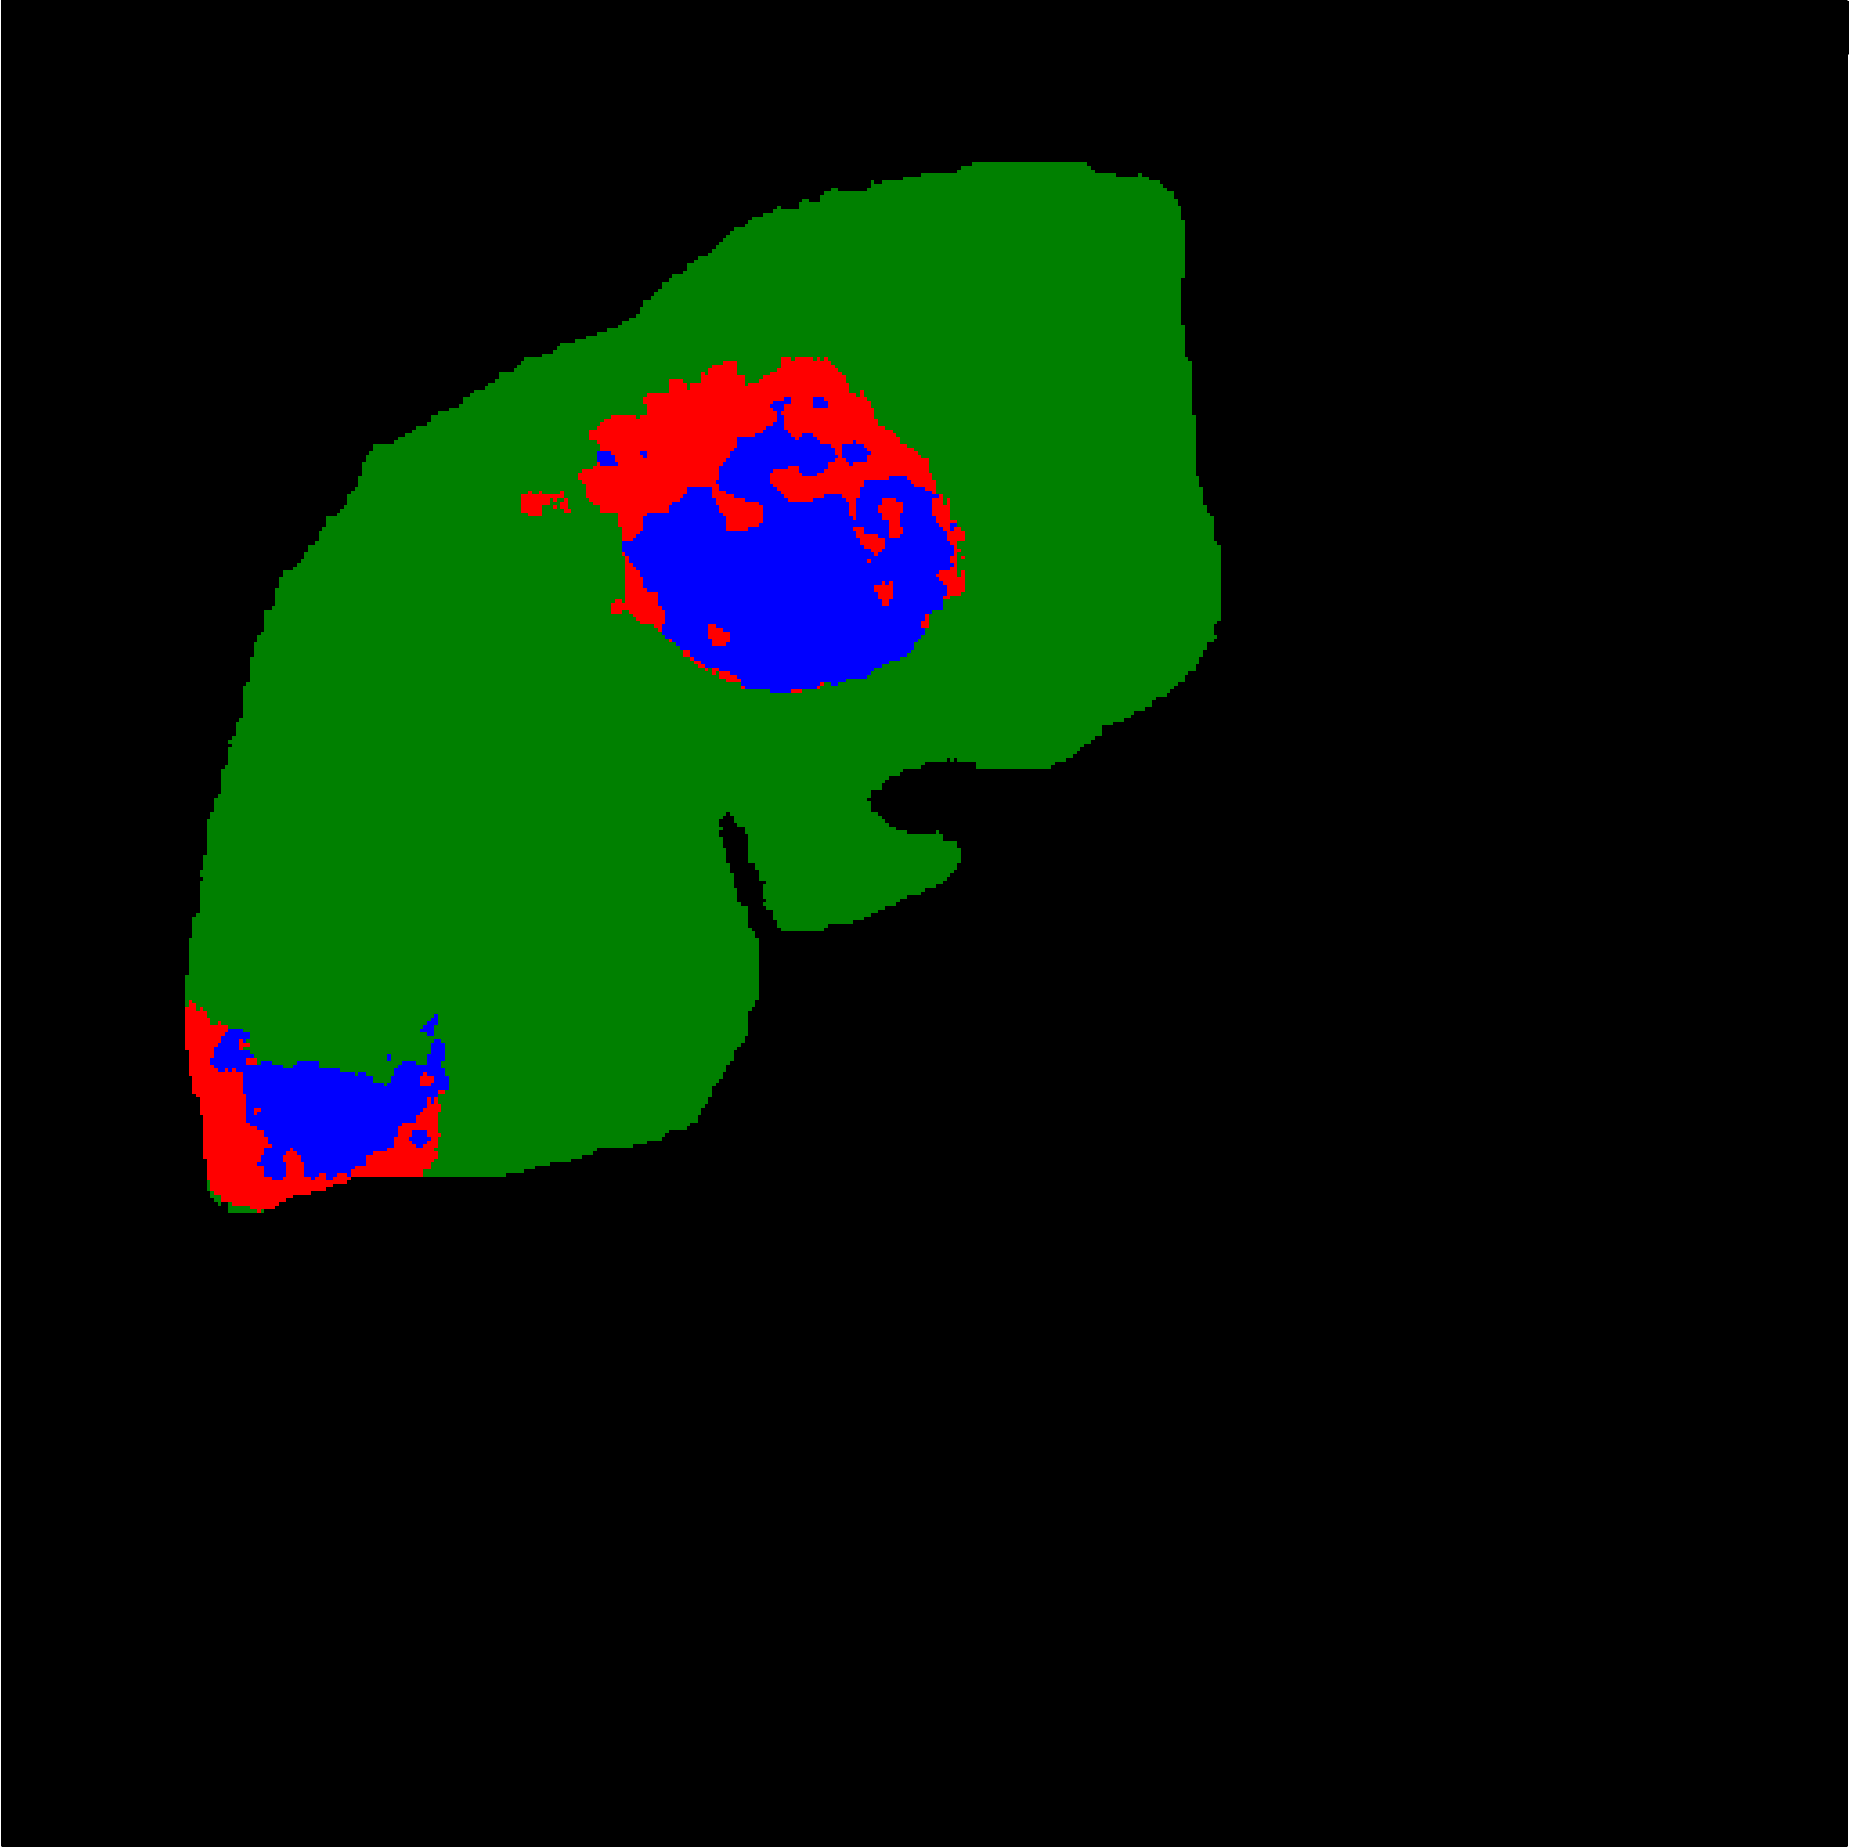
\includegraphics[width=\linewidth]{../SemanticSeg/images/1_21_FullDMP_resized}
\end{minipage} \hspace{-0.3cm}
\begin{minipage}{4cm}
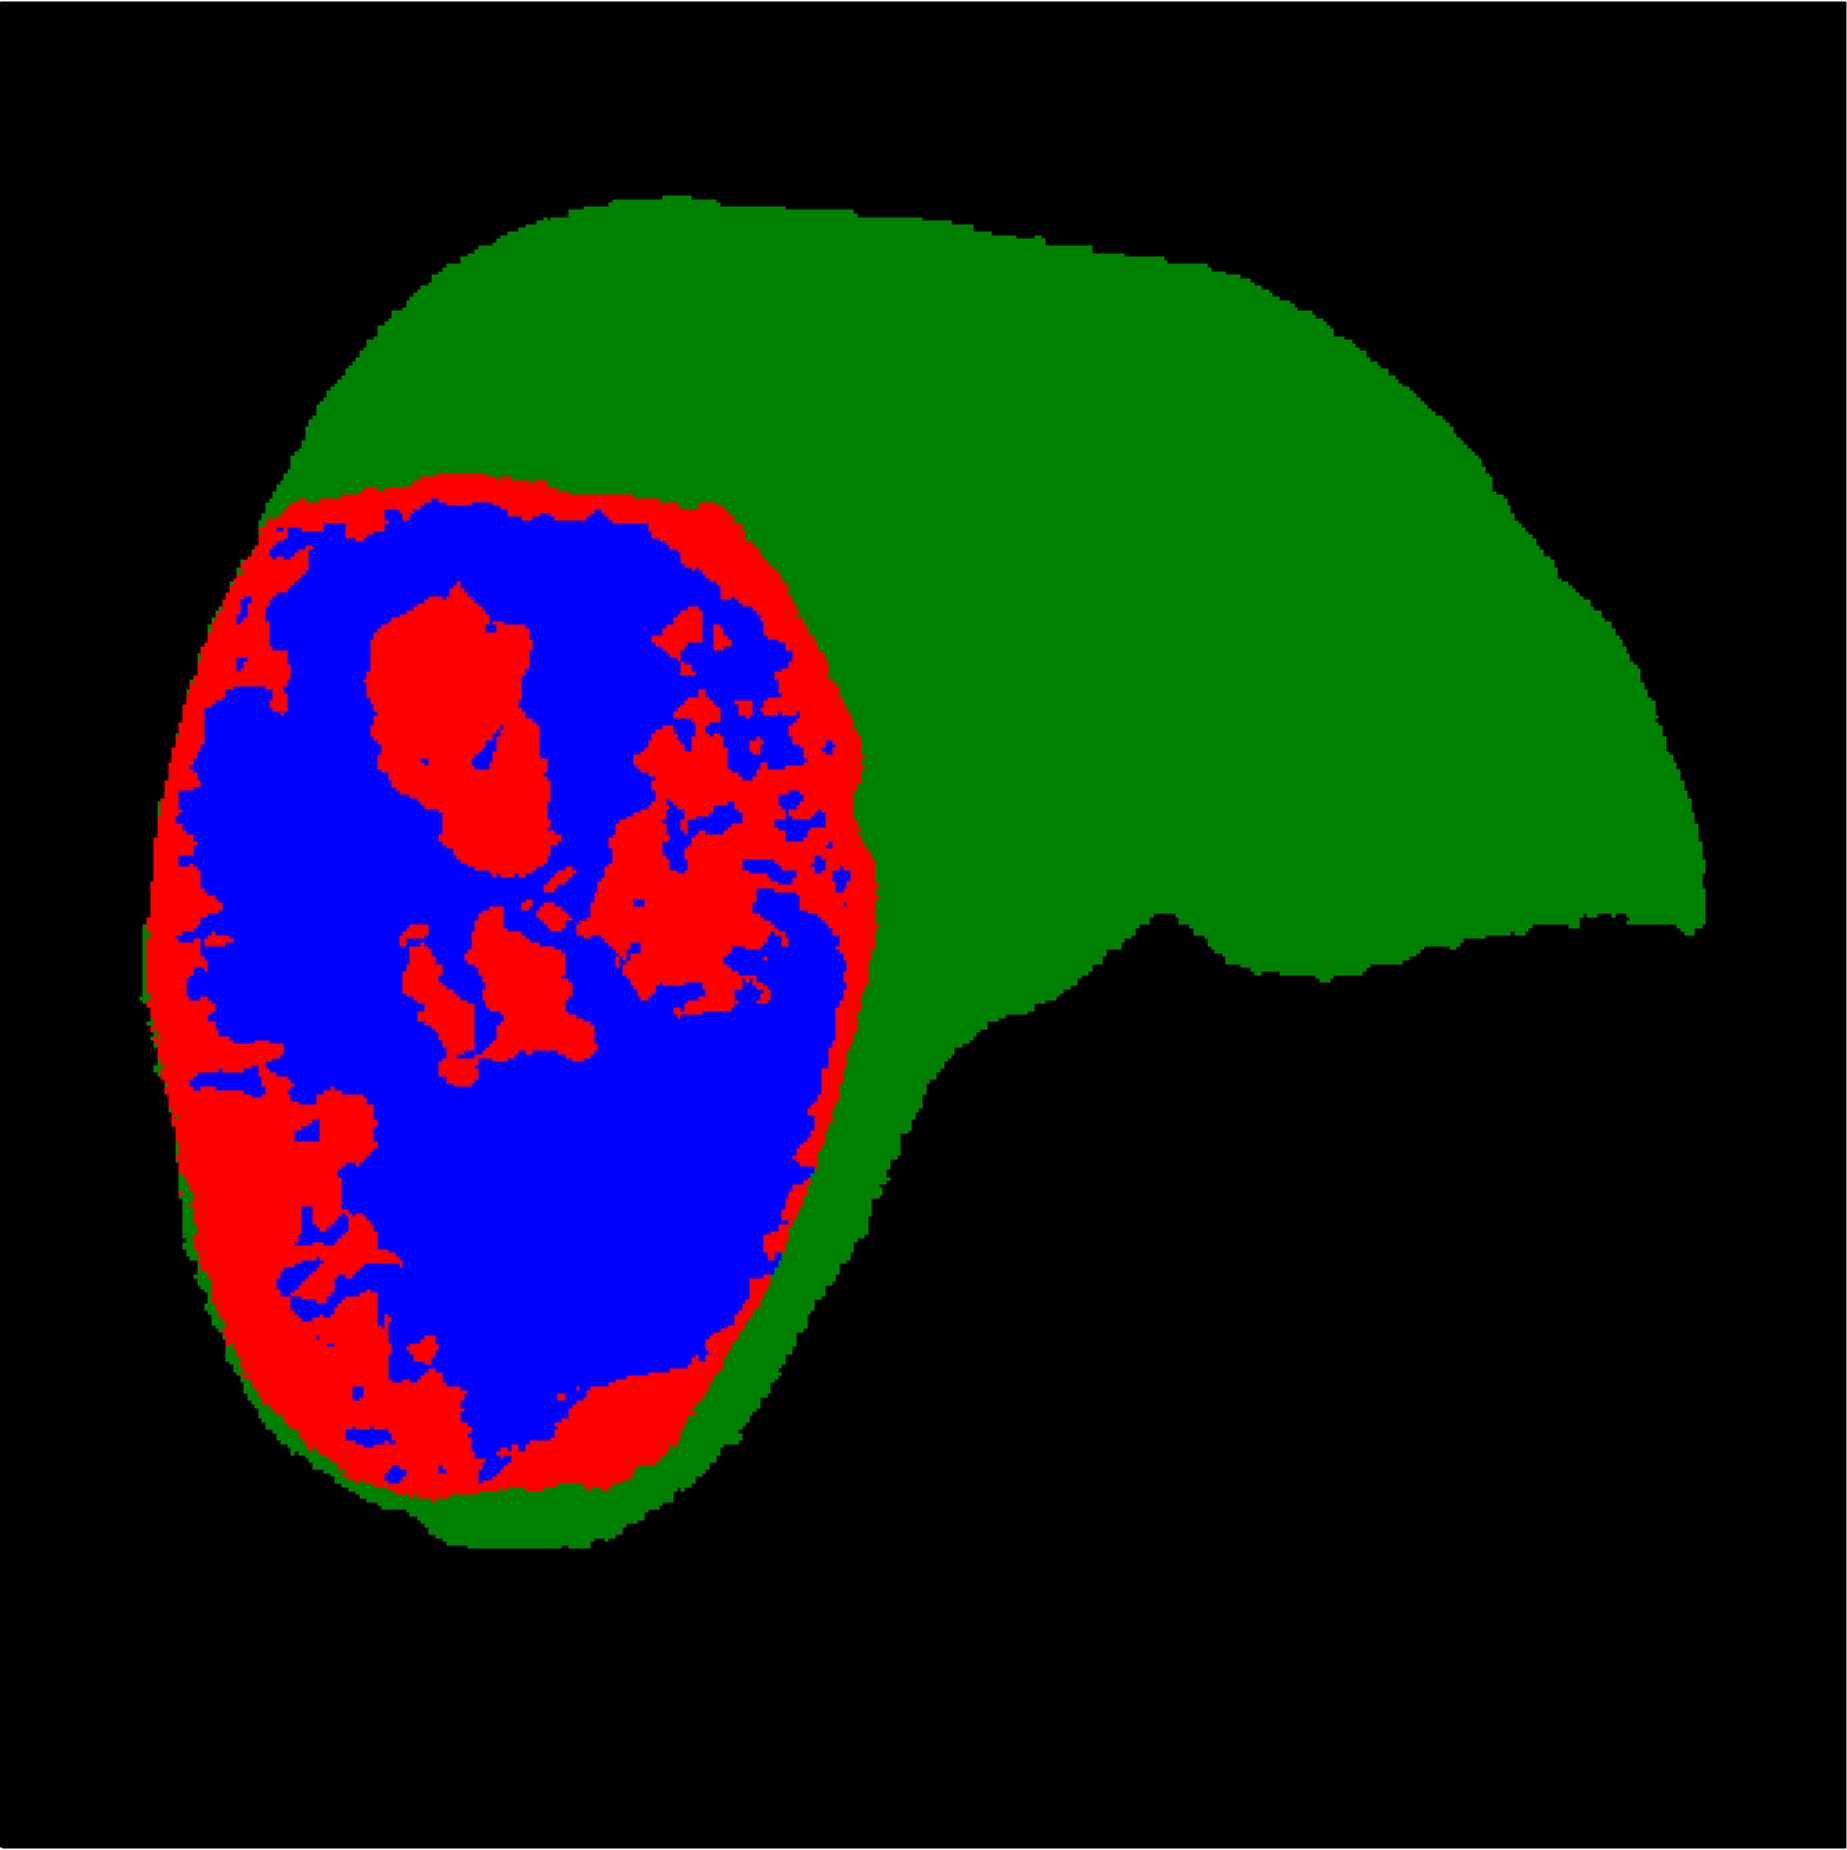
\includegraphics[width=\linewidth]{../SemanticSeg/images/5_2_FullDMP_resized}
\end{minipage} \hspace{-0.3cm}
\begin{minipage}{4cm}
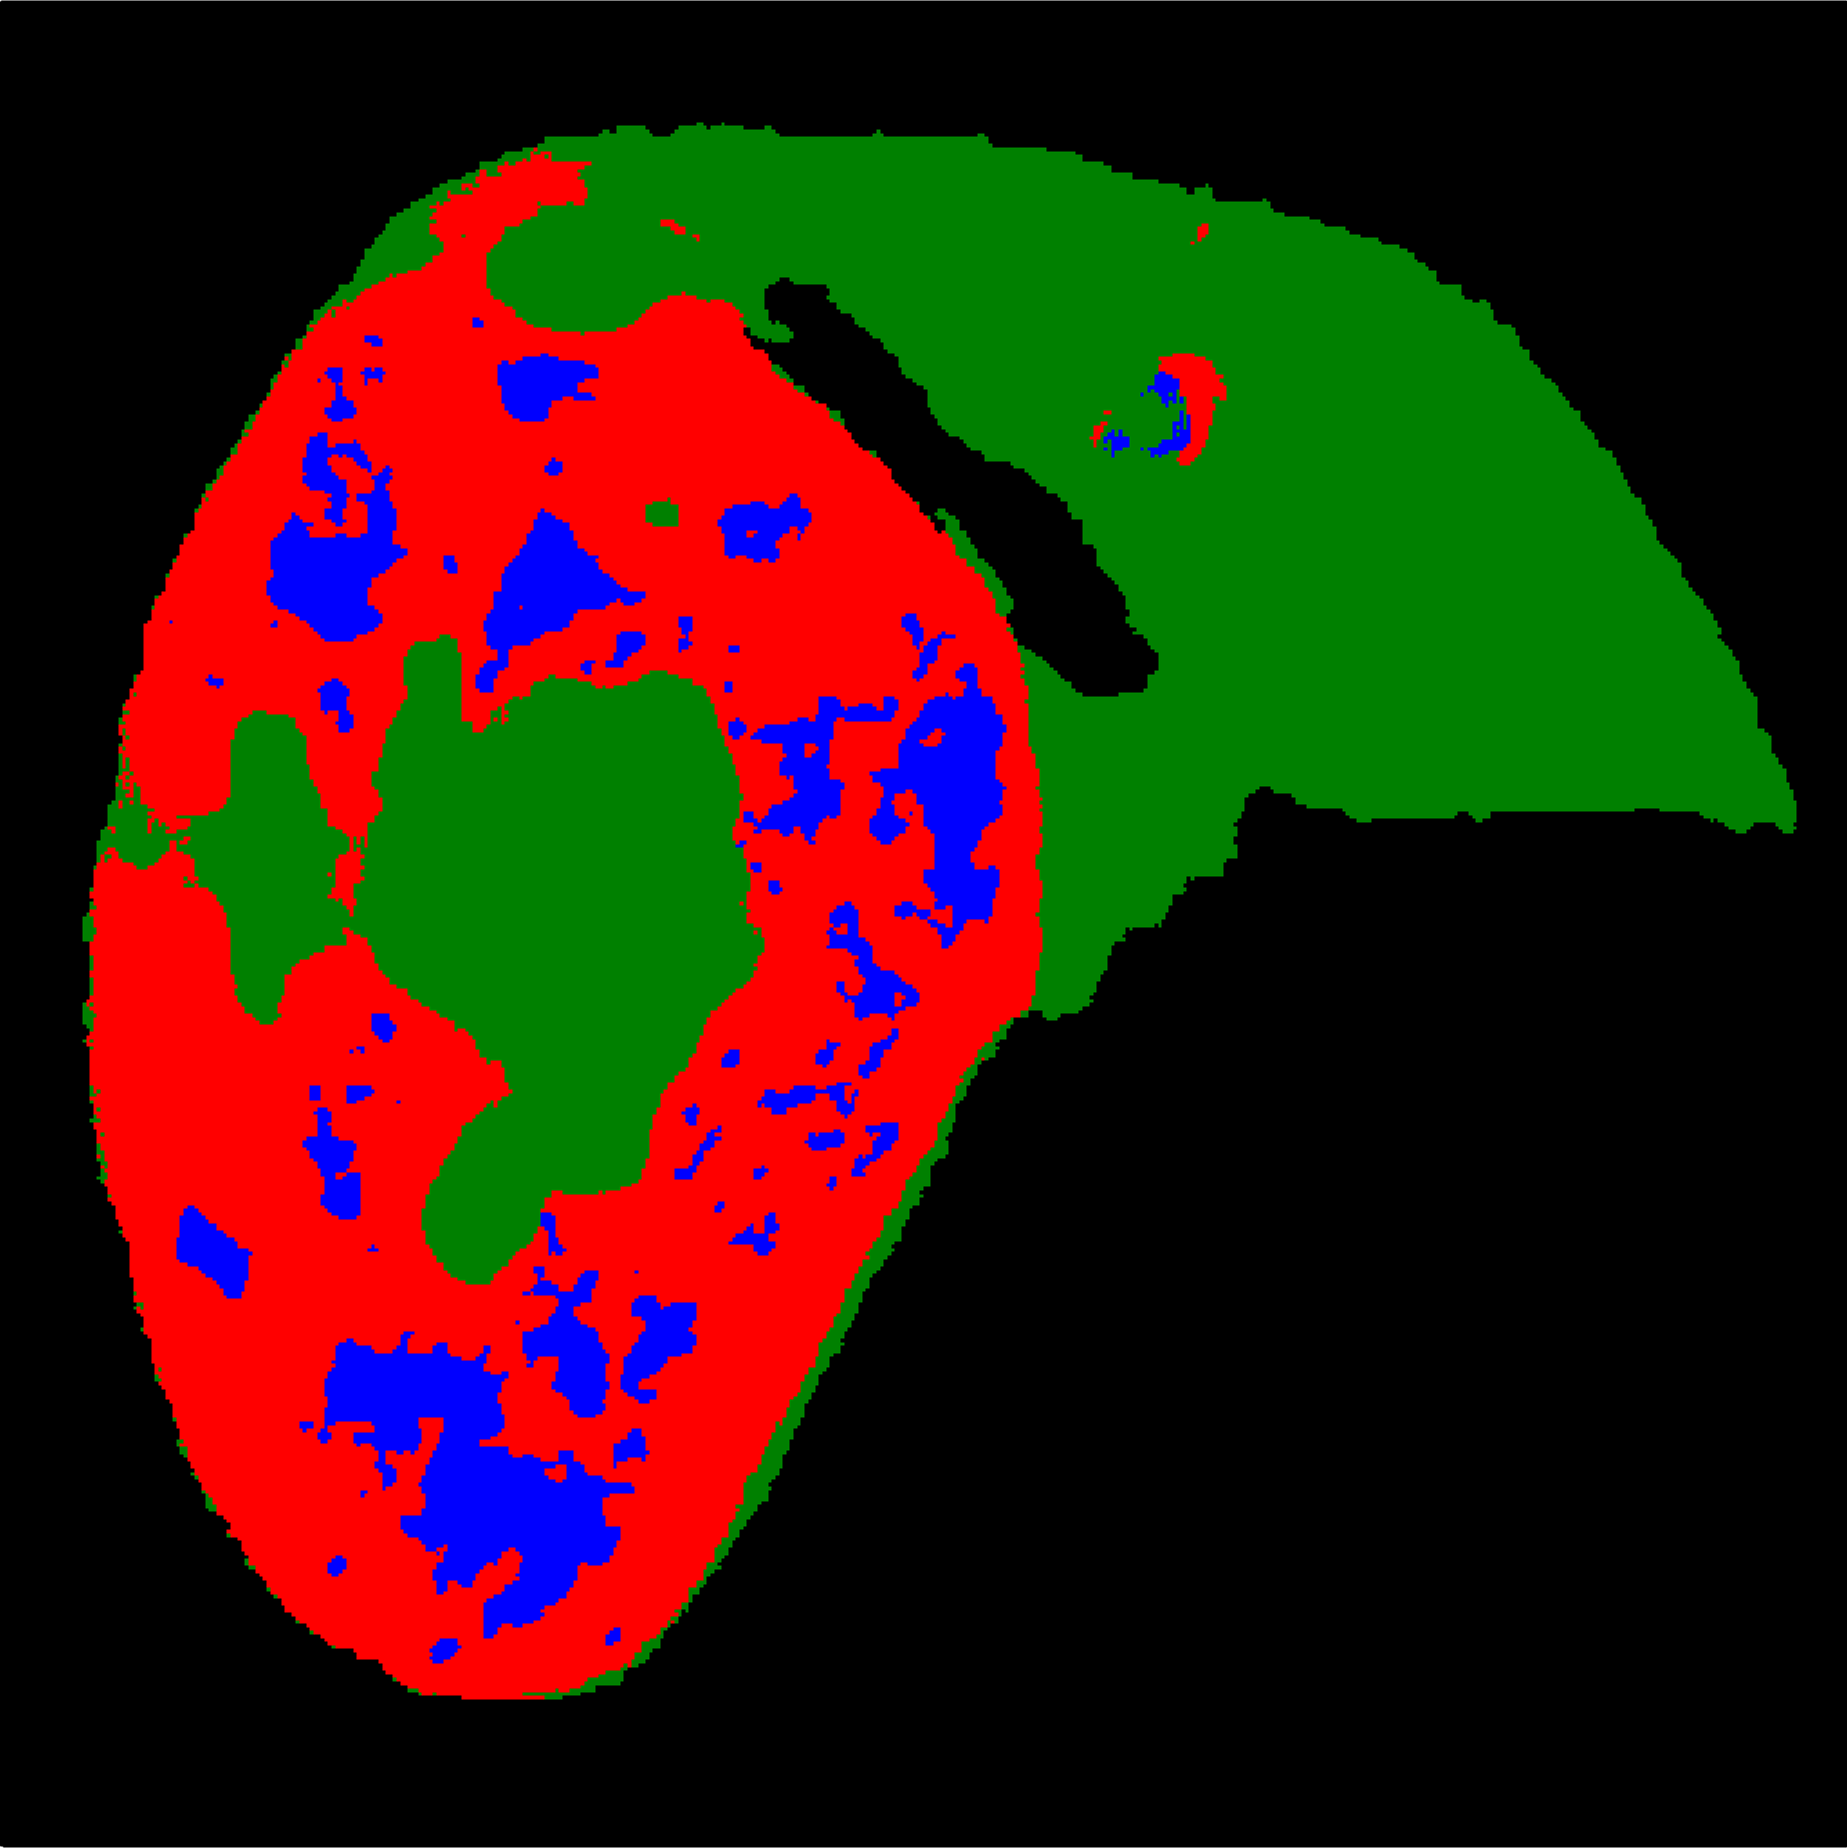
\includegraphics[width=\linewidth]{../SemanticSeg/images/5_8_FullDMP_resized}
\end{minipage} 
\vspace{-0.2cm}
\begin{minipage}{4cm}
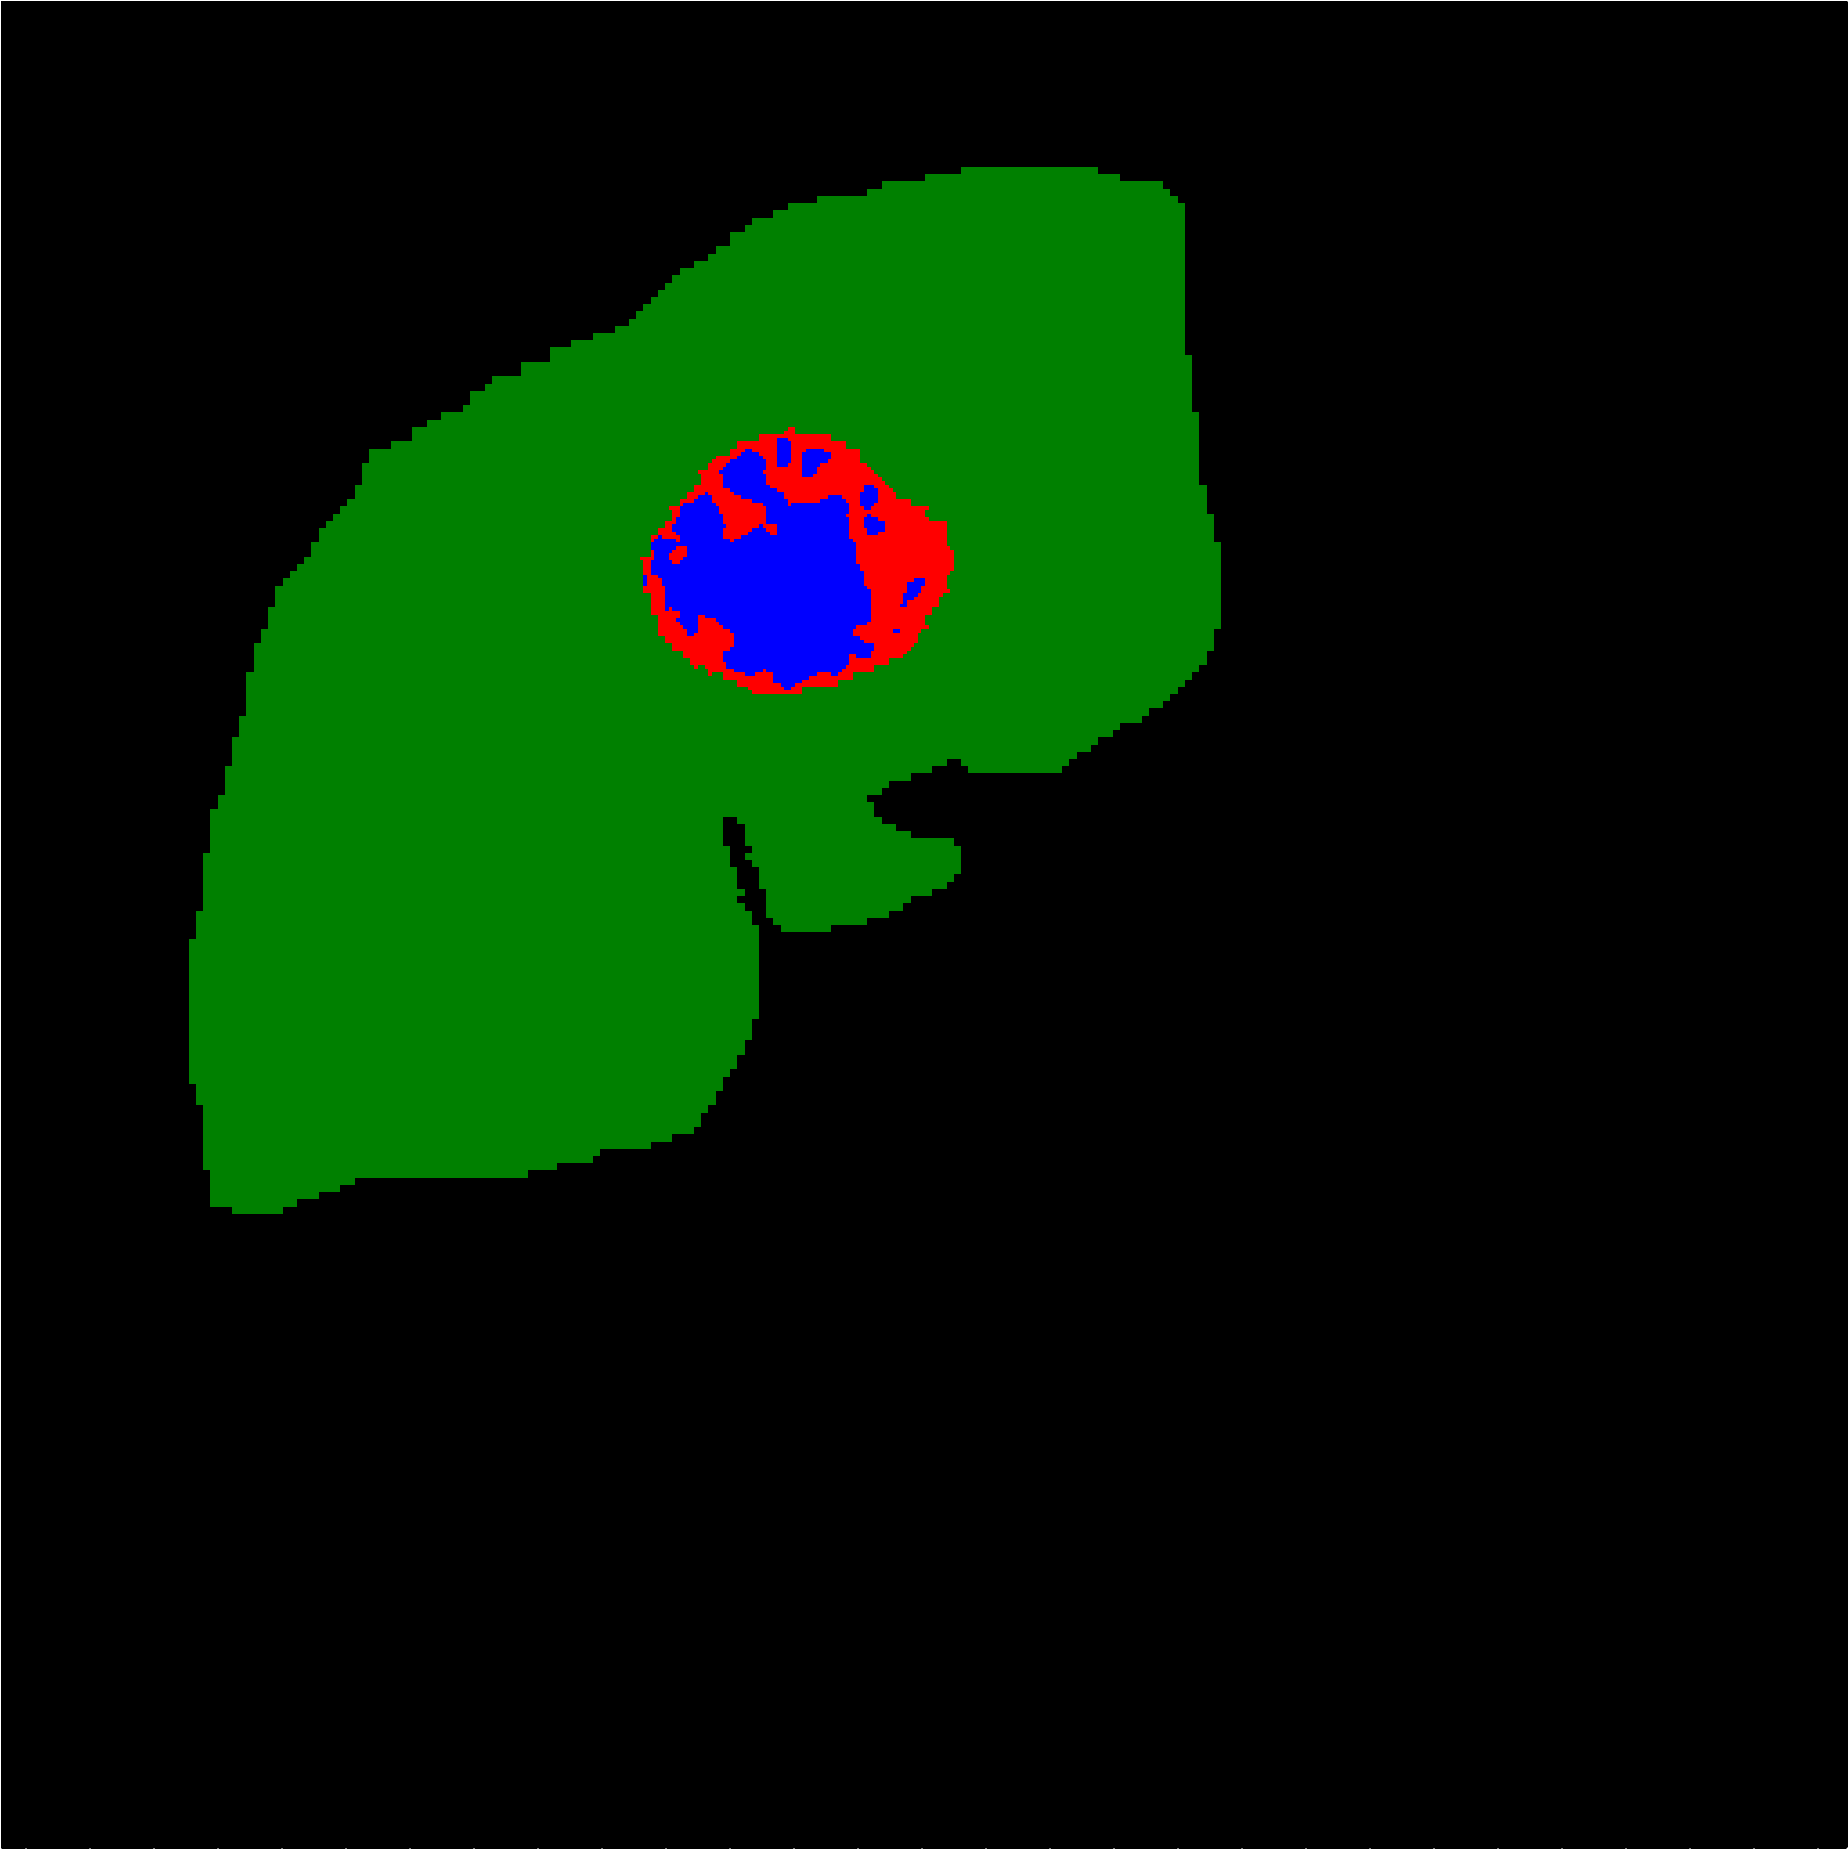
\includegraphics[width=\linewidth]{../SemanticSeg/images/1_21_Cascade_resized}
\end{minipage} \hspace{-0.3cm}
\begin{minipage}{4cm}
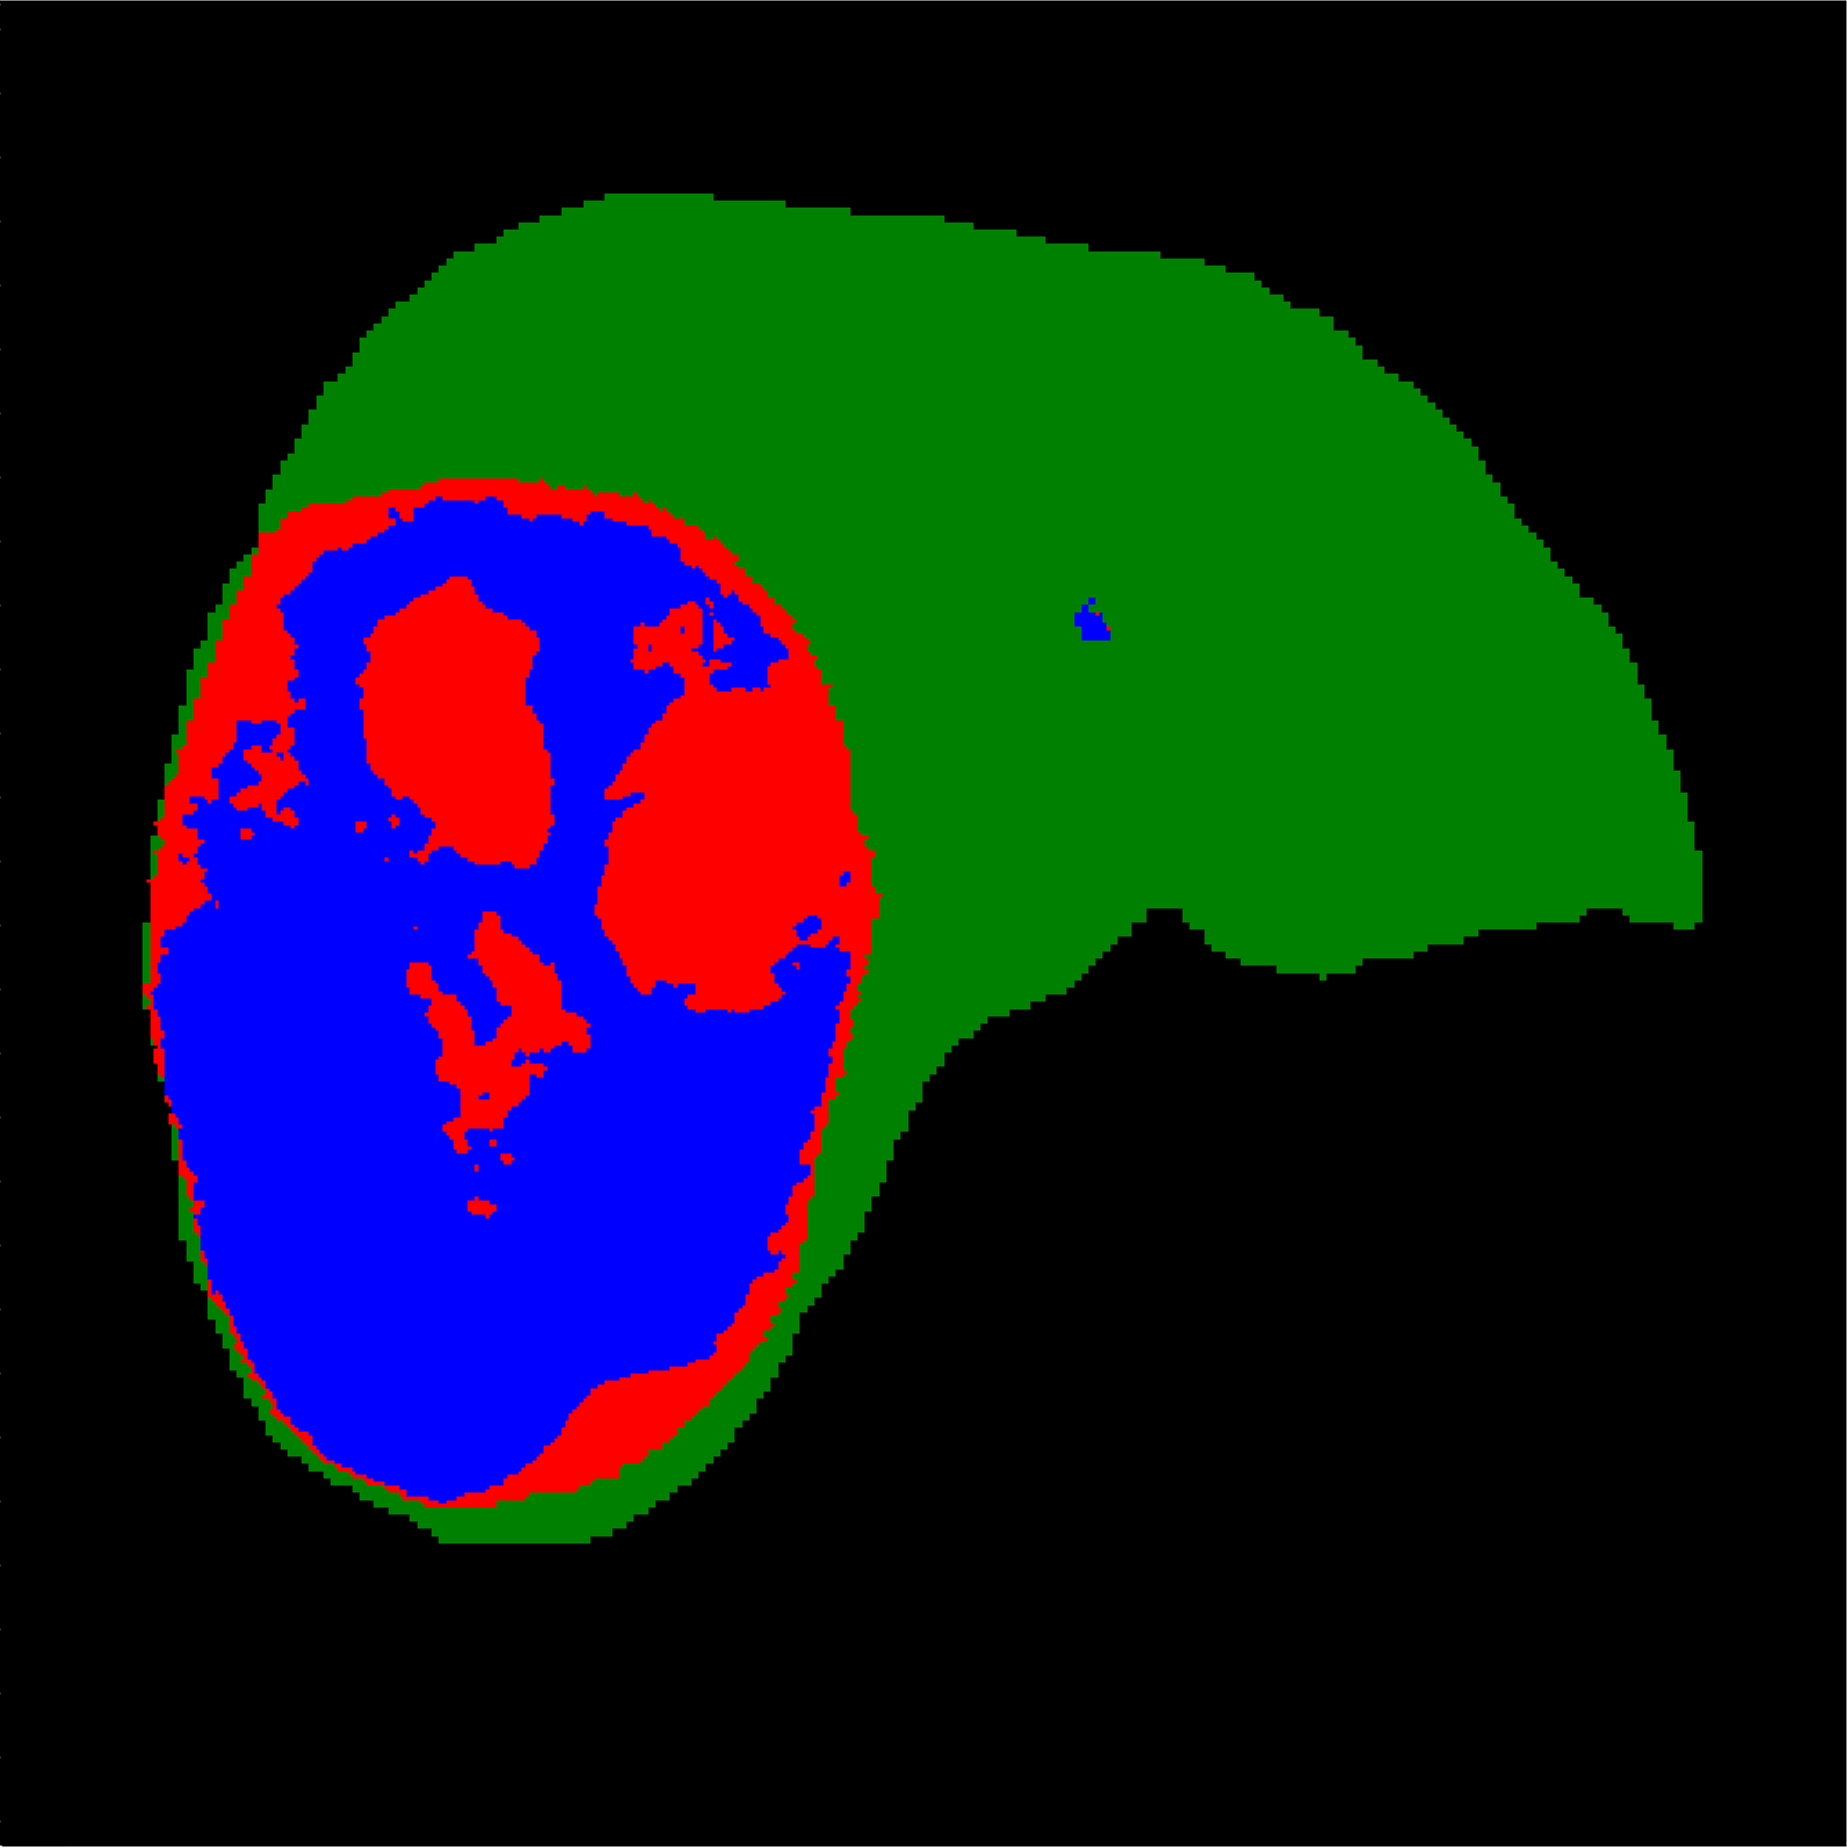
\includegraphics[width=\linewidth]{../SemanticSeg/images/5_2_Cascade_resized}
\end{minipage} \hspace{-0.3cm}
\begin{minipage}{4cm}
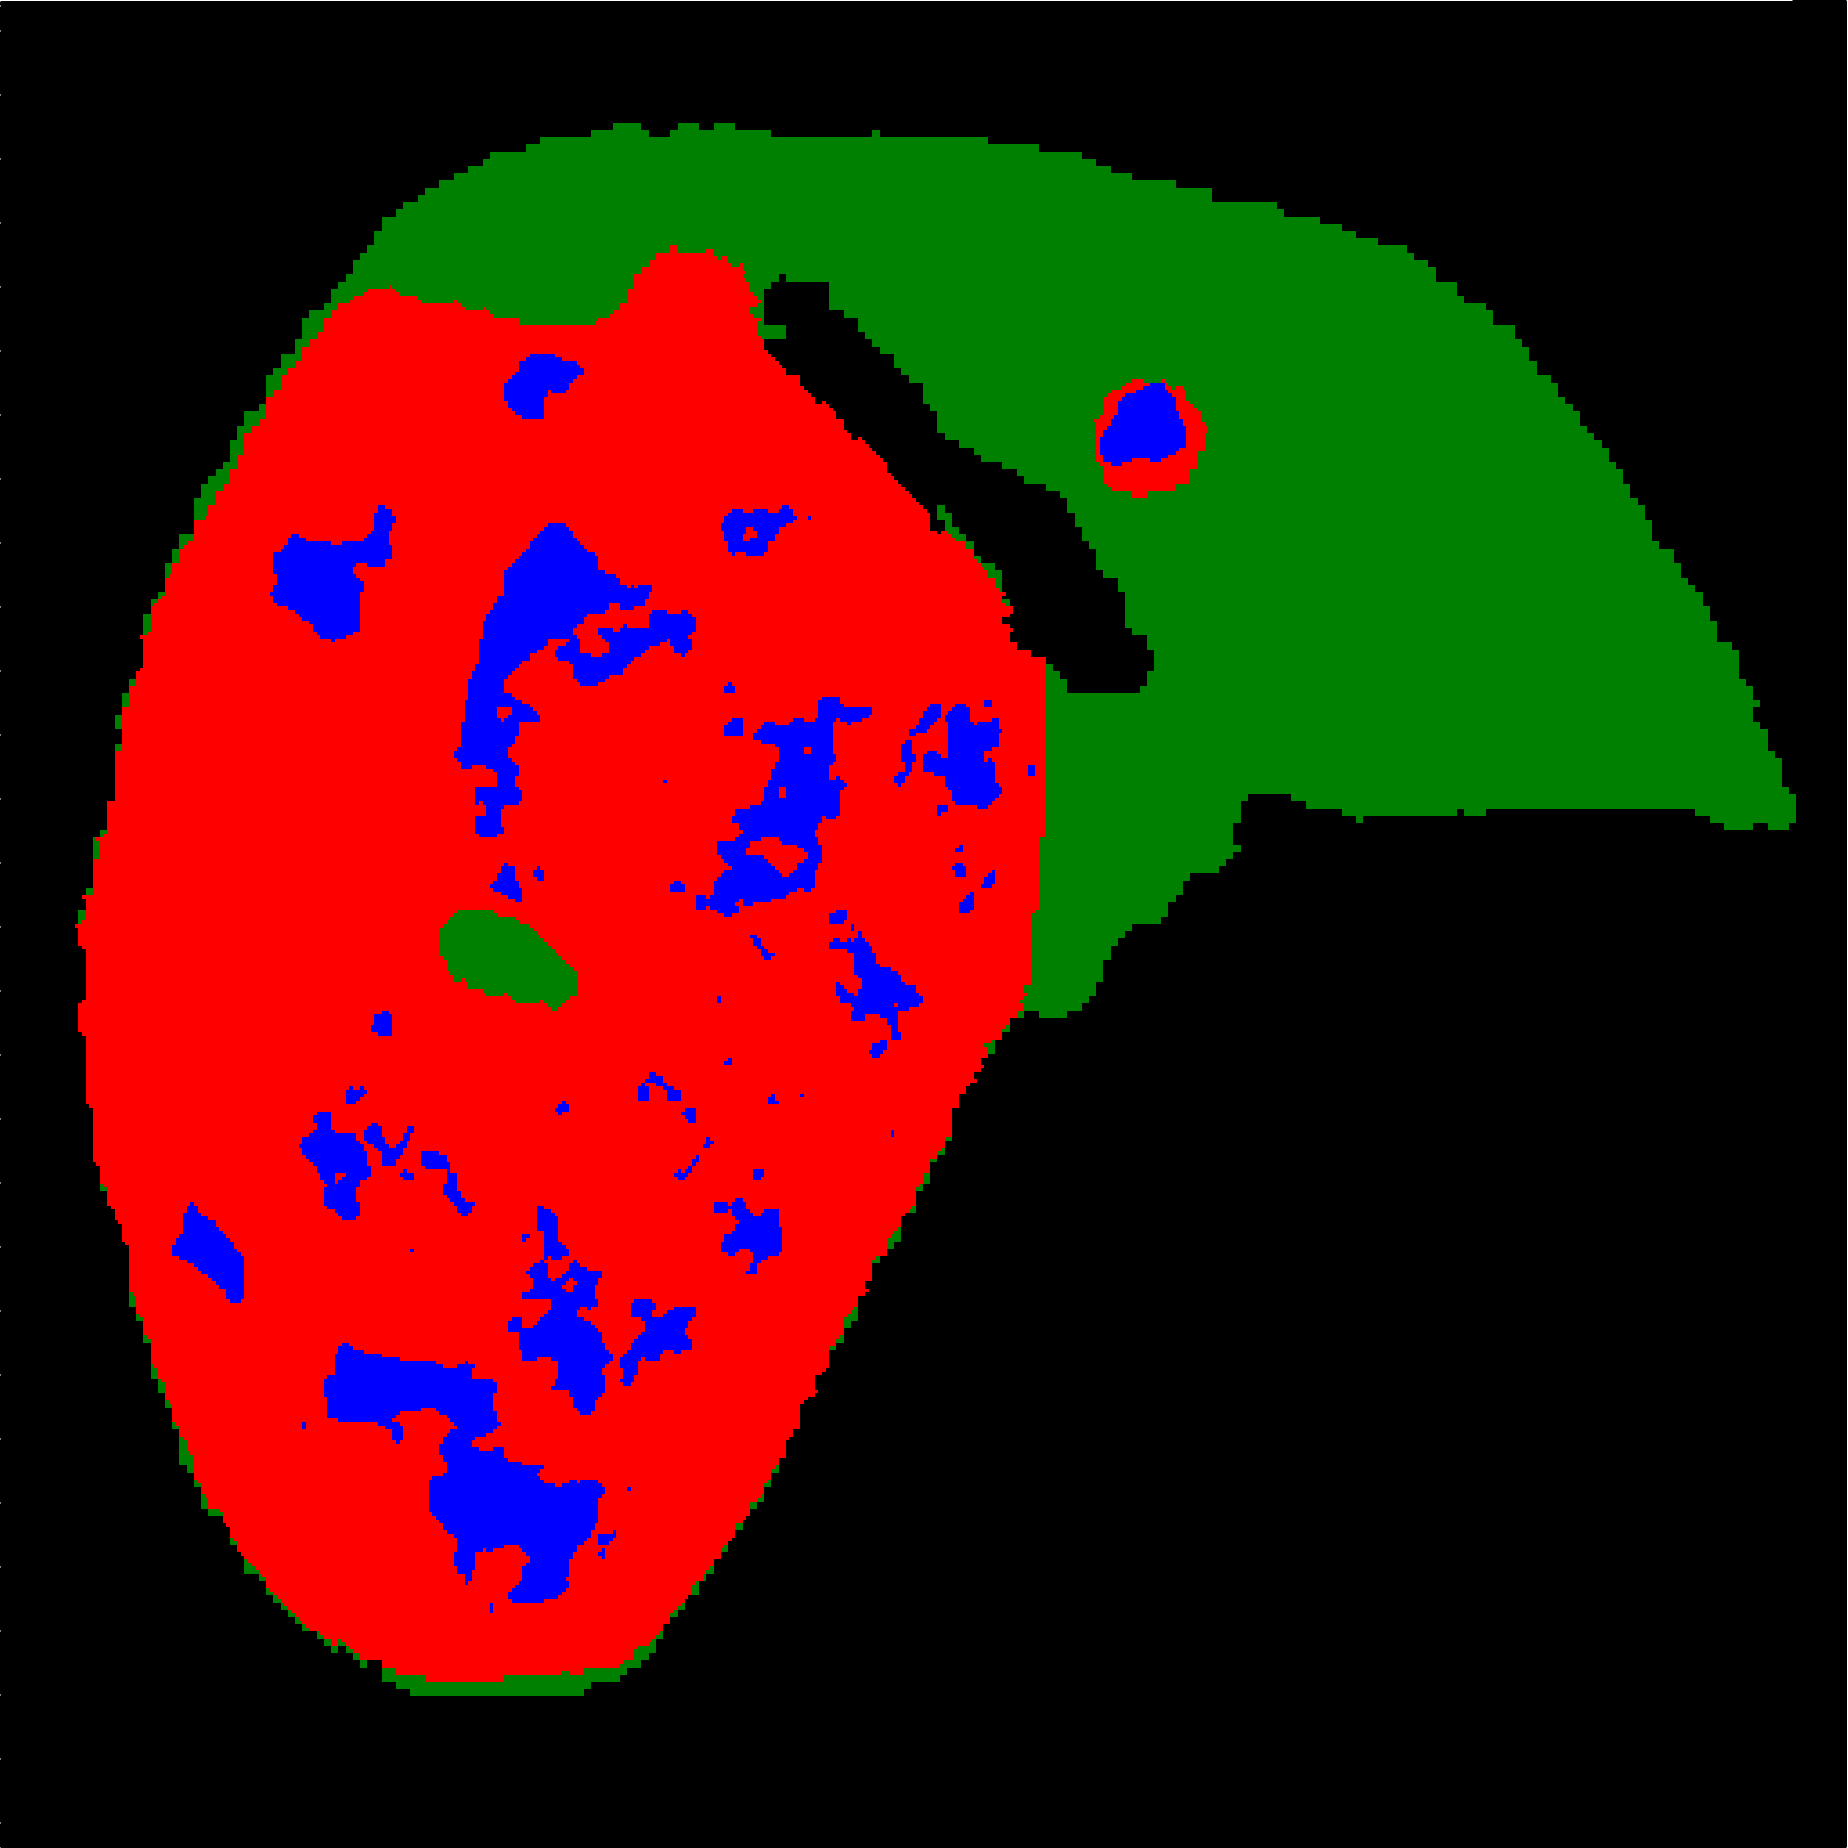
\includegraphics[width=\linewidth]{../SemanticSeg/images/5_8_Cascade_resized}
\end{minipage} 
\caption{From top to bottom : Raw images with HU values inside the liver, Ground truth, \pplfont{DMP-Full} segmentation, Cascaded DMP segmentation}
\label{CompareFullCascade}
\end{figure}


We finally combined the \pplfont{DMP-Liver}, the \pplfont{DMP-Lesion} and \pplfont{DMP-Necrosis} networks in a cascaded fashion, as described in the figure \ref{CARS_Cascade}. This allowed us to perform a fully automatic segmentation of the raw (unmasked) \ac{ct} images. We reached average slice-wise \ac{dsc}s of 78.3 $\pm$ 22.1 for the segmentation of the parenchyma, 50.6 $\pm$ 24.6  for the segmentation of the active part, and 68.1 $\pm$ 23.2 for the necrotic part of the lesions. We also provided a necrosis rate per patient with a mean error of 15.9\% when compared to expert necrosis rate estimation \footnote{Here the estimation is performed on the raw images in an automatic fashion}. Examples of fully automatic segmentation results are given in figure \ref{FullAutoSeg}.

\begin{figure}[!ht]
   \centering
\begin{minipage}{4cm}
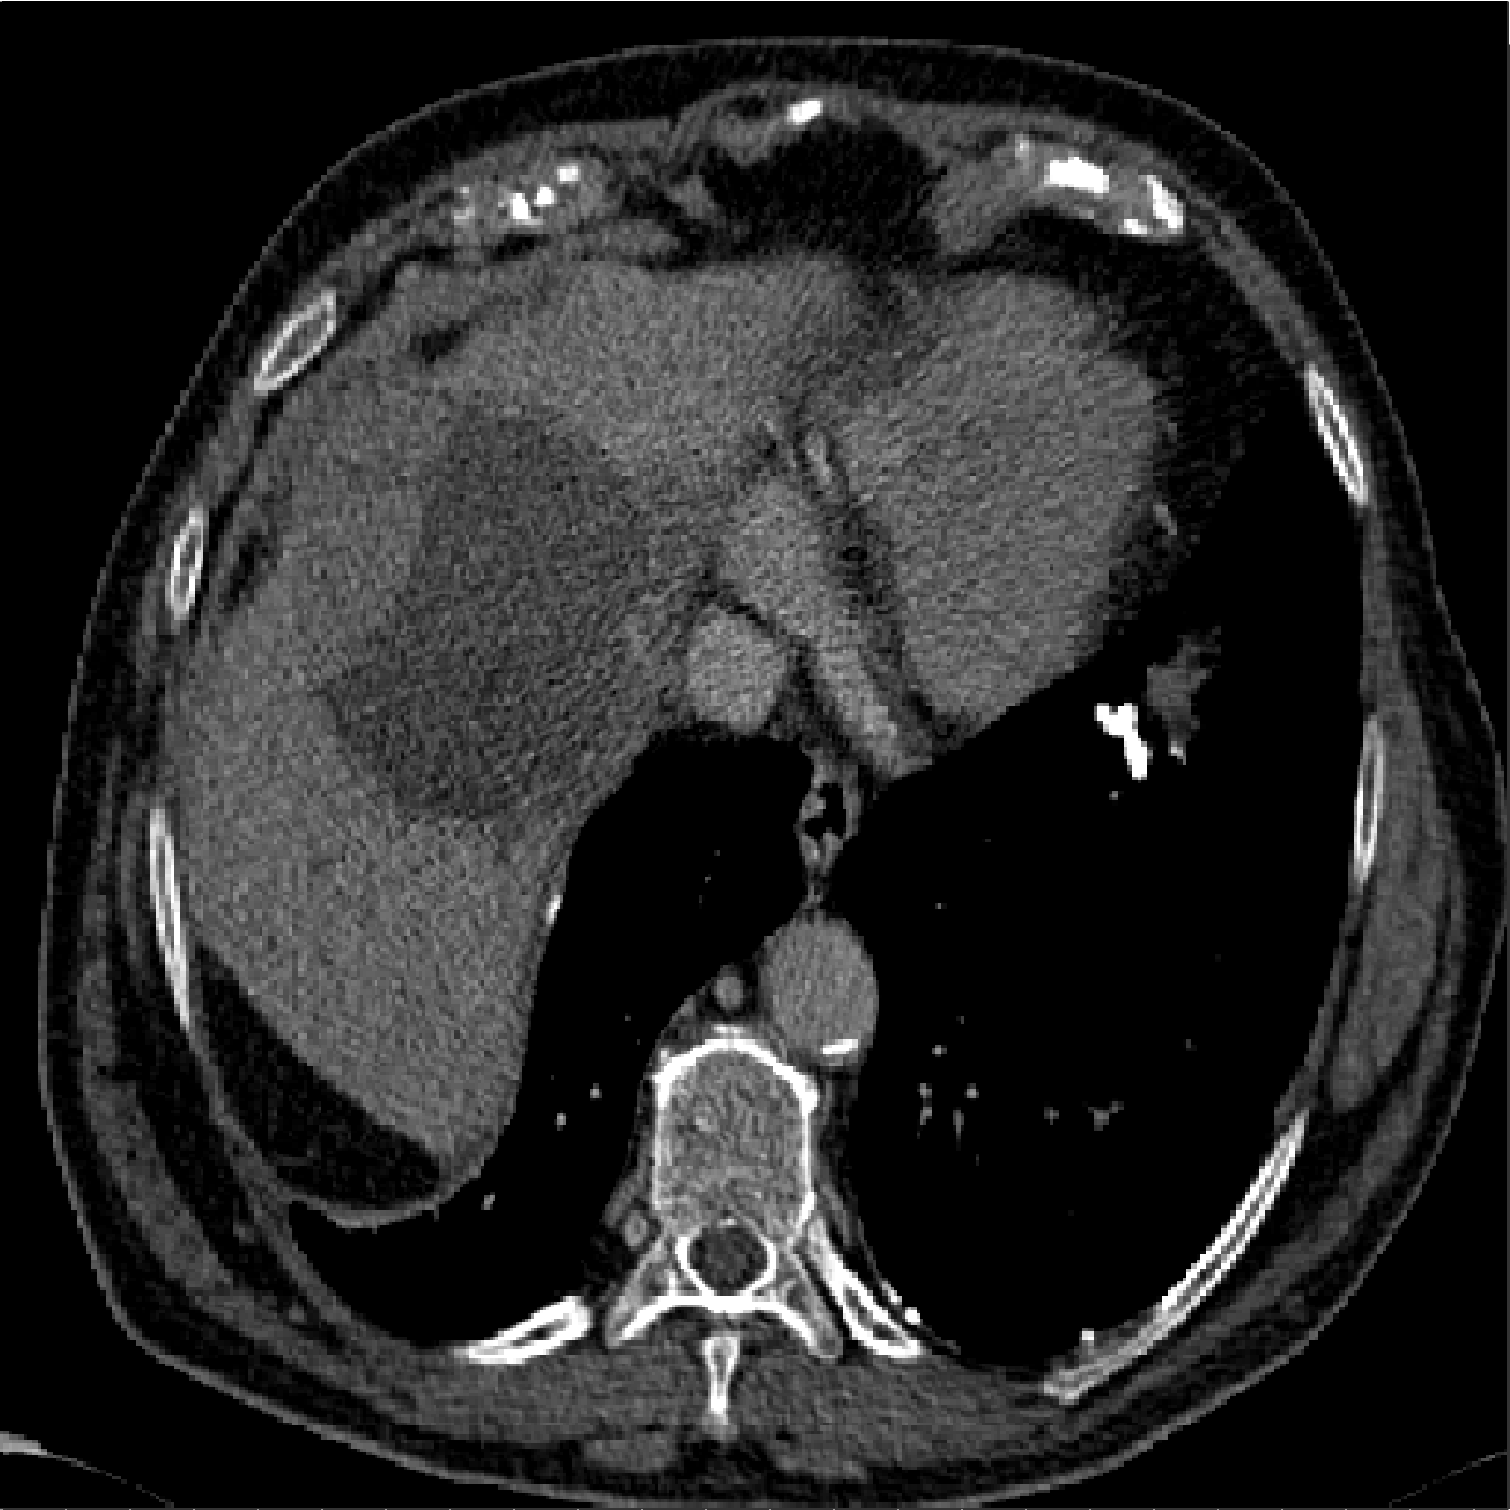
\includegraphics[width=\linewidth]{../SemanticSeg/images/1_7_raw_new_resized}
\end{minipage} \hspace{-0.3cm}
\begin{minipage}{4cm}
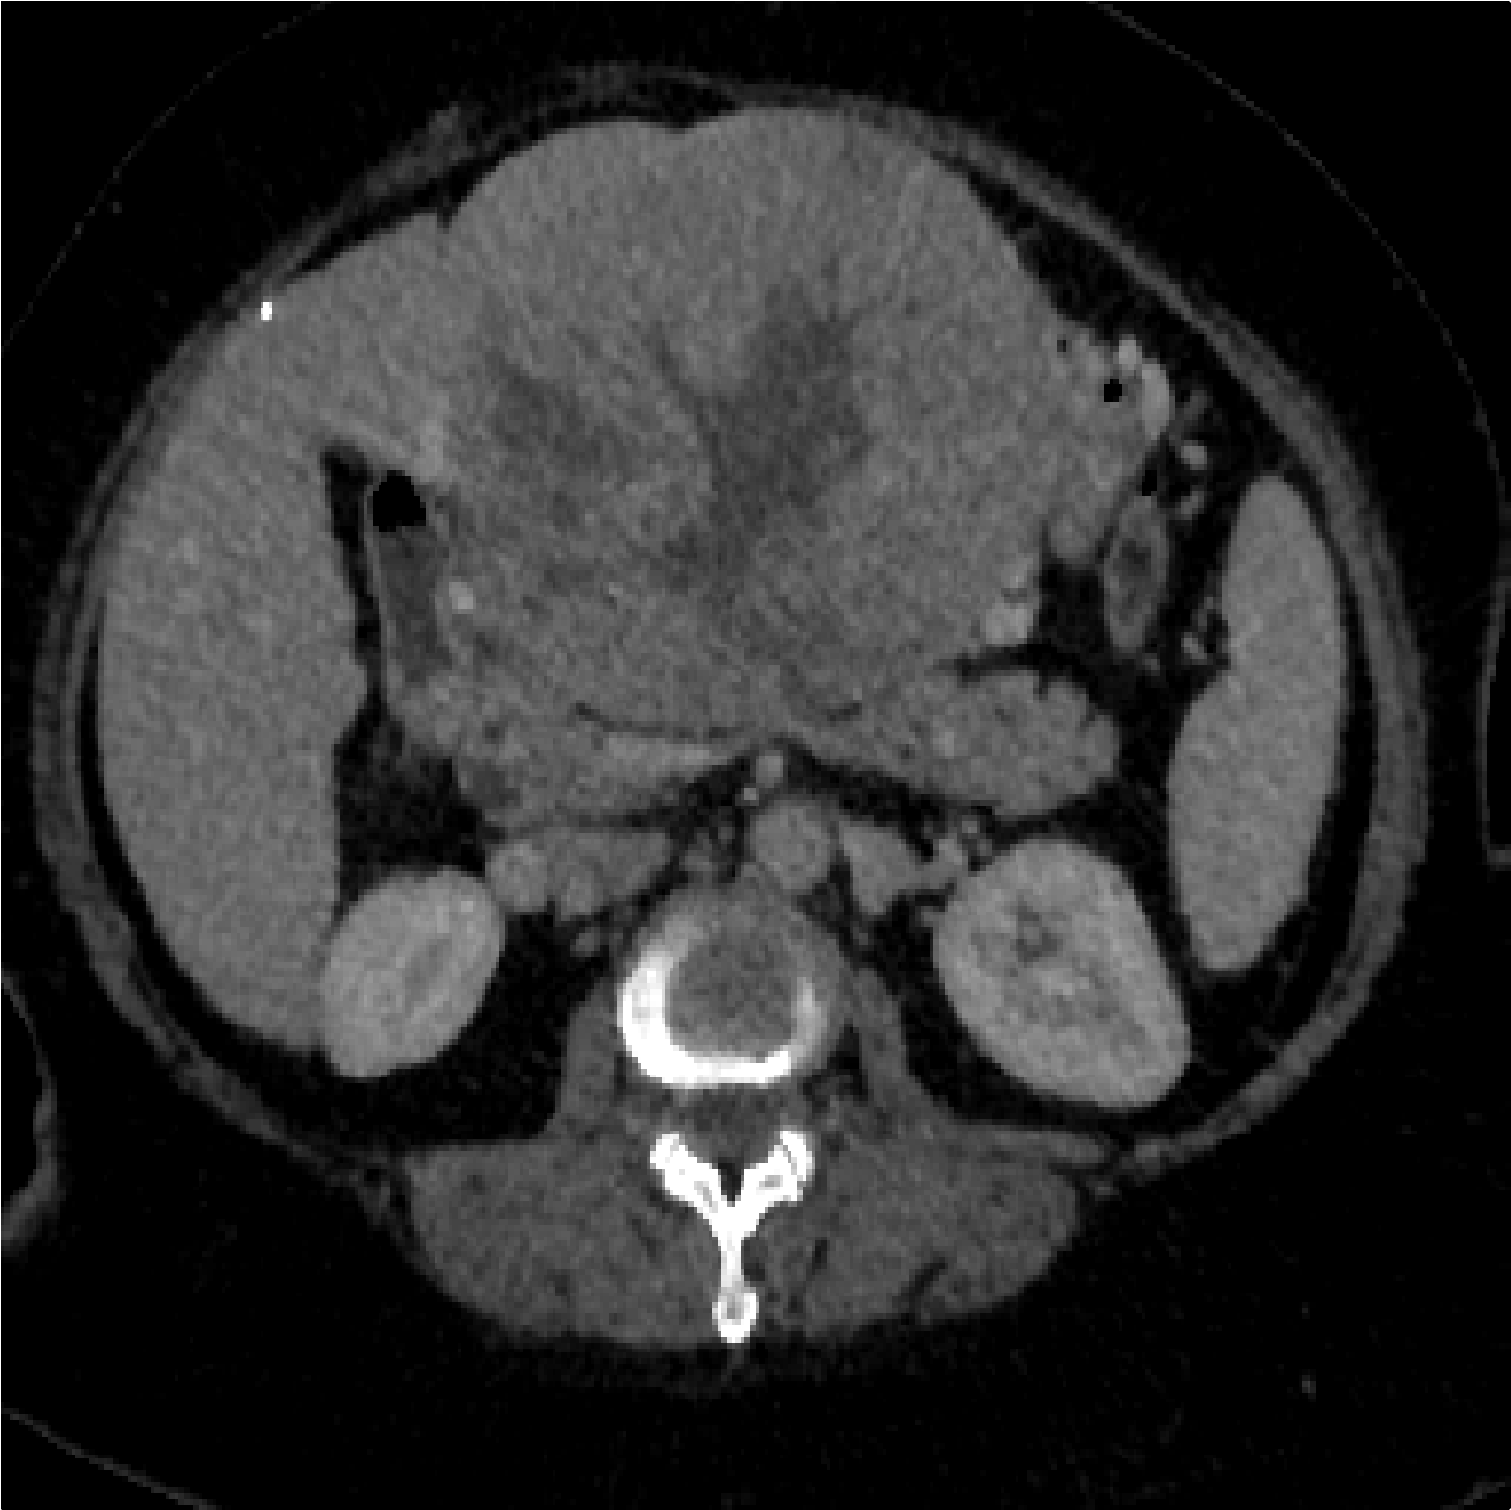
\includegraphics[width=\linewidth]{../SemanticSeg/images/2_3_raw_resized}
\end{minipage} \hspace{-0.3cm}
\begin{minipage}{4cm}
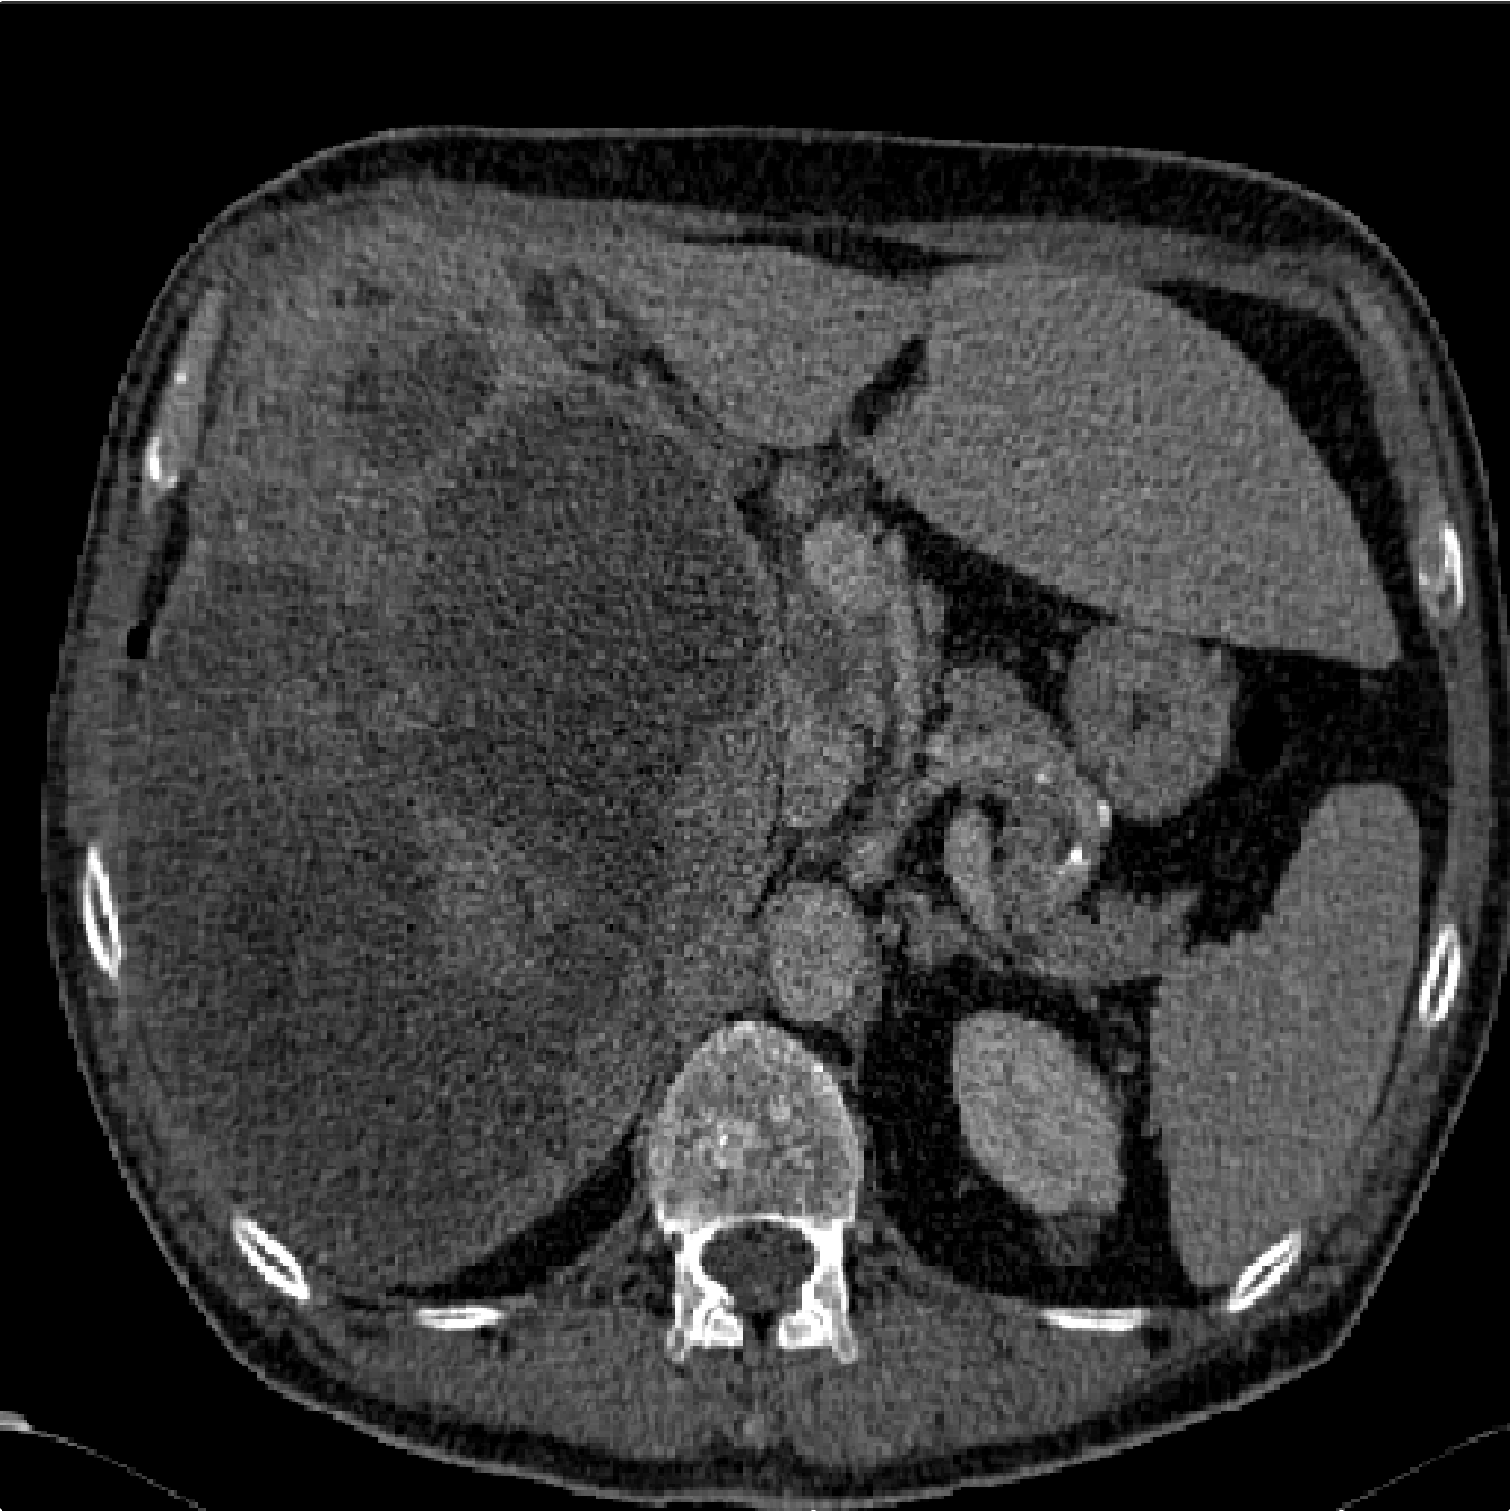
\includegraphics[width=\linewidth]{../SemanticSeg/images/5_4_raw_resized}
\end{minipage}
\vspace{-0.2cm}
\begin{minipage}{4cm}
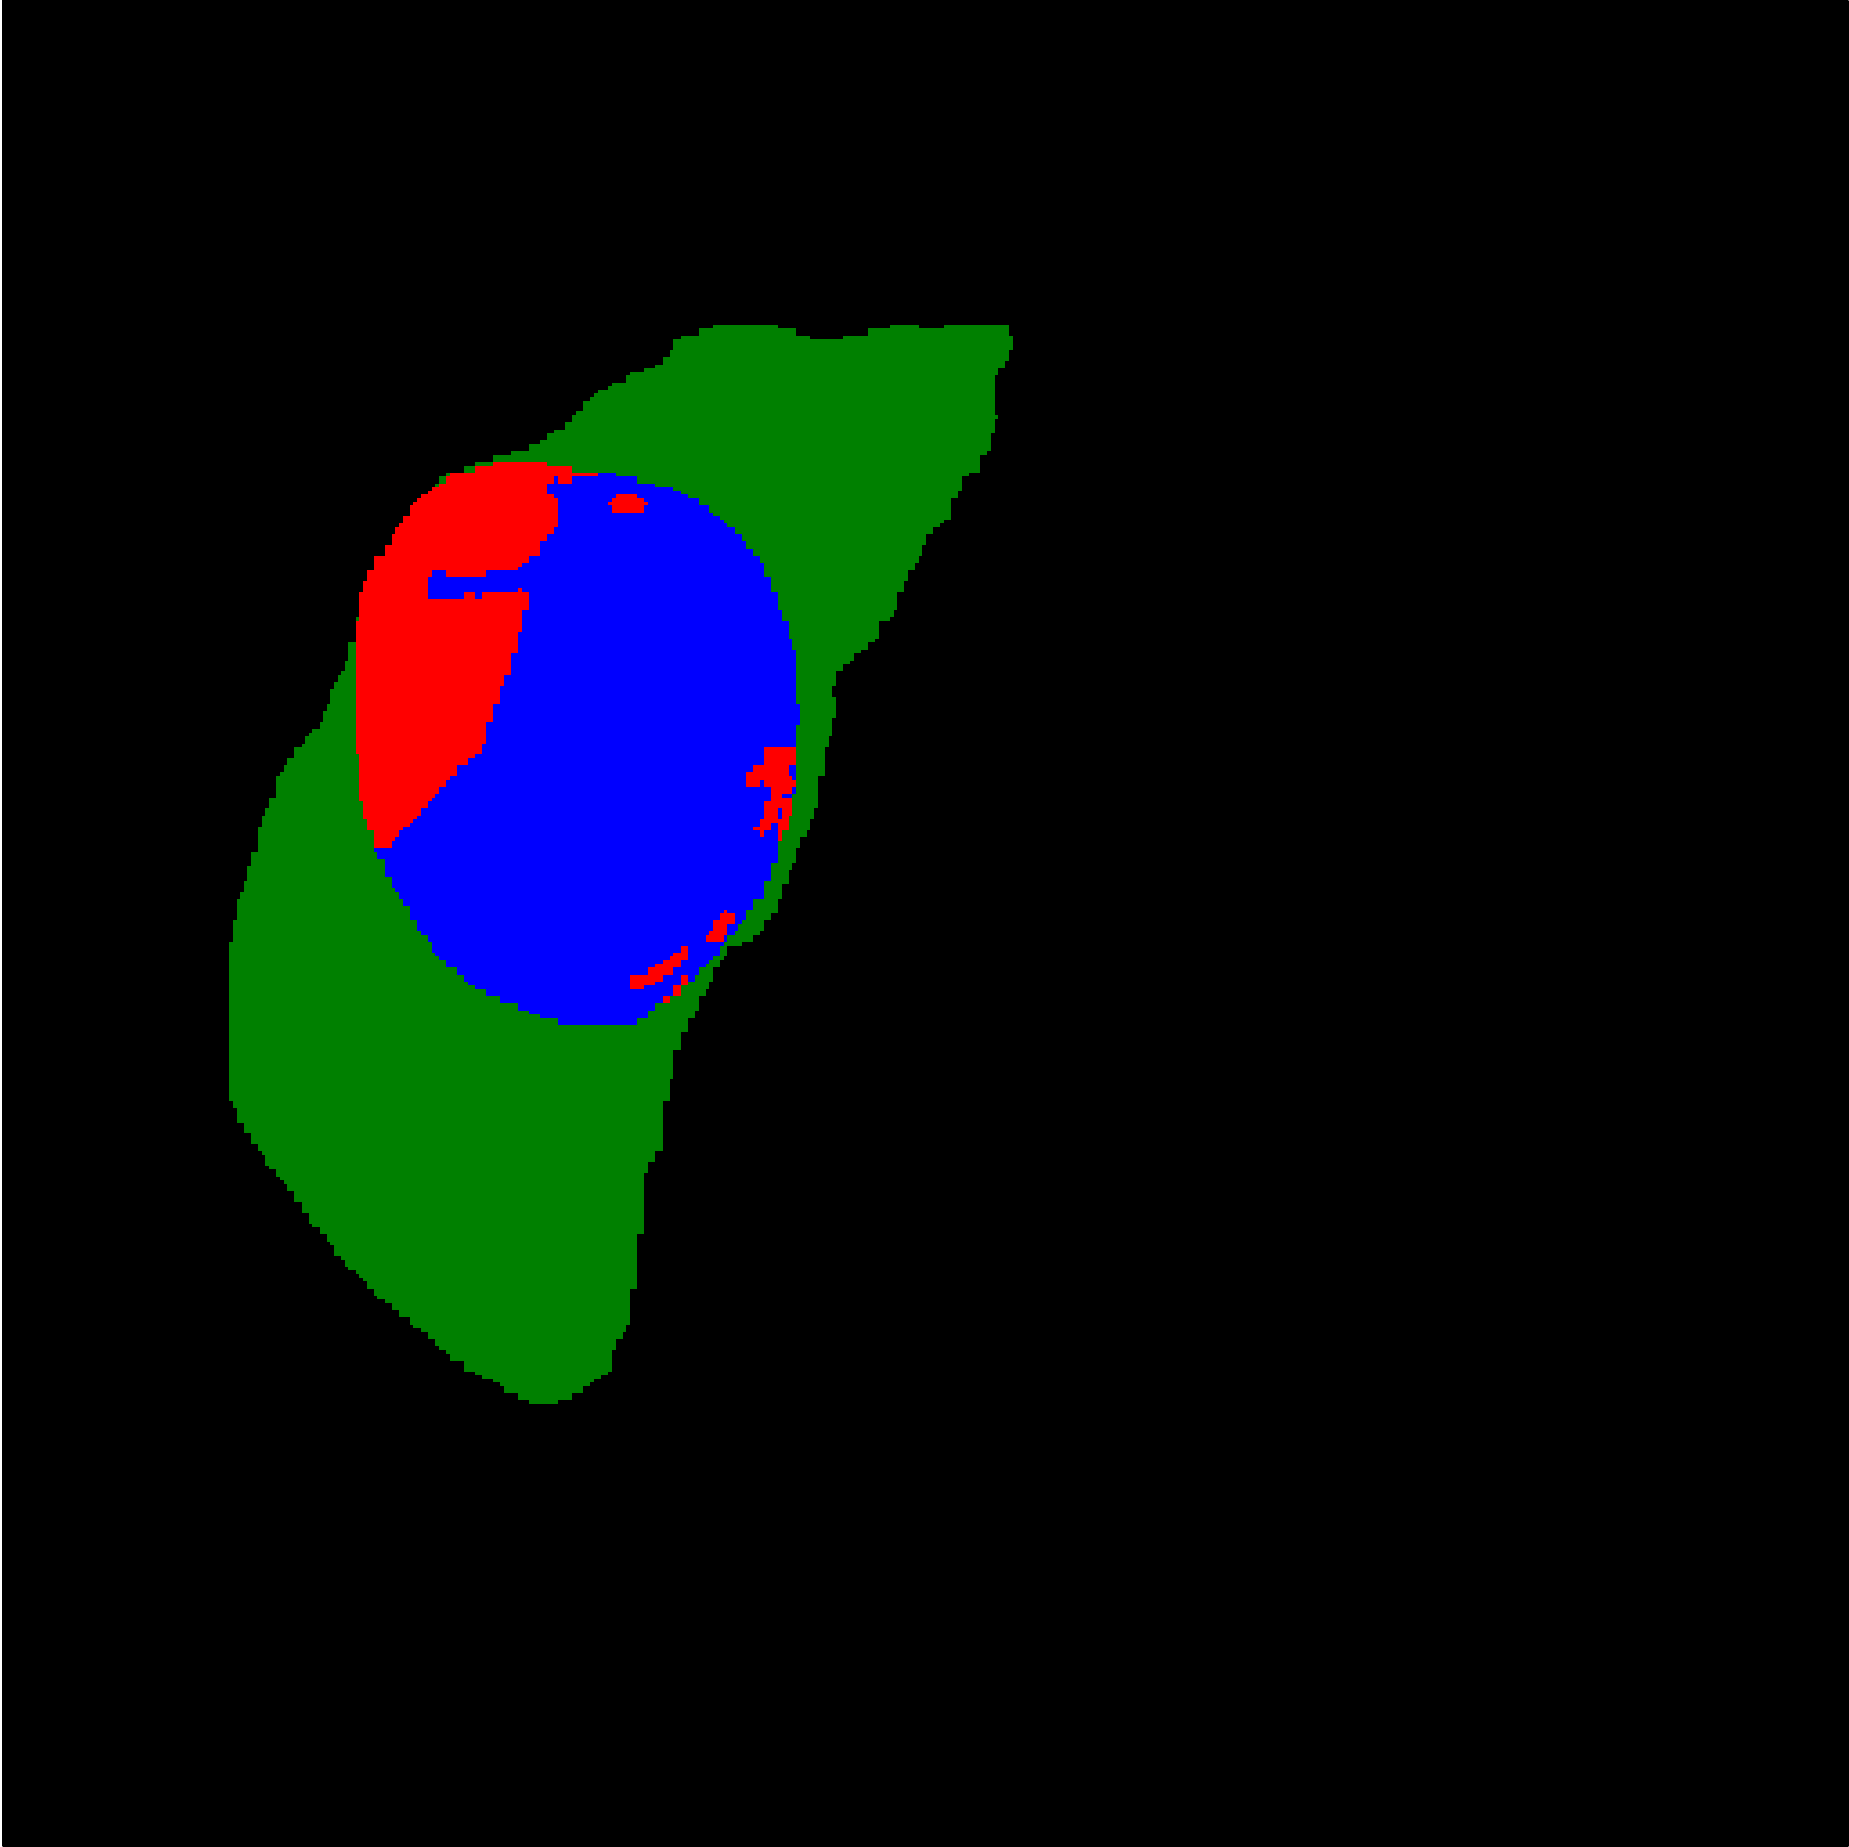
\includegraphics[width=\linewidth]{../SemanticSeg/images/1_7_gt_new_resized}
\end{minipage} \hspace{-0.3cm}
\begin{minipage}{4cm}
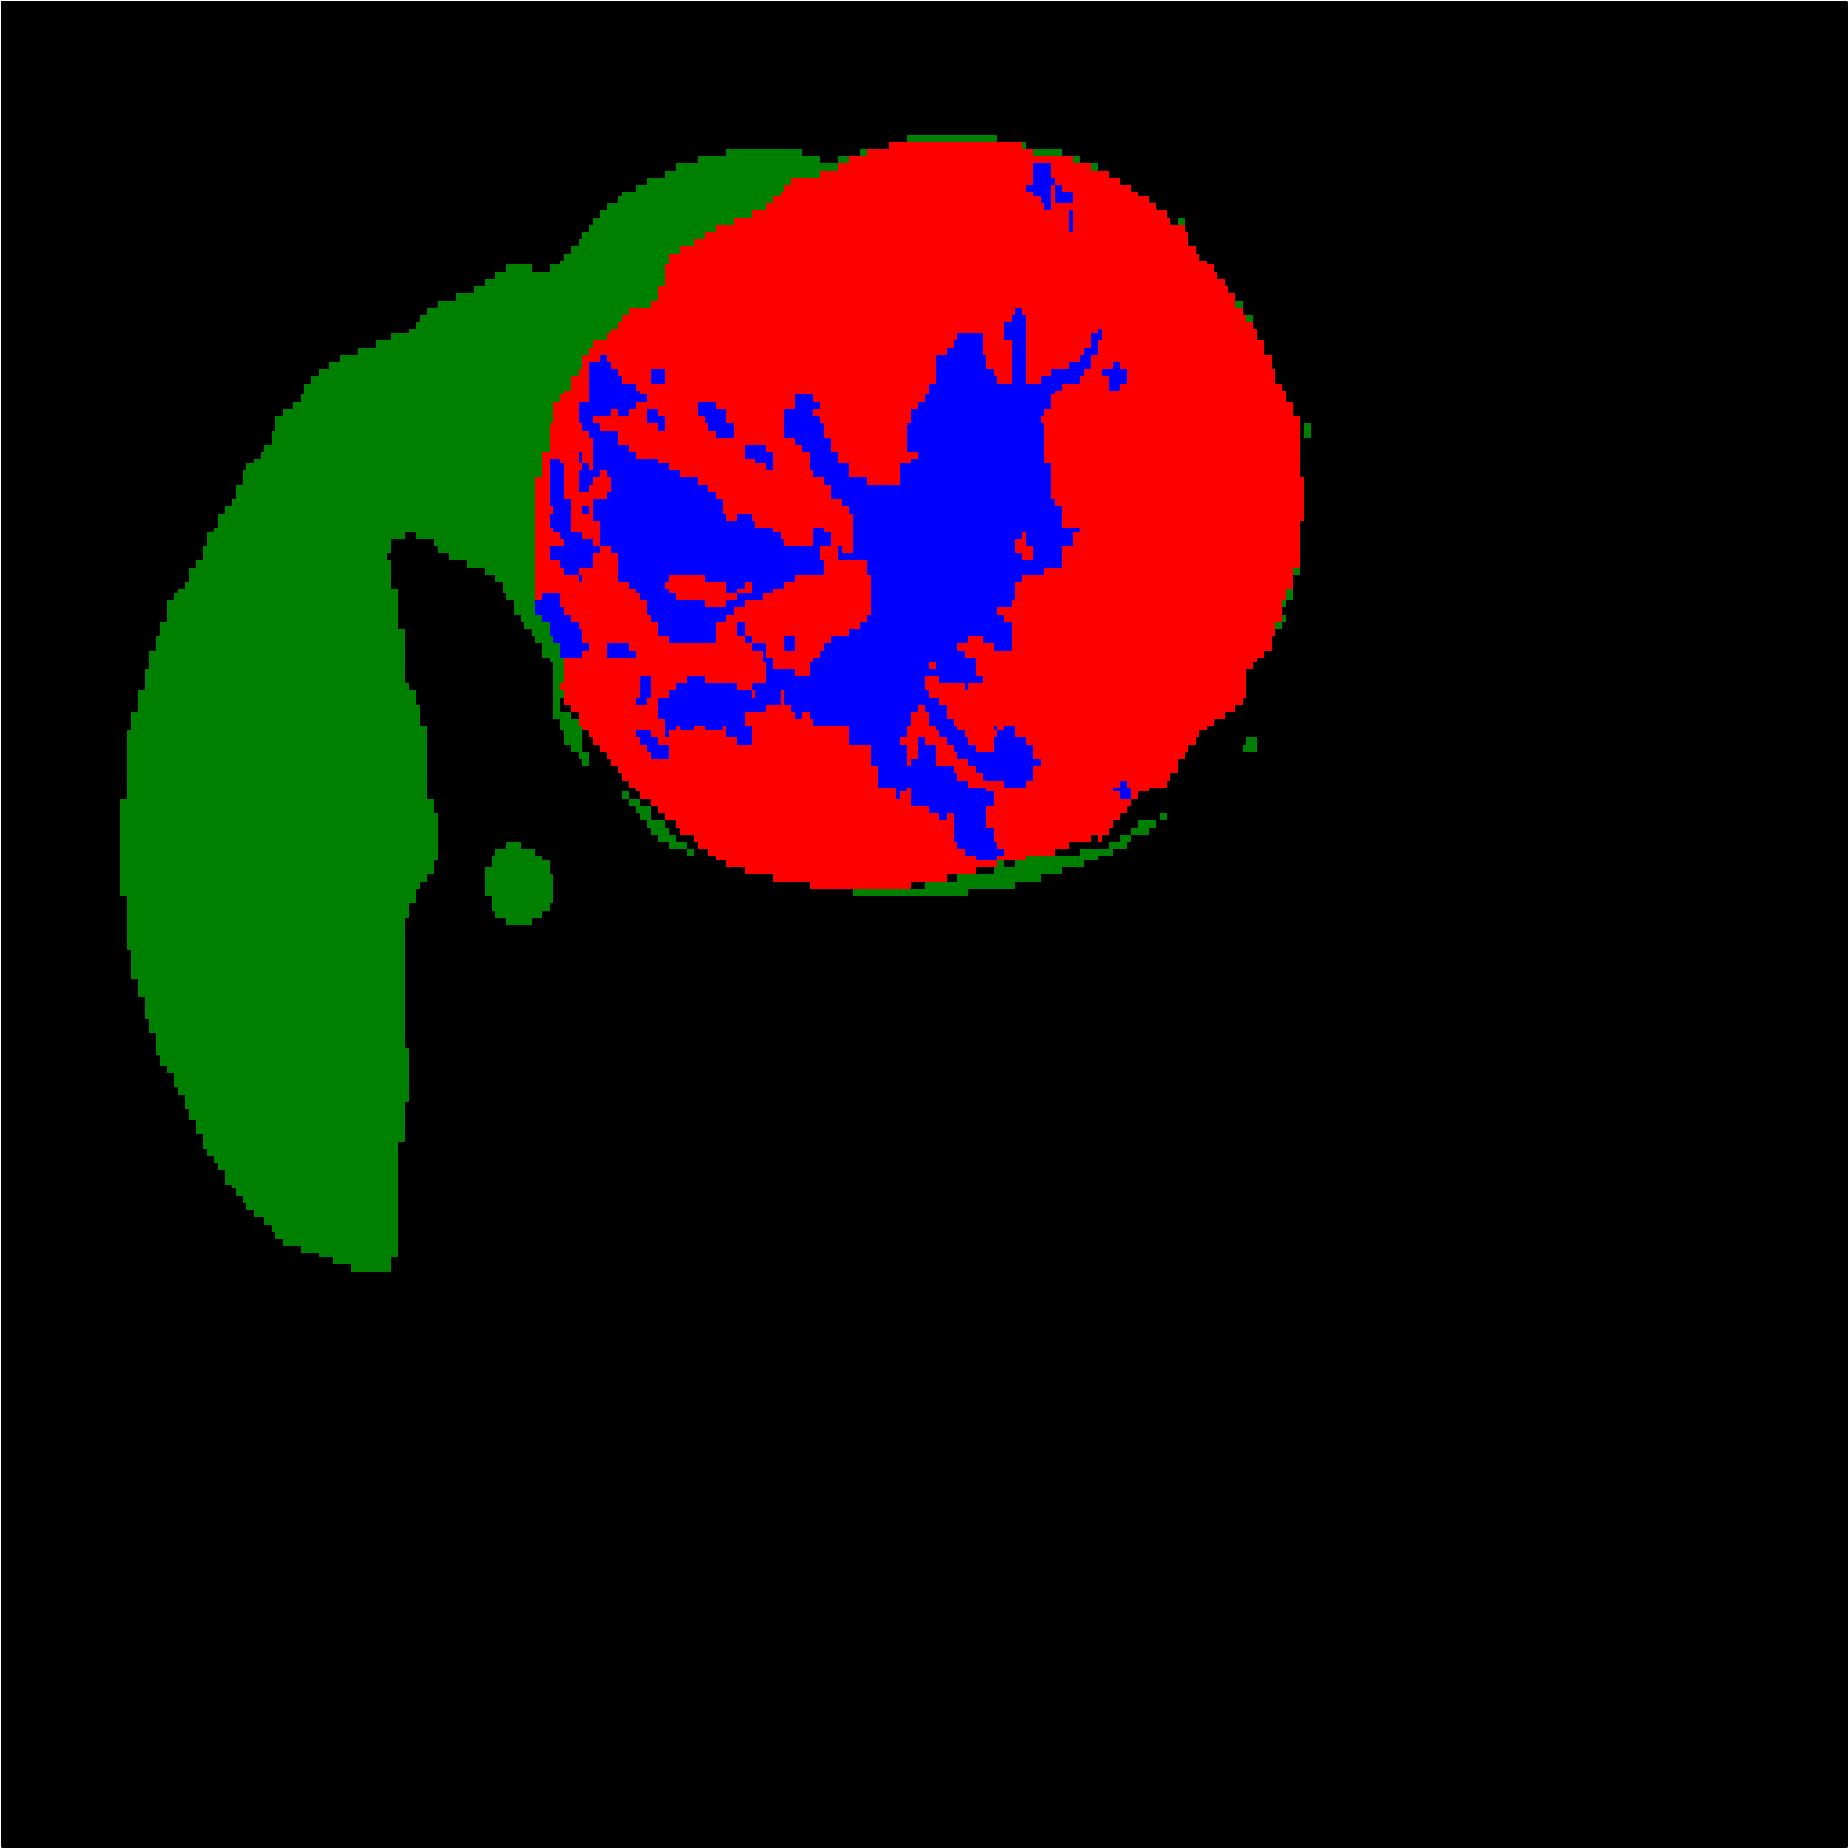
\includegraphics[width=\linewidth]{../SemanticSeg/images/2_3gt_resized}
\end{minipage} \hspace{-0.3cm}
\begin{minipage}{4cm}
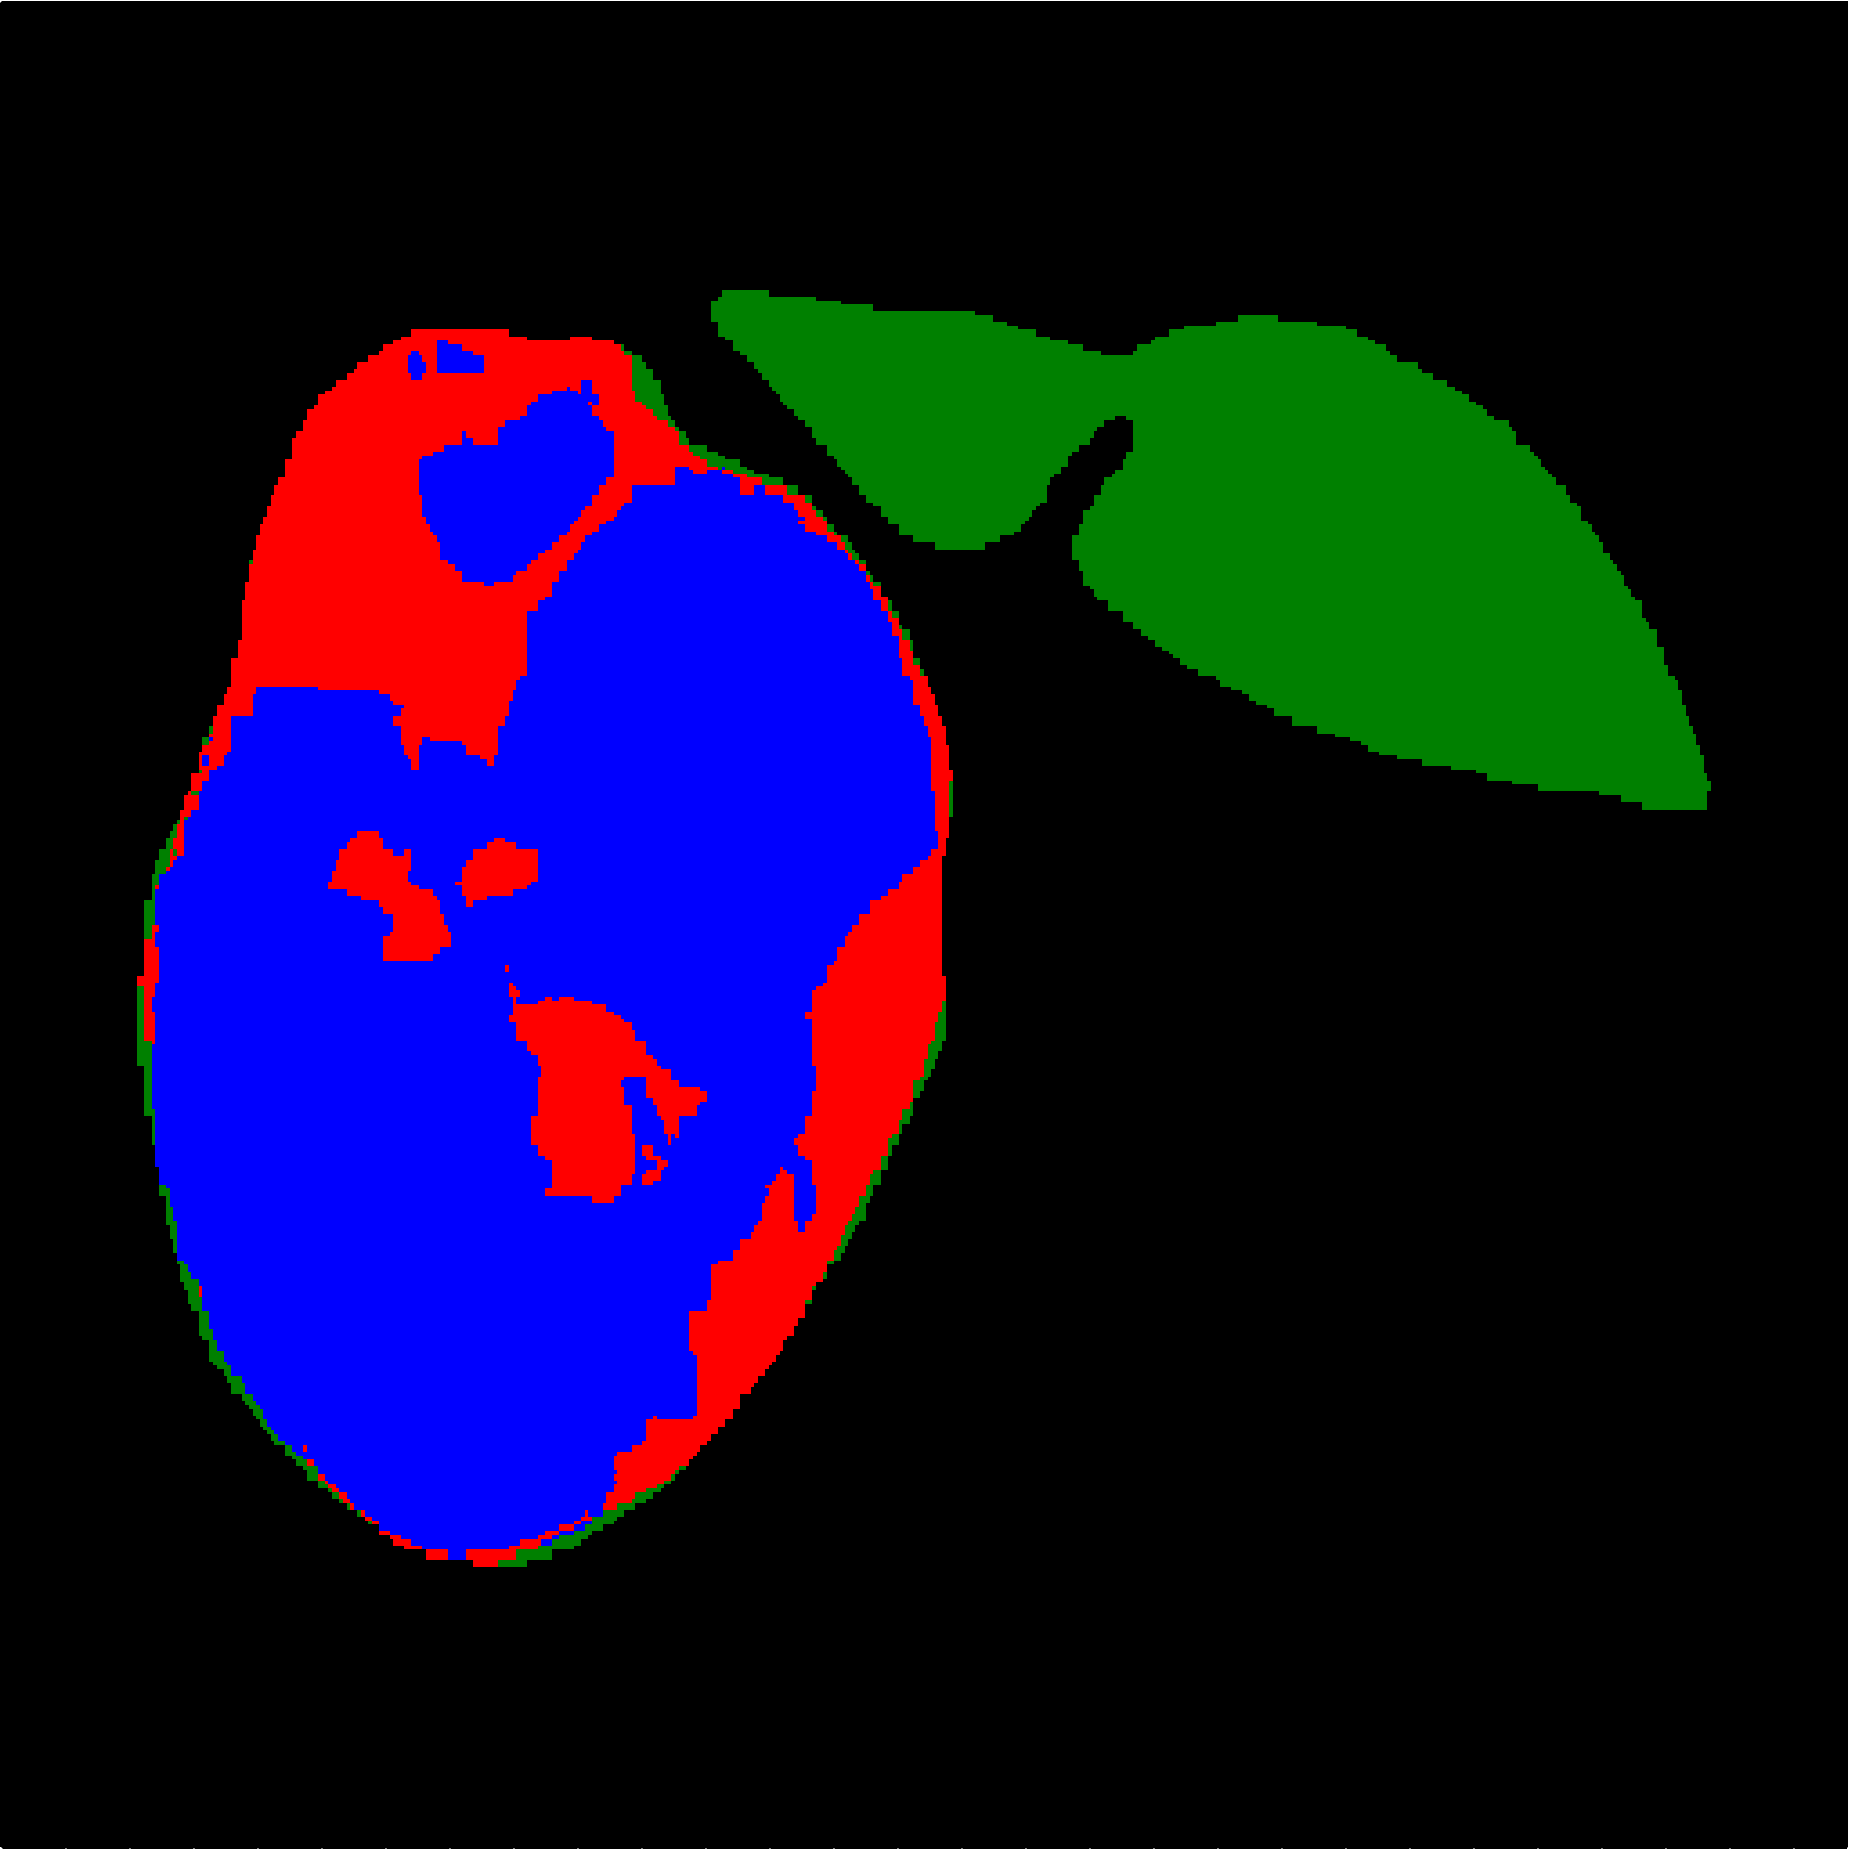
\includegraphics[width=\linewidth]{../SemanticSeg/images/5_4_gt_resized}
\end{minipage} 
\vspace{-0.2cm}
\begin{minipage}{4cm}
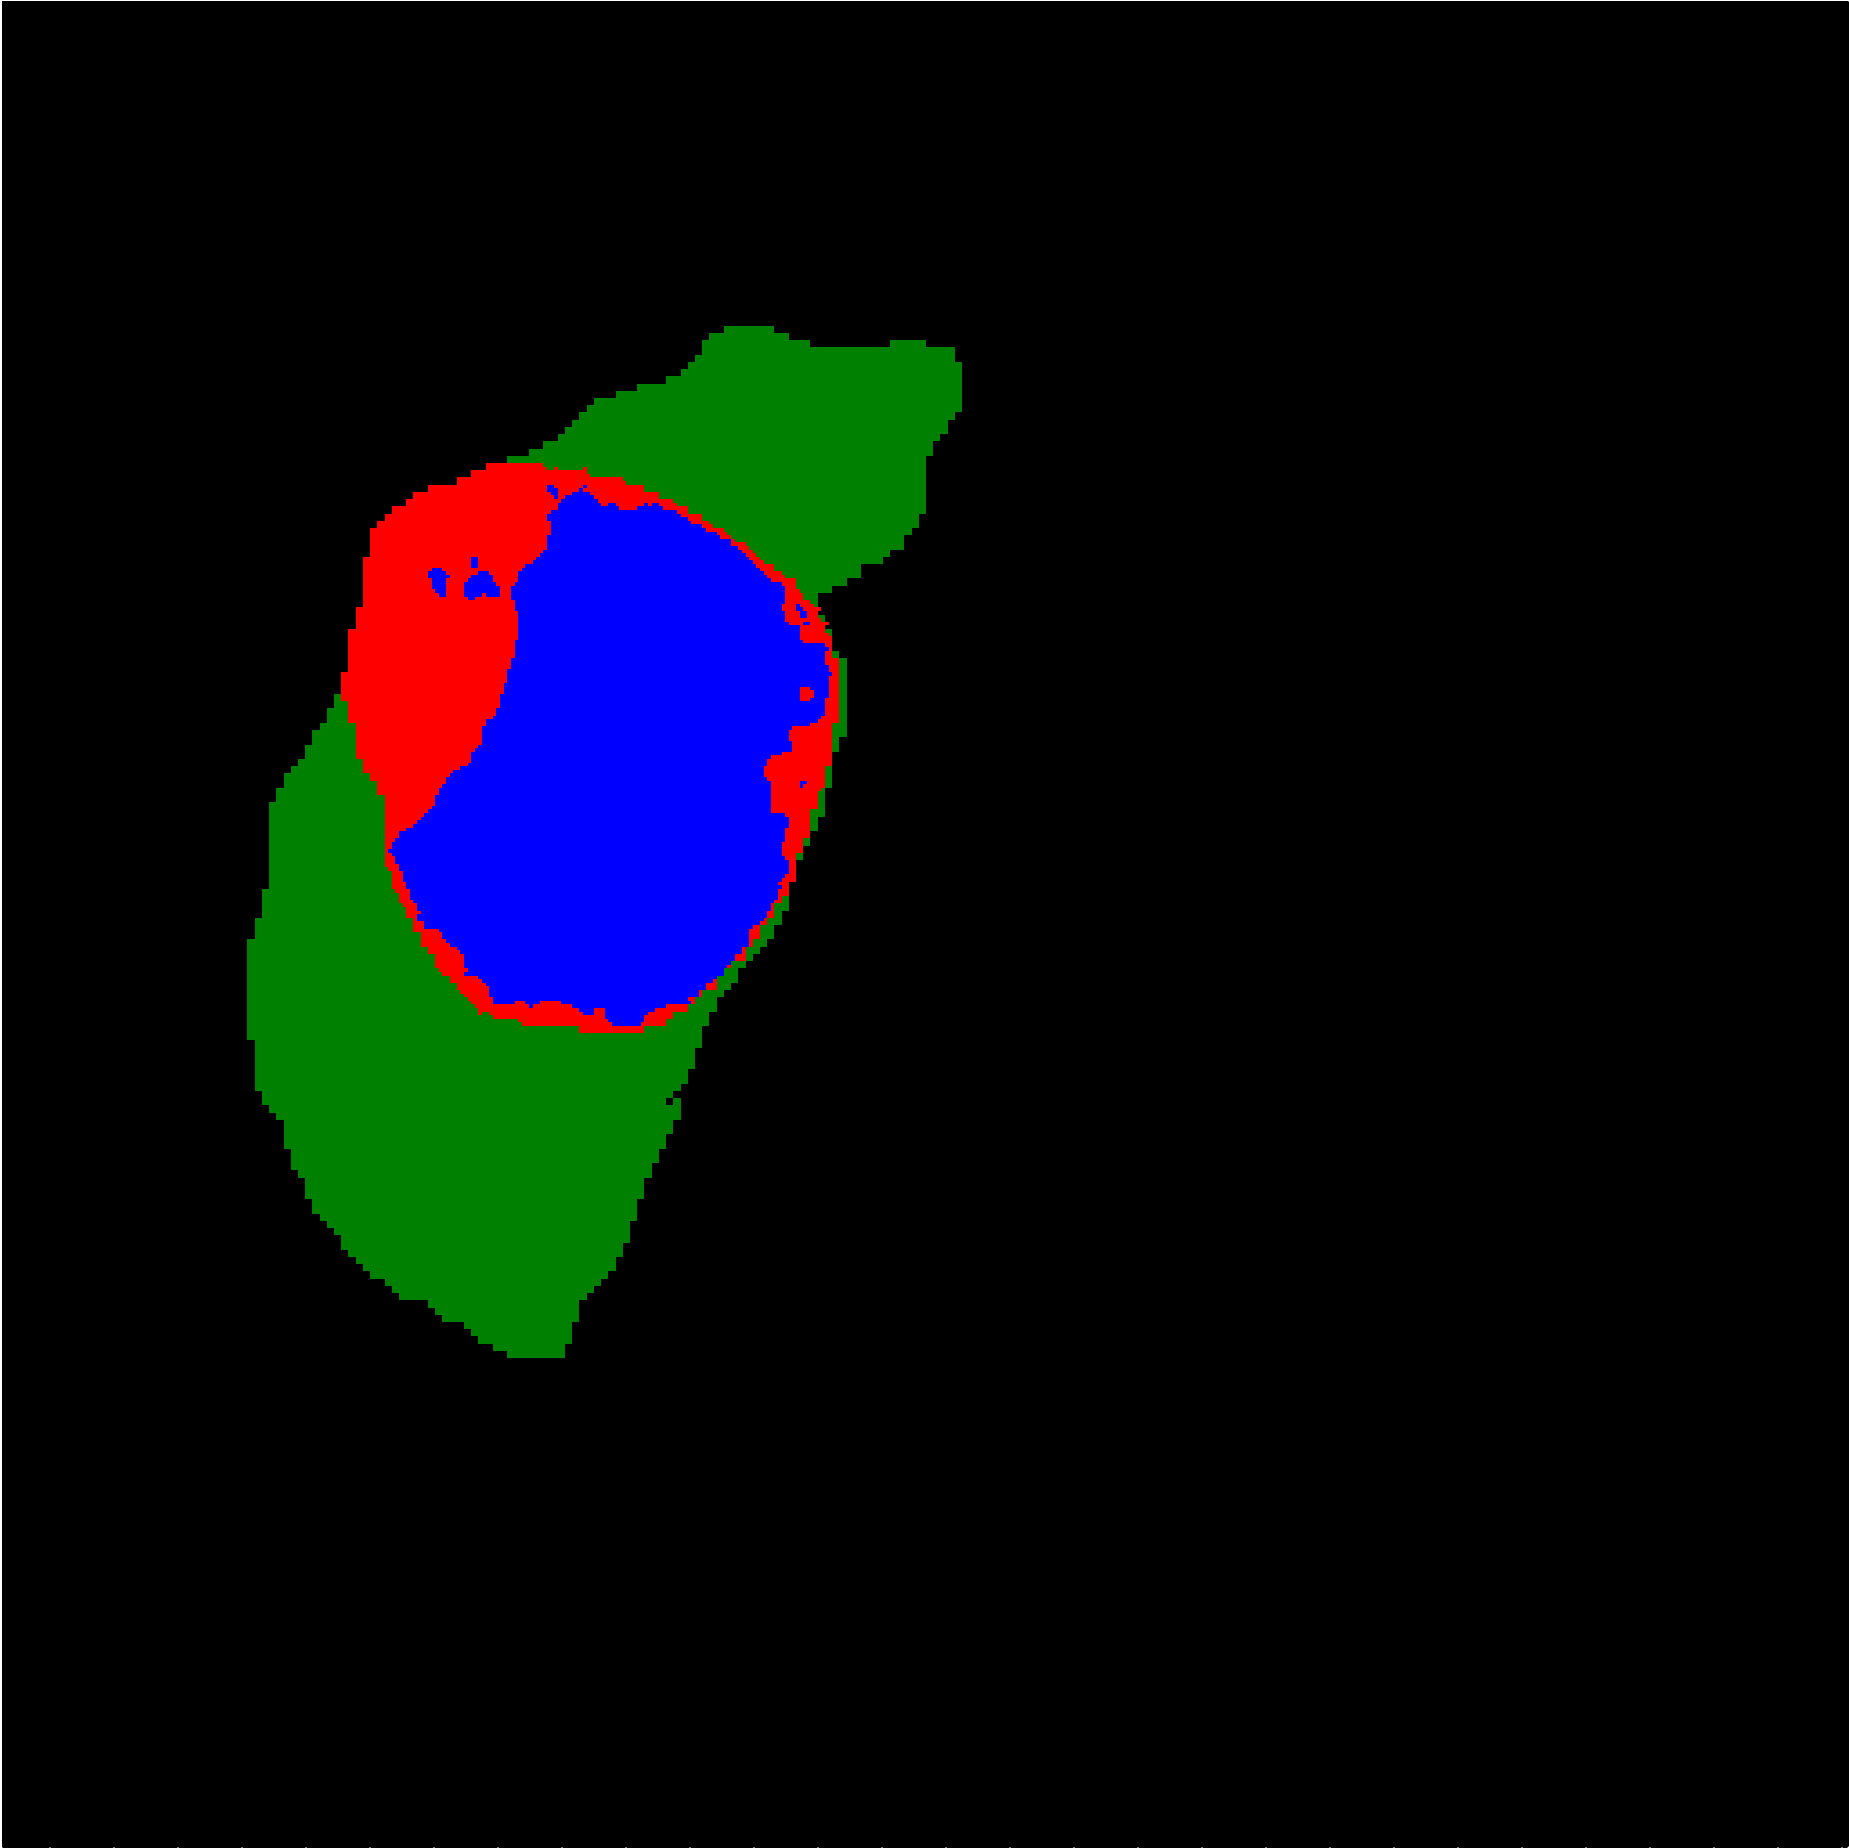
\includegraphics[width=\linewidth]{../SemanticSeg/images/1_7_FullAuto_new_resized}
\end{minipage} \hspace{-0.3cm}
\begin{minipage}{4cm}
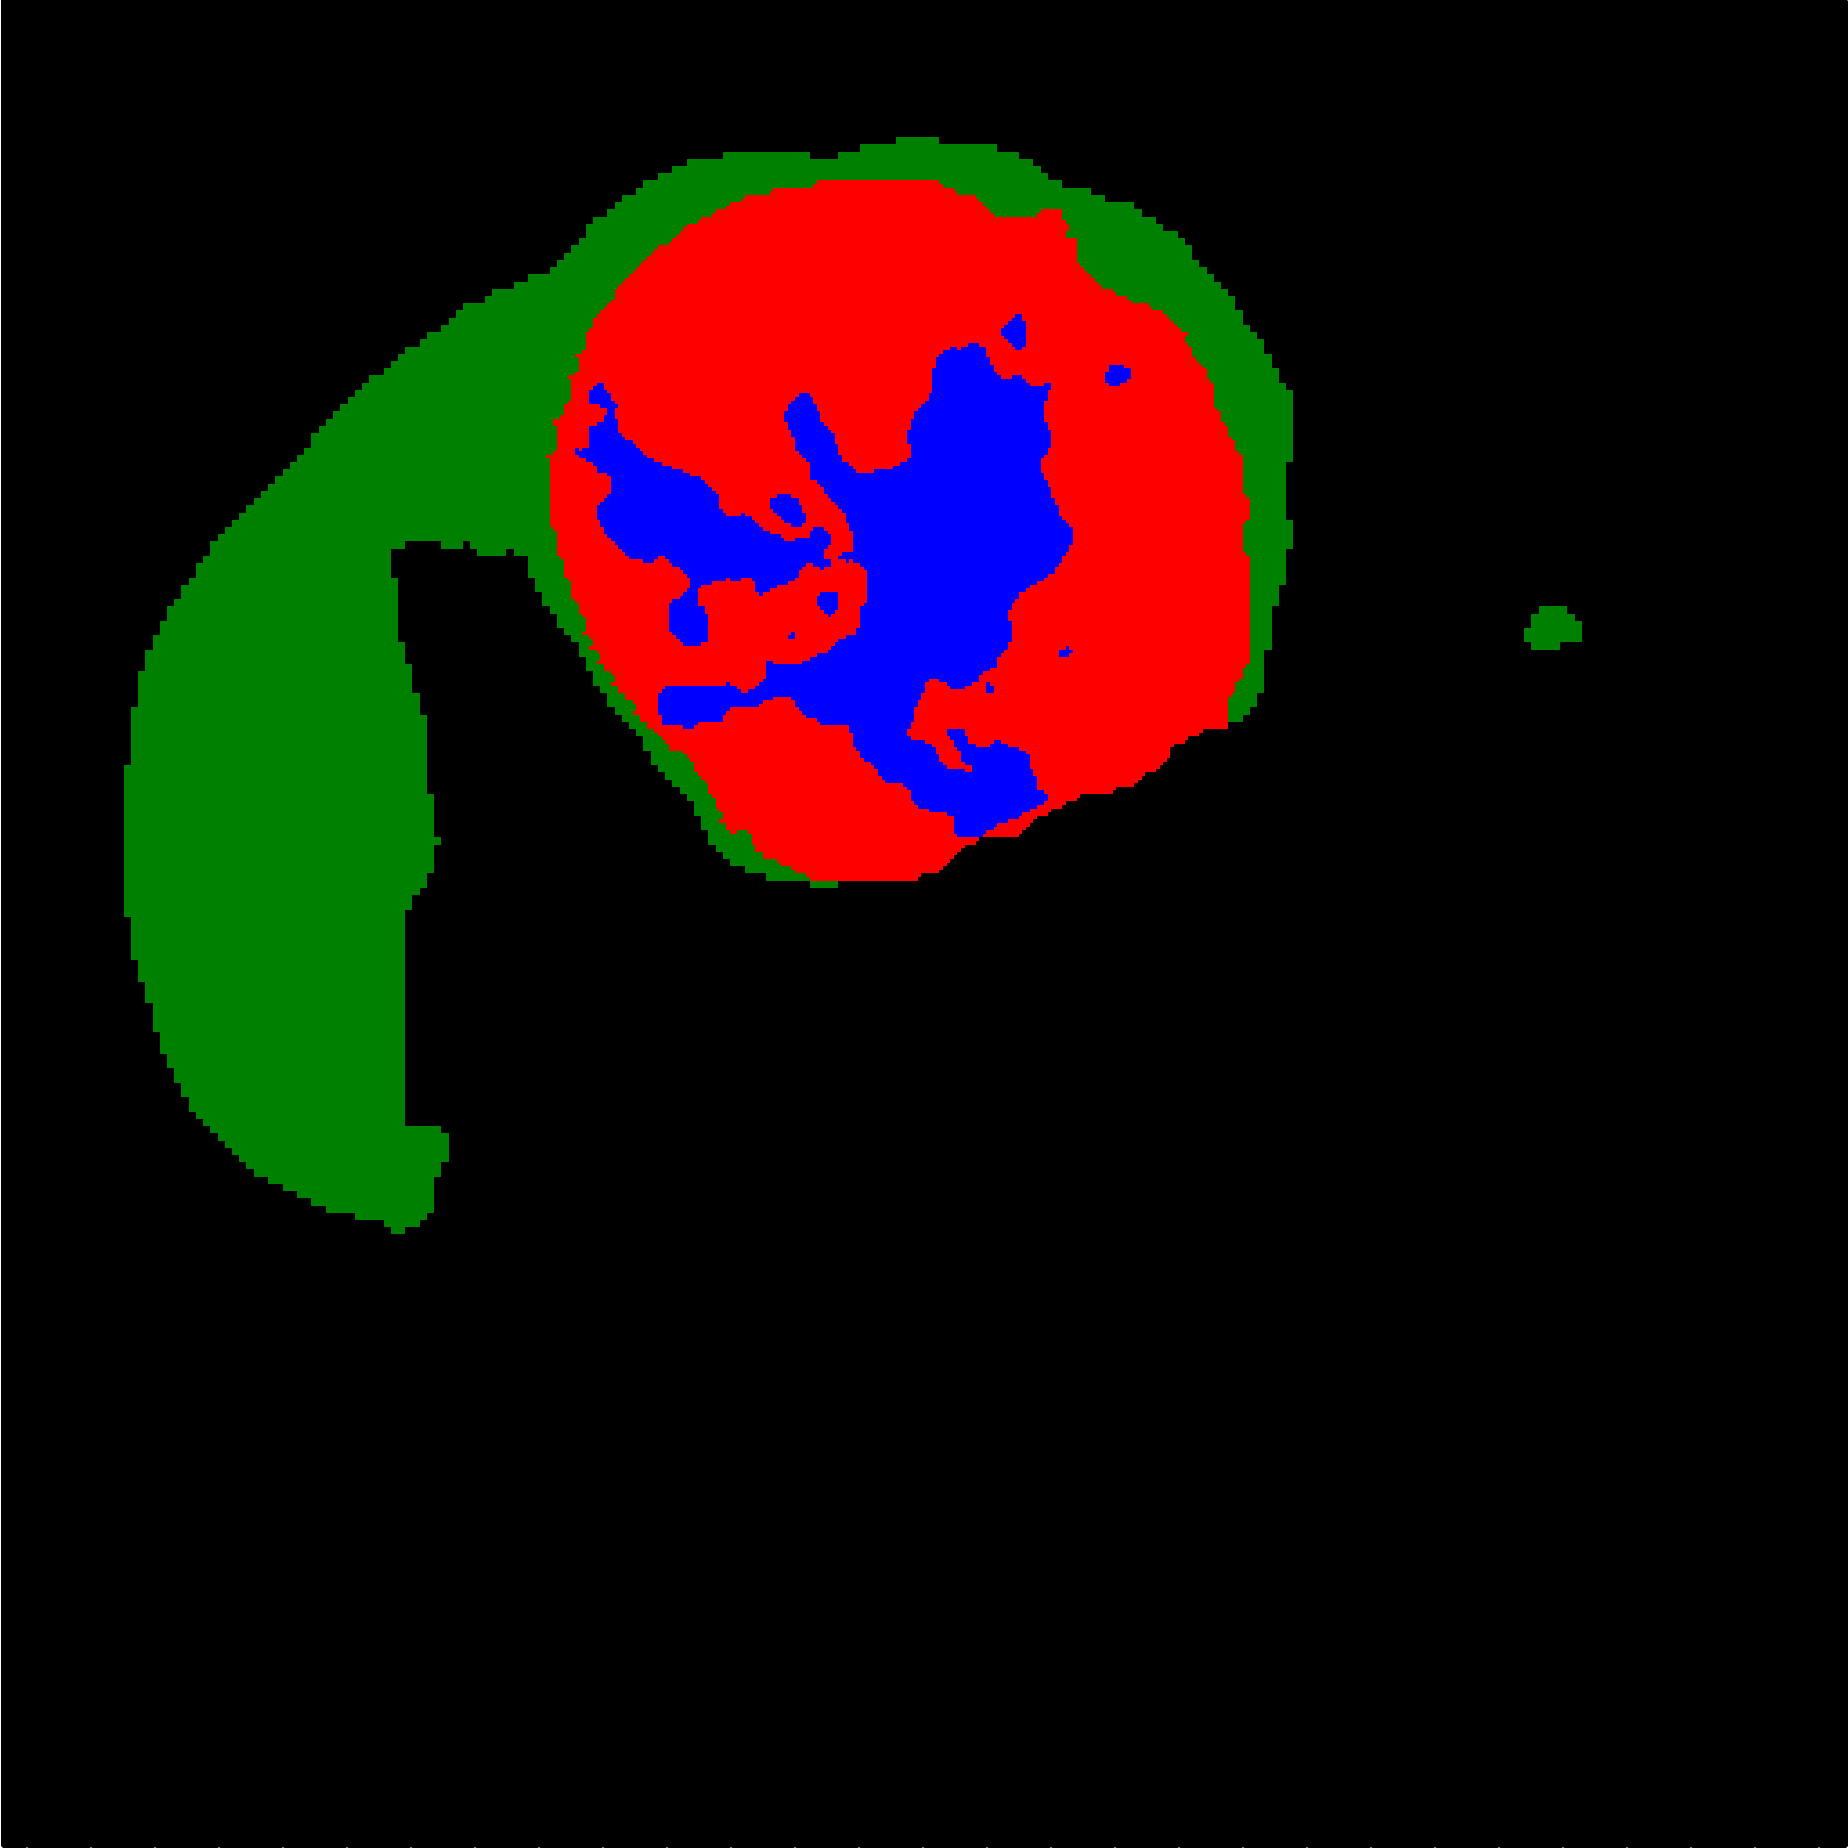
\includegraphics[width=\linewidth]{../SemanticSeg/images/2_3_FullAuto_resized}
\end{minipage} \hspace{-0.3cm}
\begin{minipage}{4cm}
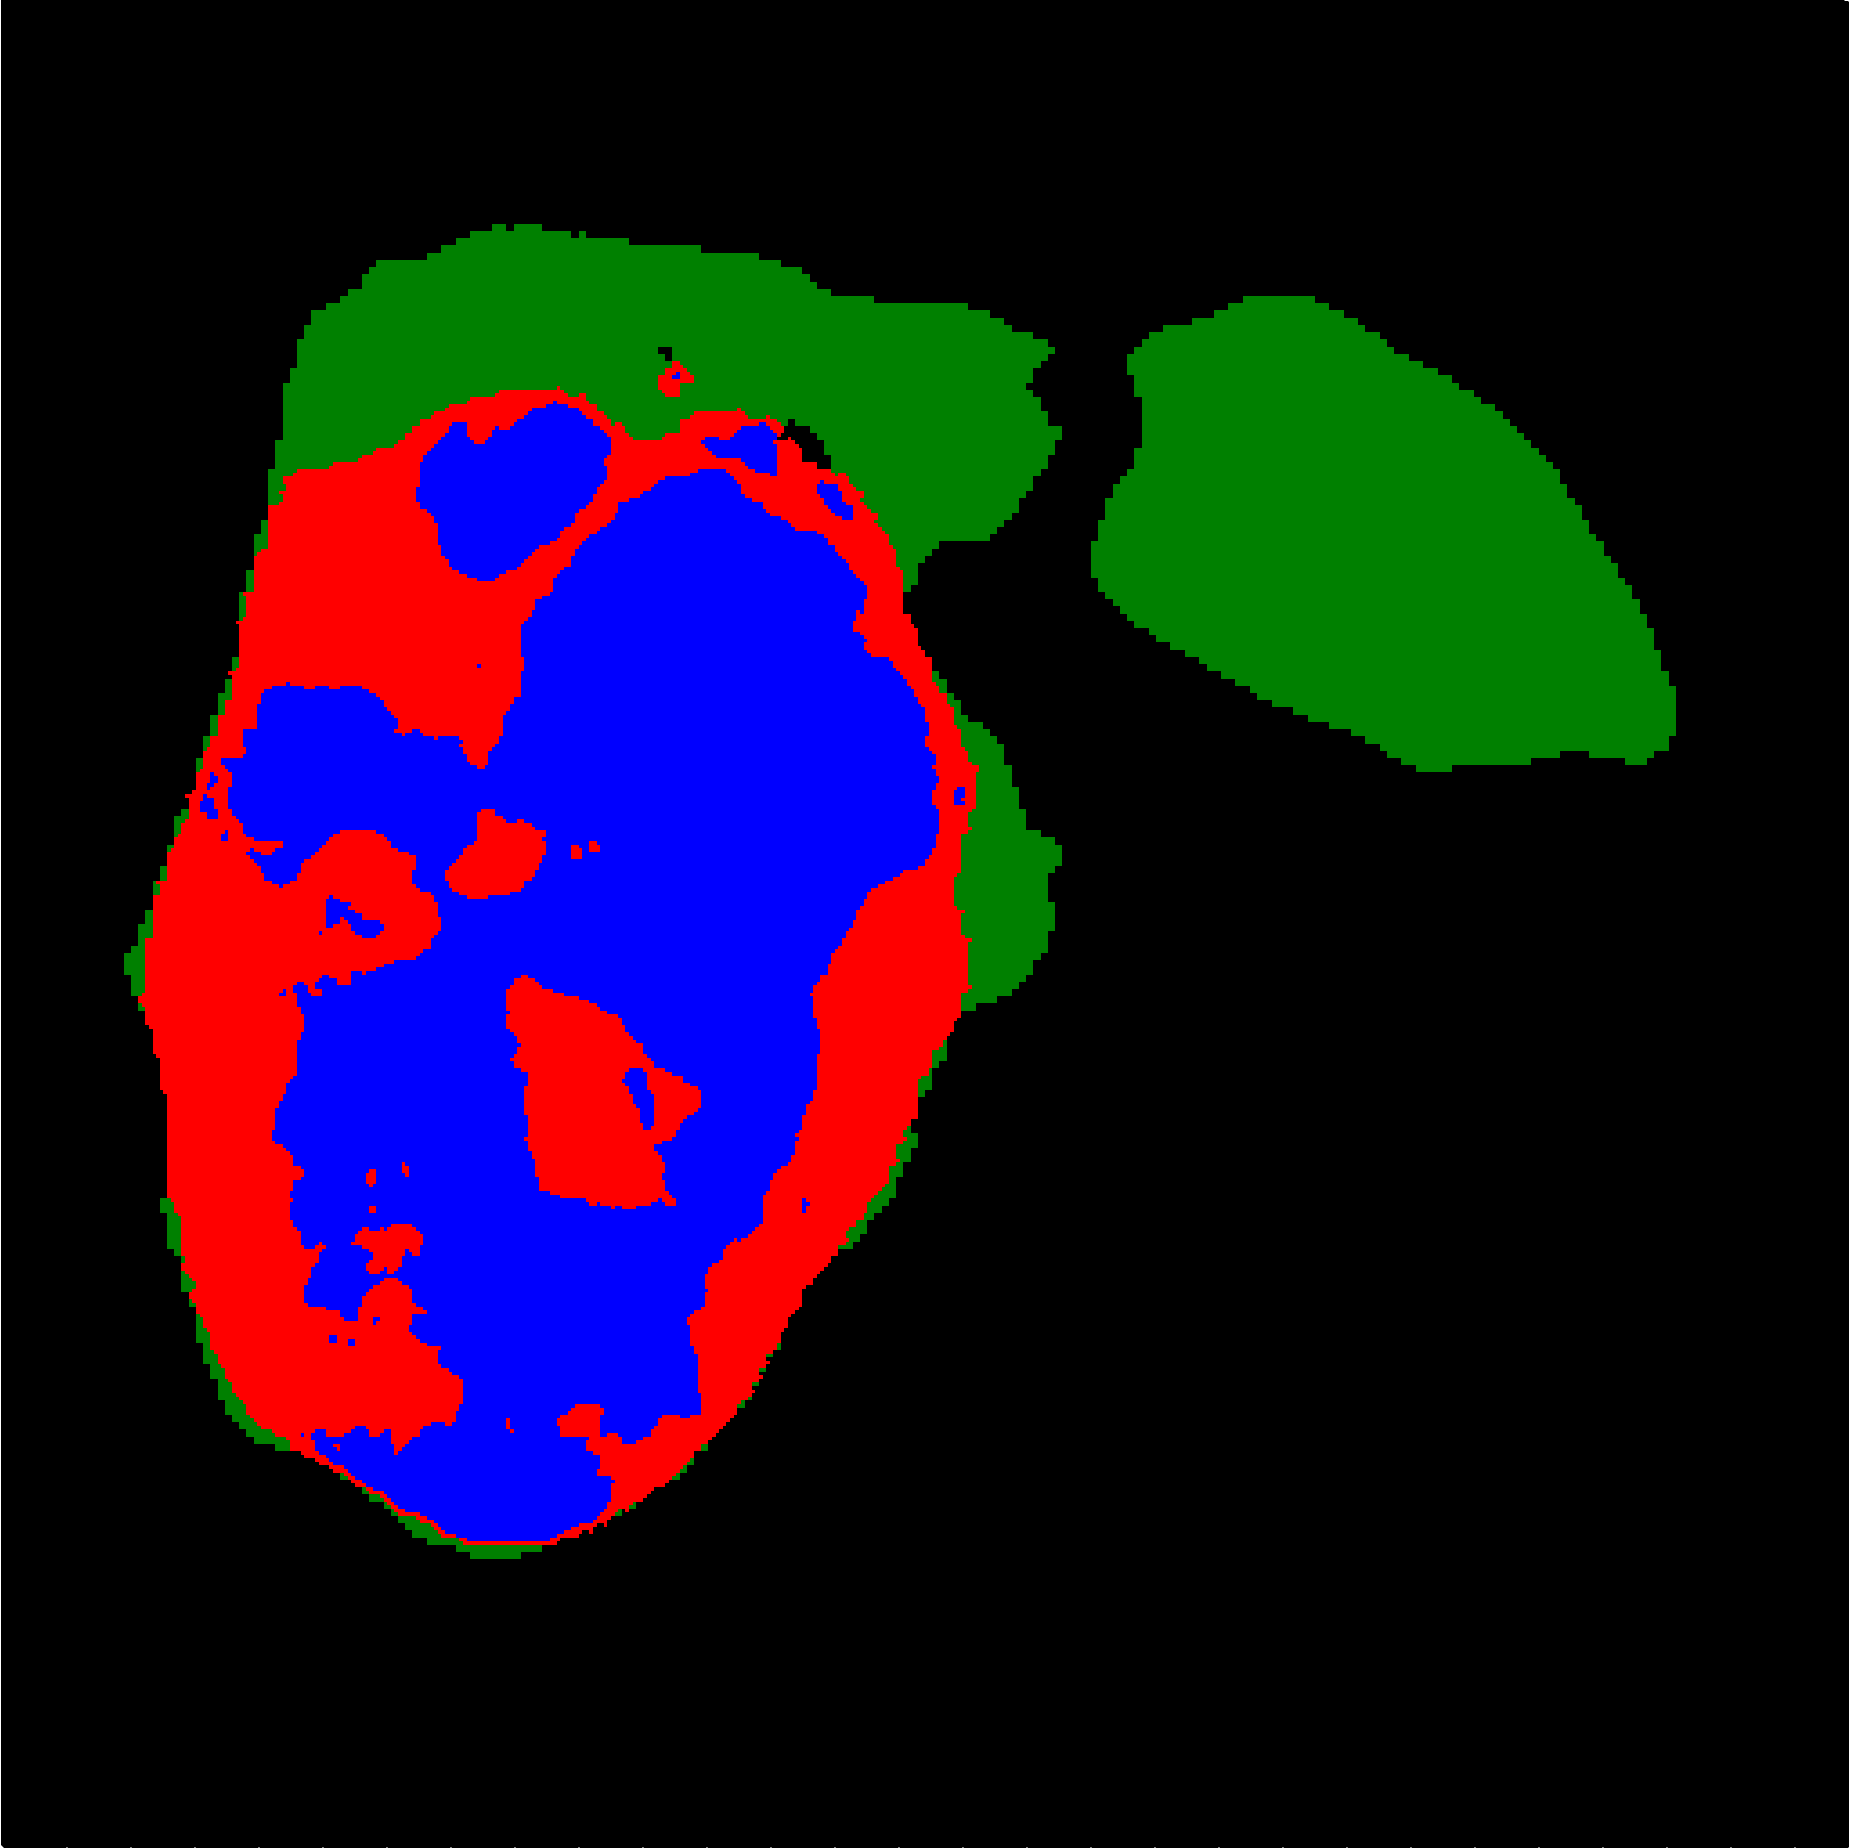
\includegraphics[width=\linewidth]{../SemanticSeg/images/5_4_FullAuto_resized}
\end{minipage} 
\caption{From top to bottom : Raw images, ground truth and results of the fully automatic segmentation of liver tissue}
\label{FullAutoSeg}
\end{figure}
\renewcommand{\baselinestretch}{1.75}
\renewcommand{\arraystretch}{5}


When comparing results obtained by the specialized networks, we proved
that the addition of the multiphase information provided better
segmentation results than when only single phase images are used.
Statistically significant improvement was obtained for the segmentation
of both the liver and the active part of the tumors.
We also investigated the performances of the single phase networks, and
noticed that the \ac{pv} phase was the one providing the best results,
where significant improvement was obtained for all the segmentation
tasks, except for the liver segmentation.
Regarding the internal liver tissues segmentation, the elementary
networks providing the best results were the \pplfont{DMP-Lesion} 
and \pplfont{DMP-Necrosis} ones. When combined in a cascaded way, 
they performed better than each one of the \pplfont{\{.\}-Full} architecture, 
with a statistically significant improvement
for the segmentation of the active part of the lesions, meaning that 
combining several specialized networks together is more efficient 
than training a single network addressing all tasks simultaneously.\\
With the same experimental conditions, our solution provided a better
accuracy for the segmentation of the lesions, and for both their active
and the necrotic parts, than the one obtained using a semi-automatic
technique with expert interaction \cite{Ouhmich2019,Conze2017}. We also
obtained equivalent results than those from a similar study considering
MR images as input \cite{Zhang2018}.\\
We concluded that the combination of multiphase registered images used in a 
cascaded architecture allows us to automatically perform the semantic segmentation of liver tissues.


\subsubsection{Semantic segmentation applied to weakly annotated datasets}

We proved that semantic segmentation of liver tissues can be
performed using \ac{dl} through robust CV training on both \textbf{\lmttfont{3DIrcad-dB}} and
\textbf{\lmttfont{TheraHCC-dB}}.
We also demonstrated that both a cascaded architecture and the use of
multiphase information allows a better segmentation accuracy than using
single phase images only.
We will now extend our work to prove the ability of semantic segmentation architecture to provide missing annotations into weakly annotated datasets such as \textbf{\lmttfont{TCIA-dB}}.\\
\textbf{\lmttfont{TCIA-dB}} originally only
contained raw images without annotations, so an expert performed the
delineations for both the tumor and the necrosis areas on \ac{pv} images only. \\
To achieve a multiphasic semantic segmentation of the liver tissues we
have to ensure that both the liver and its internal structures such as
the potential tumors are located at the same spatial position between
the different \ac{cect} volumes.


\paragraph{Registration}\label{registration}

\begin{figure}[th!]
\centering
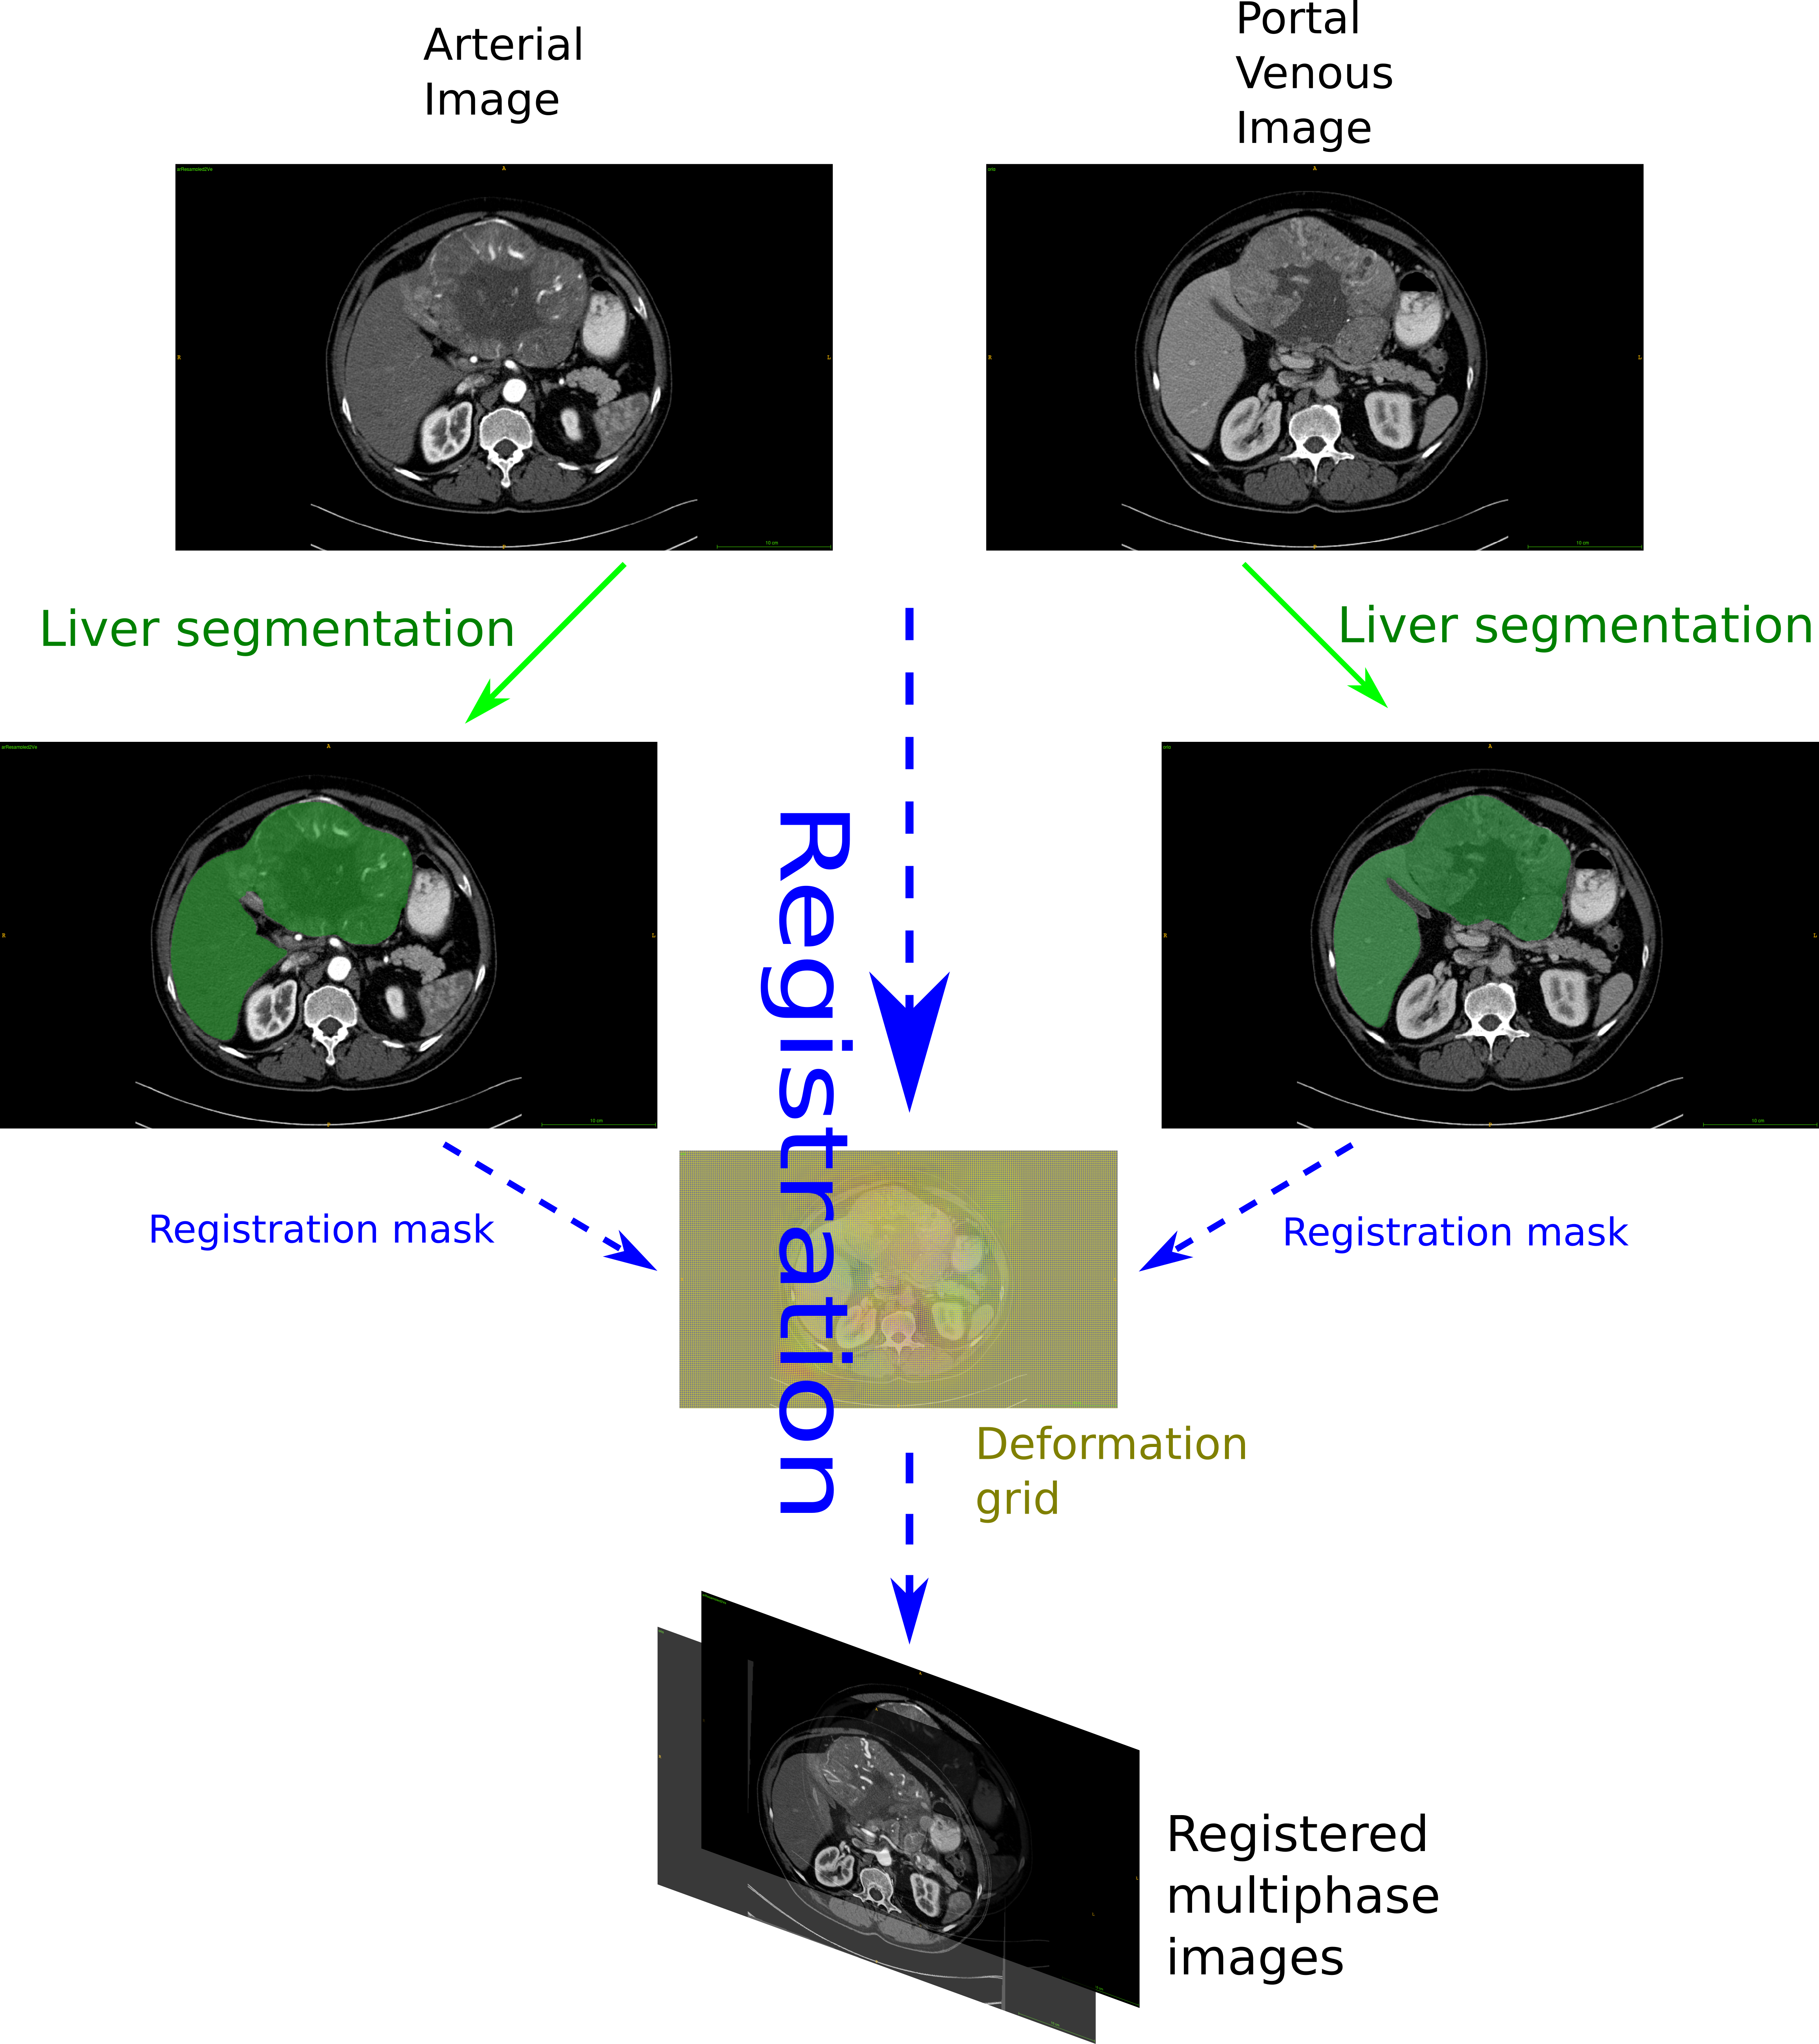
\includegraphics[width=0.7\linewidth]{../HistologicalGradePrediction/images/RegistrationTCIA_pipeline_vertical2}
\caption{Illustration of the registration pipeline applied to the images of \textbf{\lmttfont{TCIA-dB}}. The first green arrows correspond to the liver segmentation using a network trained on the \textbf{\lmttfont{LITS-dB}}. Dashed blue arrows correspond to the ANTs registration pipeline, where a dilated version of the predicted liver annotations maps are used as registration masks. The ANTs algorithm implements 3 transformations: a rigid, an affine, and a diffeomorphic Syn transformation that computes a deformation grid \cite{Avants2008}. The 3 steps of the ANTs algorithm allows us to obtain registered multiphase images.}
\label{fig:RegistrationTCIA_pipeline_vertical2}
\end{figure}


One way to perform a registration is to implement a series of
transformations (rigid or non-rigid) that will match a moving volume to
a target one. Each step of the registration is controlled by a
similarity loss.
When dealing with \ac{ct} volumes the available losses controlling the
different steps of the registration pipeline can be affected by areas of
the body with a high gradient such as the bones for example. When
registering two \ac{ct} volumes, one can either directly use both the entire
volumes or constraints the registration to a specific area (aka mask).
The liver being a soft organ, it easily moves with the respiratory
motions, in order to reduce the effect of the neighboring parts of the
abdomen, we have decided to restrict the computation of the similarity
metrics to the dilated liver mask area so that the registration
algorithm mainly focus on the gradient present along its borders.

Consequently, the first step for the \textbf{\lmttfont{TCIA-dB}} registration is to perform a
liver semantic segmentation (green arrows in the figure \ref{fig:RegistrationTCIA_pipeline_vertical2}).

\paragraph{Automatic liver segmentation}\label{tcia-db-unsupervised-liver-segmentation}

In the available datasets (as presented in the table \ref{xp_datasets}), only \textbf{\lmttfont{TheraHCC-dB}} and
\lmttfont{LITS-dB} contained expert liver delineation.

\lmttfont{TheraHCC-dB} contains annotations only on sparse slices across the liver,
whereas \textbf{\lmttfont{LITS-dB}} contains full 3D pixel-wise liver annotation but it only
contains monophase images, without any information regarding the
acquisition phase (\ac{ar}, \ac{pv} and potentially DELAY volumes are mixed in the dataset).
Our experiments however showed that a liver segmentation network trained
on sufficiently enough cases is able to perform the semantic
segmentation of both \ac{ar} and \ac{pv} raw images independently.
We trained our network called \pplfont{\ac{cect}-Liver} on the 131 volumes of the
\lmttfont{LITS-dB} using the same hyperparameters as the ones detailed
previously. When testing the \pplfont{\ac{cect}-Liver} network on \textbf{\lmttfont{TheraHCC-dB}} we
obtained a mean slice-wise \ac{dsc} of $ 90.4 \pm 17.5 $ on the \ac{pv} images and
$ 86.9 \pm 19.1 $ on the \ac{ar} images. These results, close to those obtained
in our previous work using a CV approach \cite{Ouhmich2019}, proved that \pplfont{\ac{cect}-Liver} can
perform liver segmentation on both \ac{ar} and \ac{pv} unseen images.

The \pplfont{CECT-Liver} network was also able to segment unseen volumes of the
\textbf{\lmttfont{TCIA-dB}} in both \ac{ar} and \ac{pv} phases even when the liver presents a big
lesion, as we can see in the figure \ref{fig:LiverPredTciaDb}.

\begin{figure}[ht!]
\centering
\begin{minipage}{0.45\linewidth}
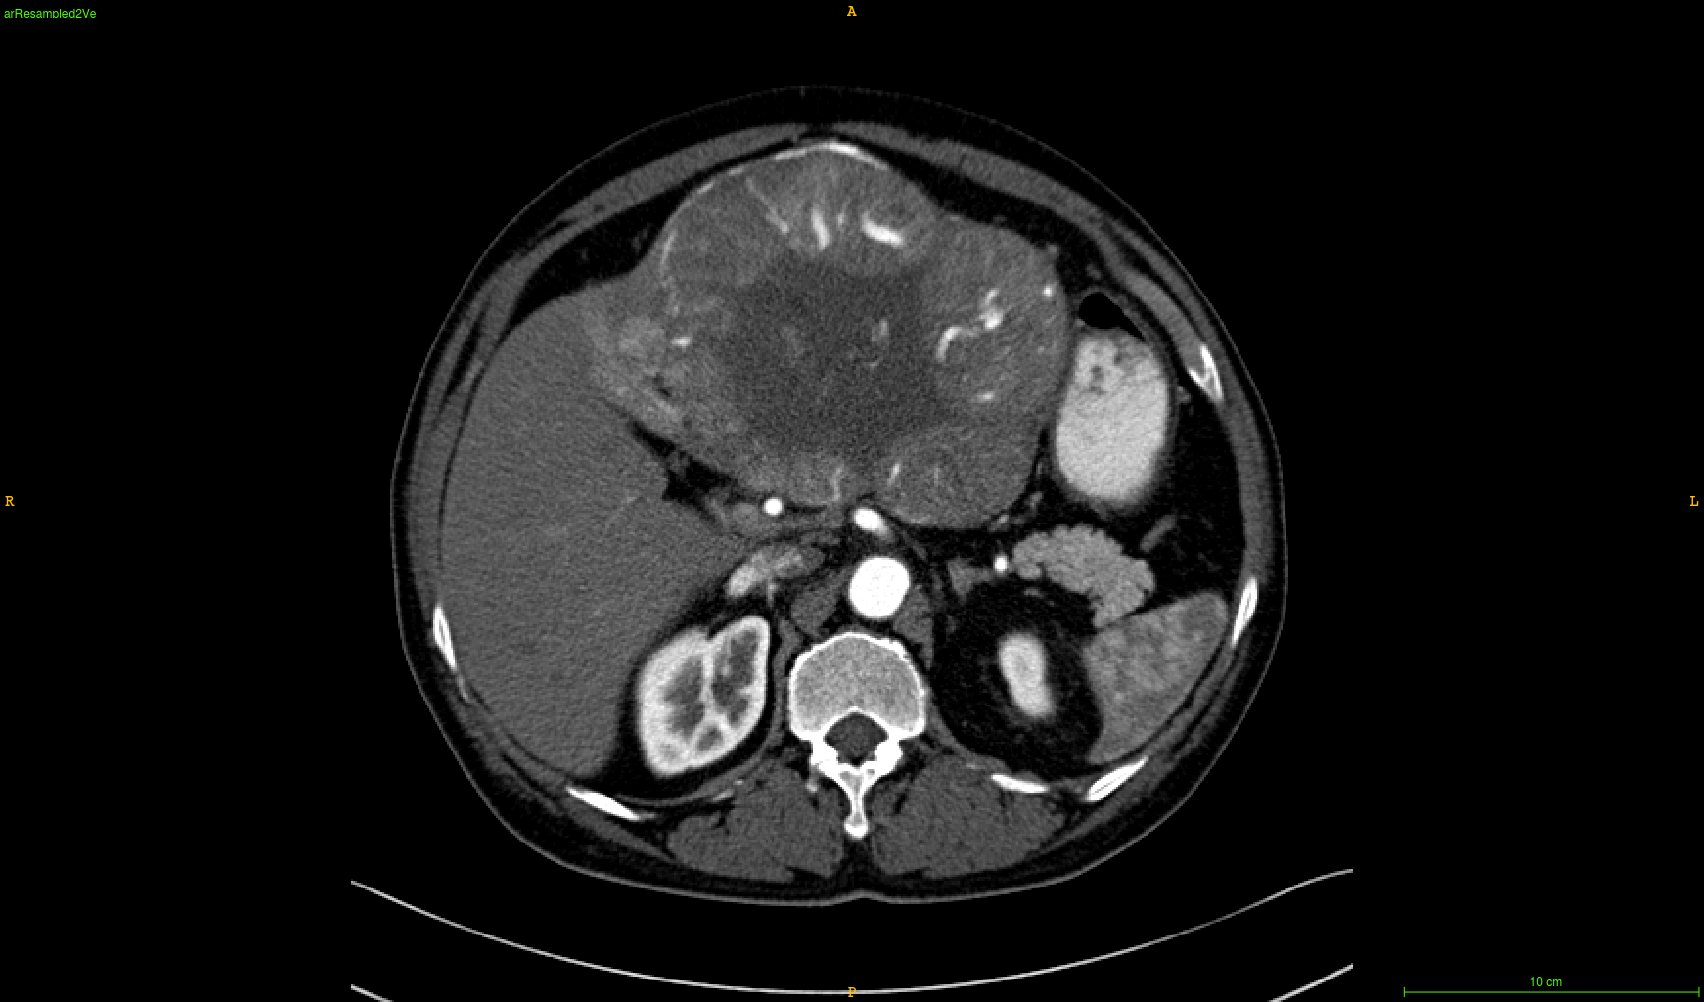
\includegraphics[width=0.9\linewidth]{../HistologicalGradePrediction/images/TCIA_CECTLiver_prediction_TCGA-DD-A11A_slice42_AR_raw}
\end{minipage}
\hspace{0.3cm}
\begin{minipage}{0.45\linewidth}
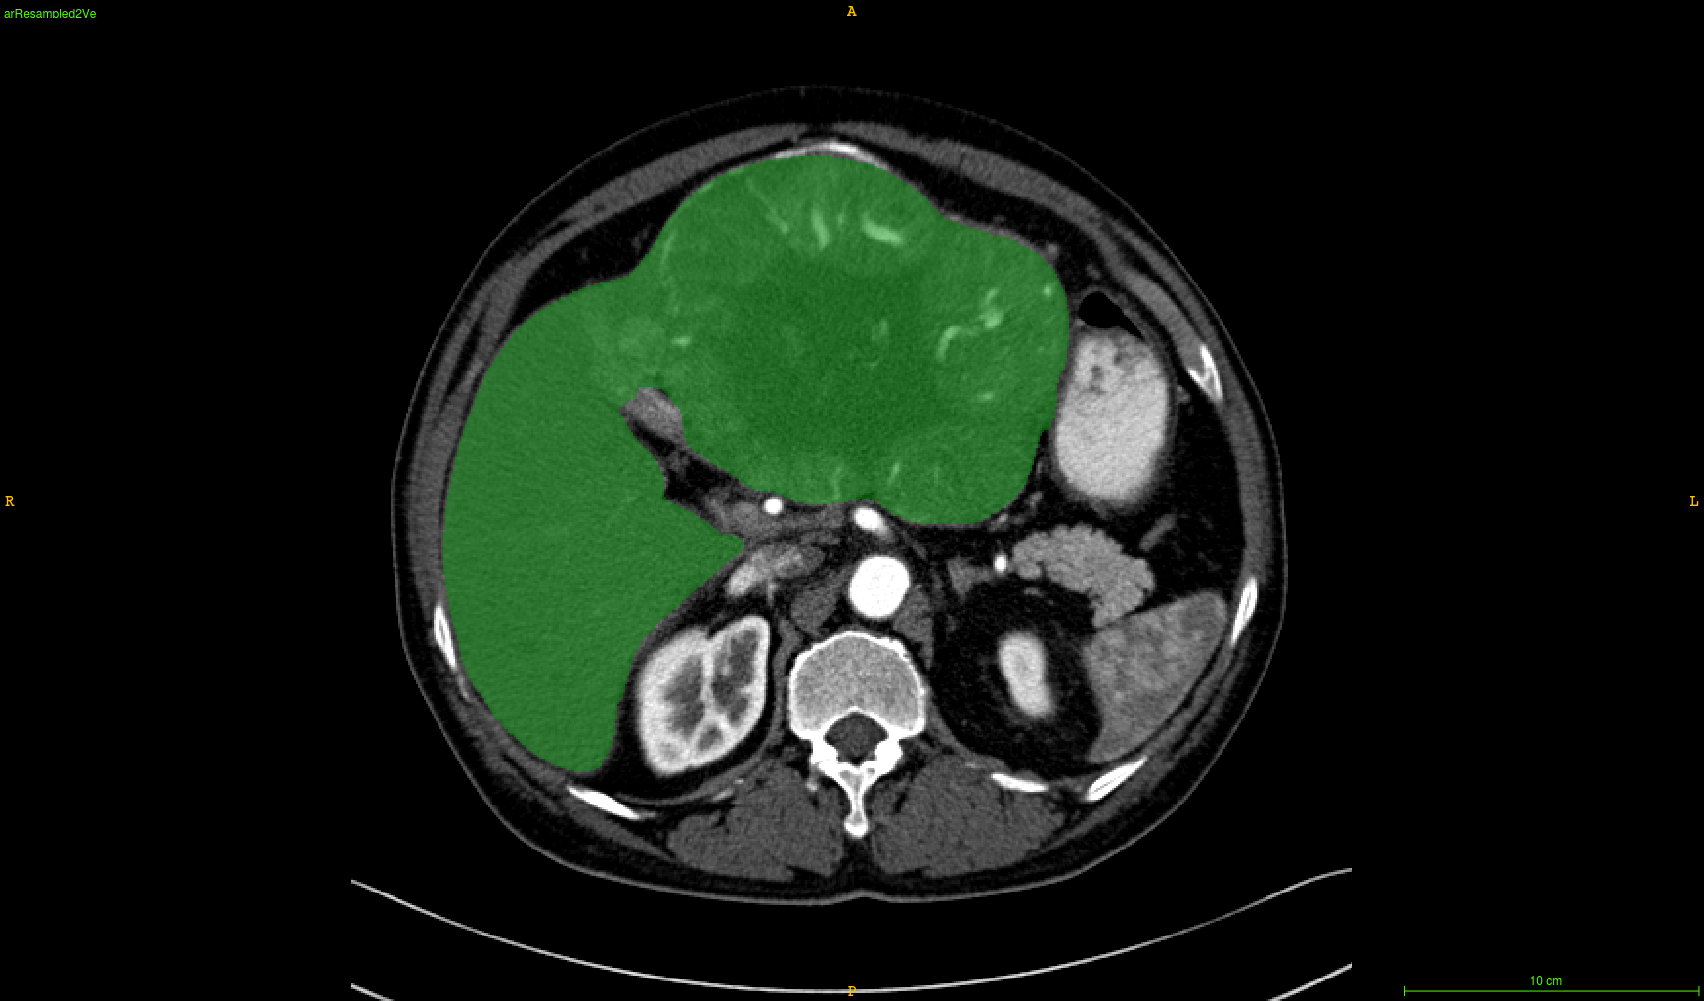
\includegraphics[width=0.9\linewidth]{../HistologicalGradePrediction/images/TCIA_CECTLiver_prediction_TCGA-DD-A11A_slice42_AR_green_liver}
\end{minipage}

\vspace{0.8cm}
\begin{minipage}{0.45\linewidth}
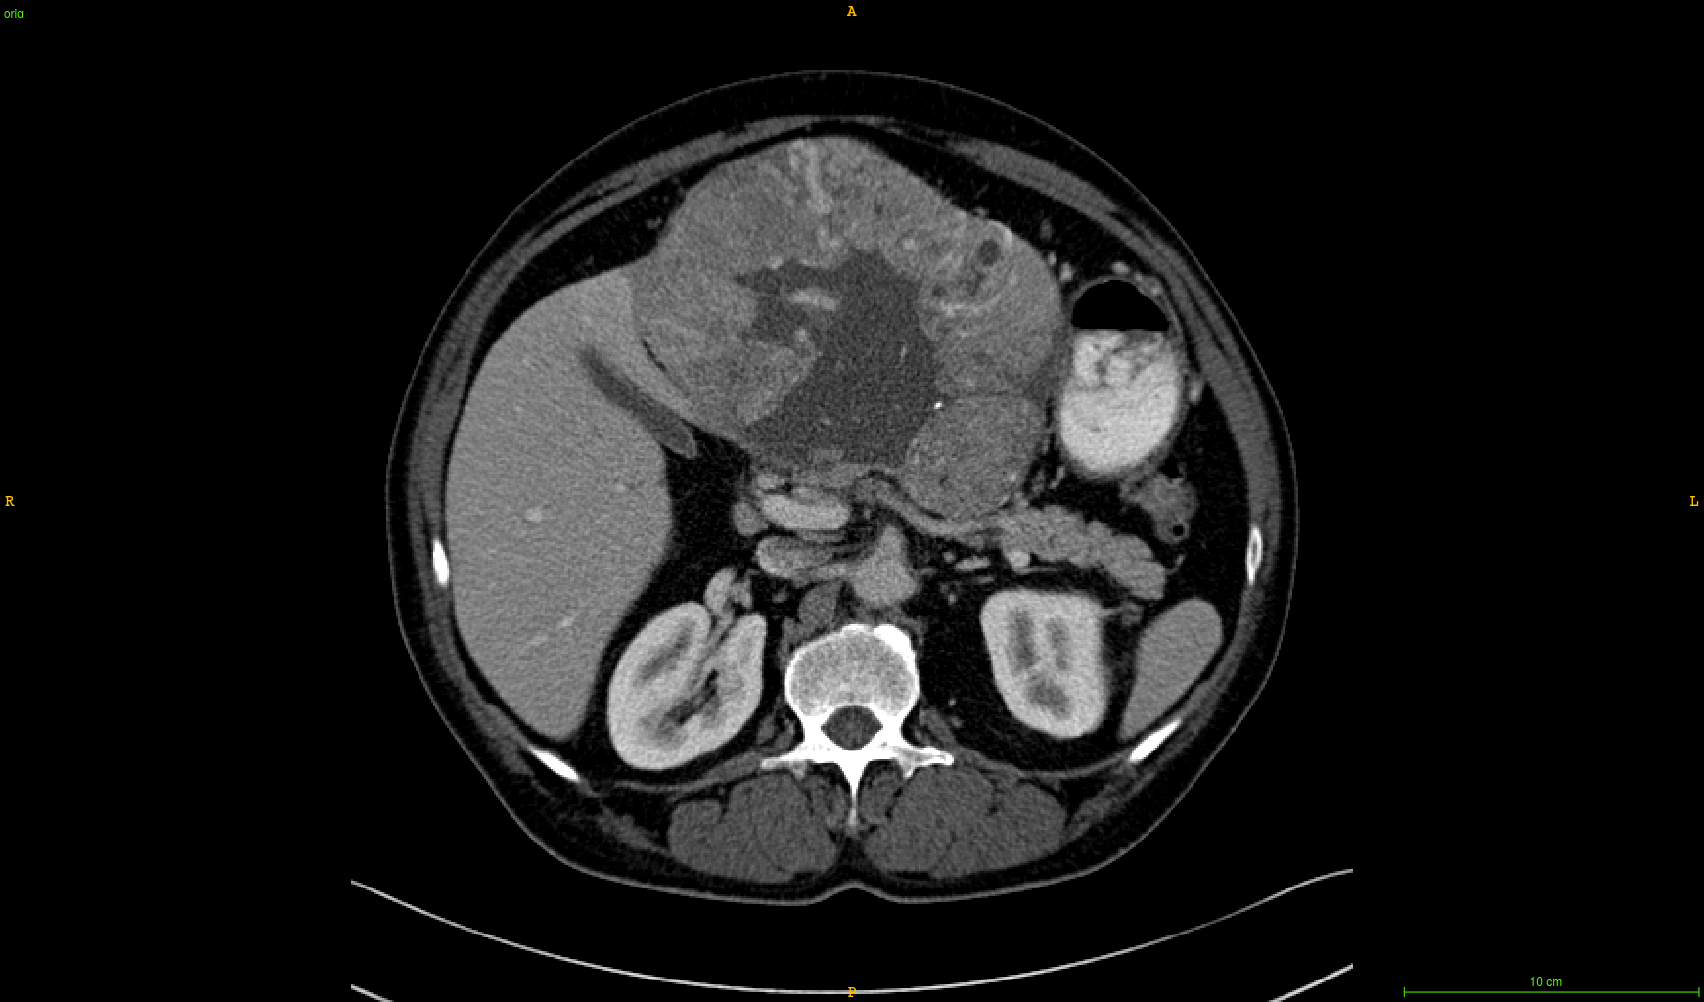
\includegraphics[width=0.9\linewidth]{../HistologicalGradePrediction/images/TCIA_CECTLiver_prediction_TCGA-DD-A11A_slice42_raw}
\end{minipage}
\hspace{0.3cm}
\begin{minipage}{0.45\linewidth}
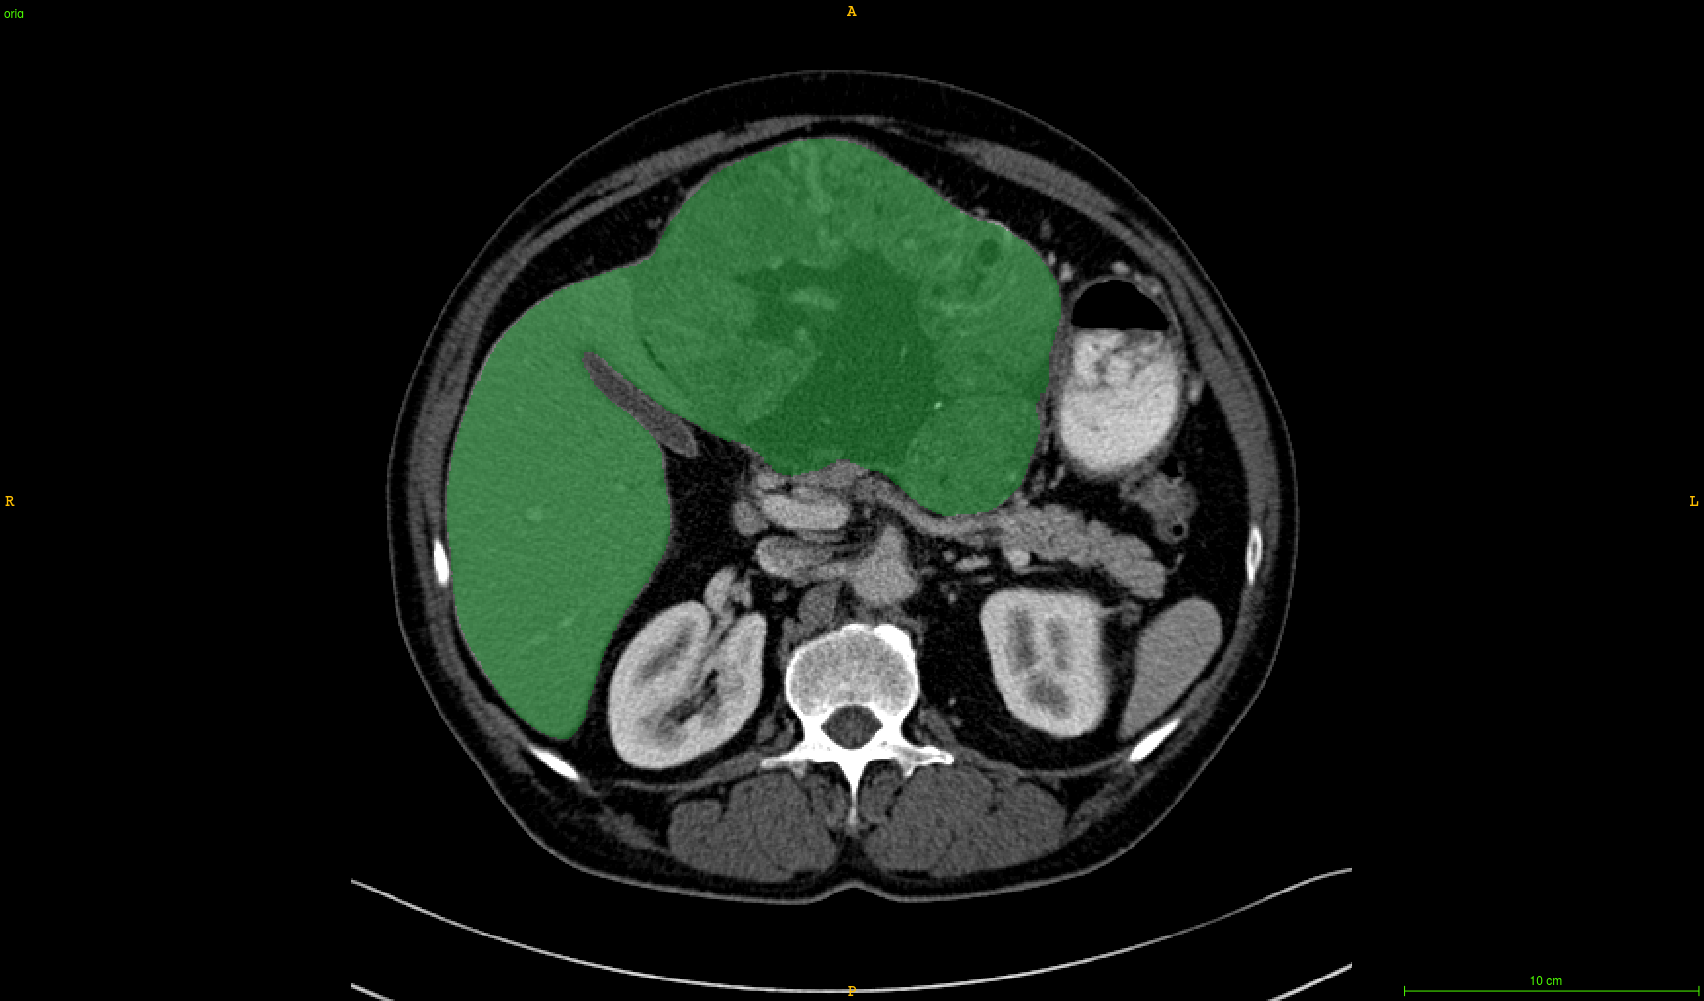
\includegraphics[width=0.9\linewidth]{../HistologicalGradePrediction/images/TCIA_CECTLiver_prediction_TCGA-DD-A11A_slice42_greenLiver}
\end{minipage}
\caption{Example of liver segmentation using the \pplfont{\ac{cect}-Liver} network on \lmttfont{TCIA-dB}
patients (Top row \ac{ar} images, bottom row: \ac{pv} images, left:
Raw images, right : liver segmentation as overlay).}
\label{fig:LiverPredTciaDb}
\end{figure}



Once a robust liver segmentation was obtained, we implemented our
registration pipeline.

We have decided to implement the registration pipeline using ANTs \cite{avants2009advanced}, since it has already been used for liver
CT scans registration \cite{Zhao2019,Zhao2020}.

\paragraph{ANTs registration}\label{tcia-db-ants-registration}

The classical ANTs registration pipeline is made of 3 steps. The first
two steps consist of linear transformations, where a rigid
transformation is first applied, followed by an affine transformation.
The last one is generally non-linear. In our pipeline,
we used a Syn (\emph{Standard Symmetric normalisation}) transformation, which
processes a gradient field, determining how each point of the space will
shift \cite{Avants2008}.

The MI (Mutual Information) was used as loss function for the first two
steps because it has the advantage of computing the similarity at a
large scale. Linear rigid and affine transformations tend to roughly bring both volumes
in the same space so we decided not to use a finer similarity metric. For the Syn
transformation, we used the CC (Cross Correlation) as loss function. The CC
has the advantage of looking precisely in a region around each voxel
when computing the similarity between the two volumes.

During the registration process, the liver segmentation was used as
registration mask, and we decided to set the \ac{pv} volume as target (fixed)
volume since it usually presents the finer voxel resolution when
compared to \ac{ar} (or DELAY) volume, and since it contains the original
expert annotations.

\begin{figure}
\fbox{
\parbox{\textwidth}{
\begin{enumerate}
\item We initially resampled the \ac{ar} volume so it has the same resolution as the corresponding \ac{pv} volume.
\item We performed the liver segmentation using \pplfont{\ac{cect}-Liver} on both the \ac{pv} and the resampled \ac{ar} volumes in a slice-wise manner with a classical post-processing consisting in applying a binary opening operation to the mask and conserving the big connected component (see green arrows in the figure \ref{fig:RegistrationTCIA_pipeline_vertical2}). We obtained a liver mask for both the \ac{pv} and the resampled \ac{ar} volumes.
\item We applied the registration using both dilated version of the two masks obtained at the end of the second step as registration masks (as depicted by the dashed blue arrows in the figure \ref{fig:RegistrationTCIA_pipeline_vertical2}) (we dilated the liver mask with a SSE of 5cm when setting the registration mask in order to counter any error in the segmentation process, and to always have both the liver and its border included in the registration mask)
\end{enumerate}}}
\captionof{table}{Registration pipeline} \label{regisPipeline}
\end{figure}

The registration allows us to obtain both a new registered arterial volume, a transformation matrix and a deformation field volume. In the axial plane, the obtained deformation fields tend to present high deformation at both the top and the bottom of the liver (which can be explained anatomically since they are surrounded by the air and will be more subject to deformation than central areas of the liver) whereas central areas of the liver present high deformation close to the border. Examples of obtained deformation fields at the end of the registration pipeline are depicted in the figure \ref{fig:deformationGridExamples}.

\begin{figure}
\centering
\begin{minipage}{0.7\linewidth}
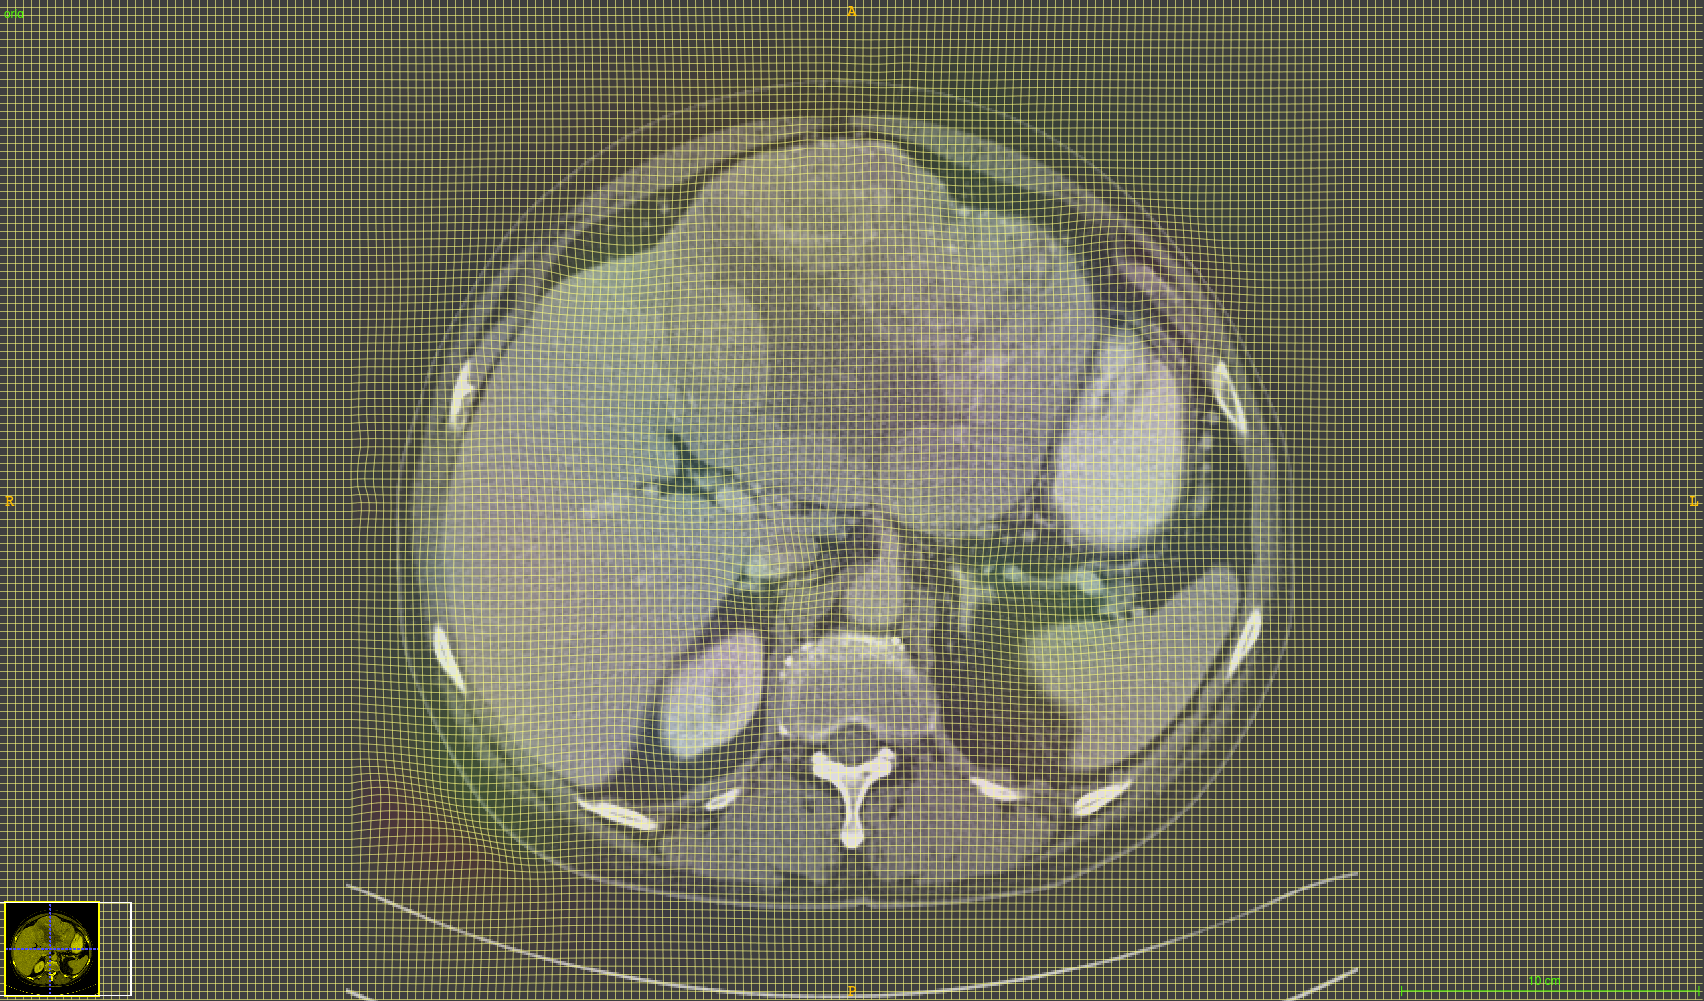
\includegraphics[width=\linewidth]{../HistologicalGradePrediction/images/TCIA_TCGA-DD-A11A_deformation_grid_slice49}
\end{minipage}

\vspace{0.8cm}
\begin{minipage}{0.7\linewidth}
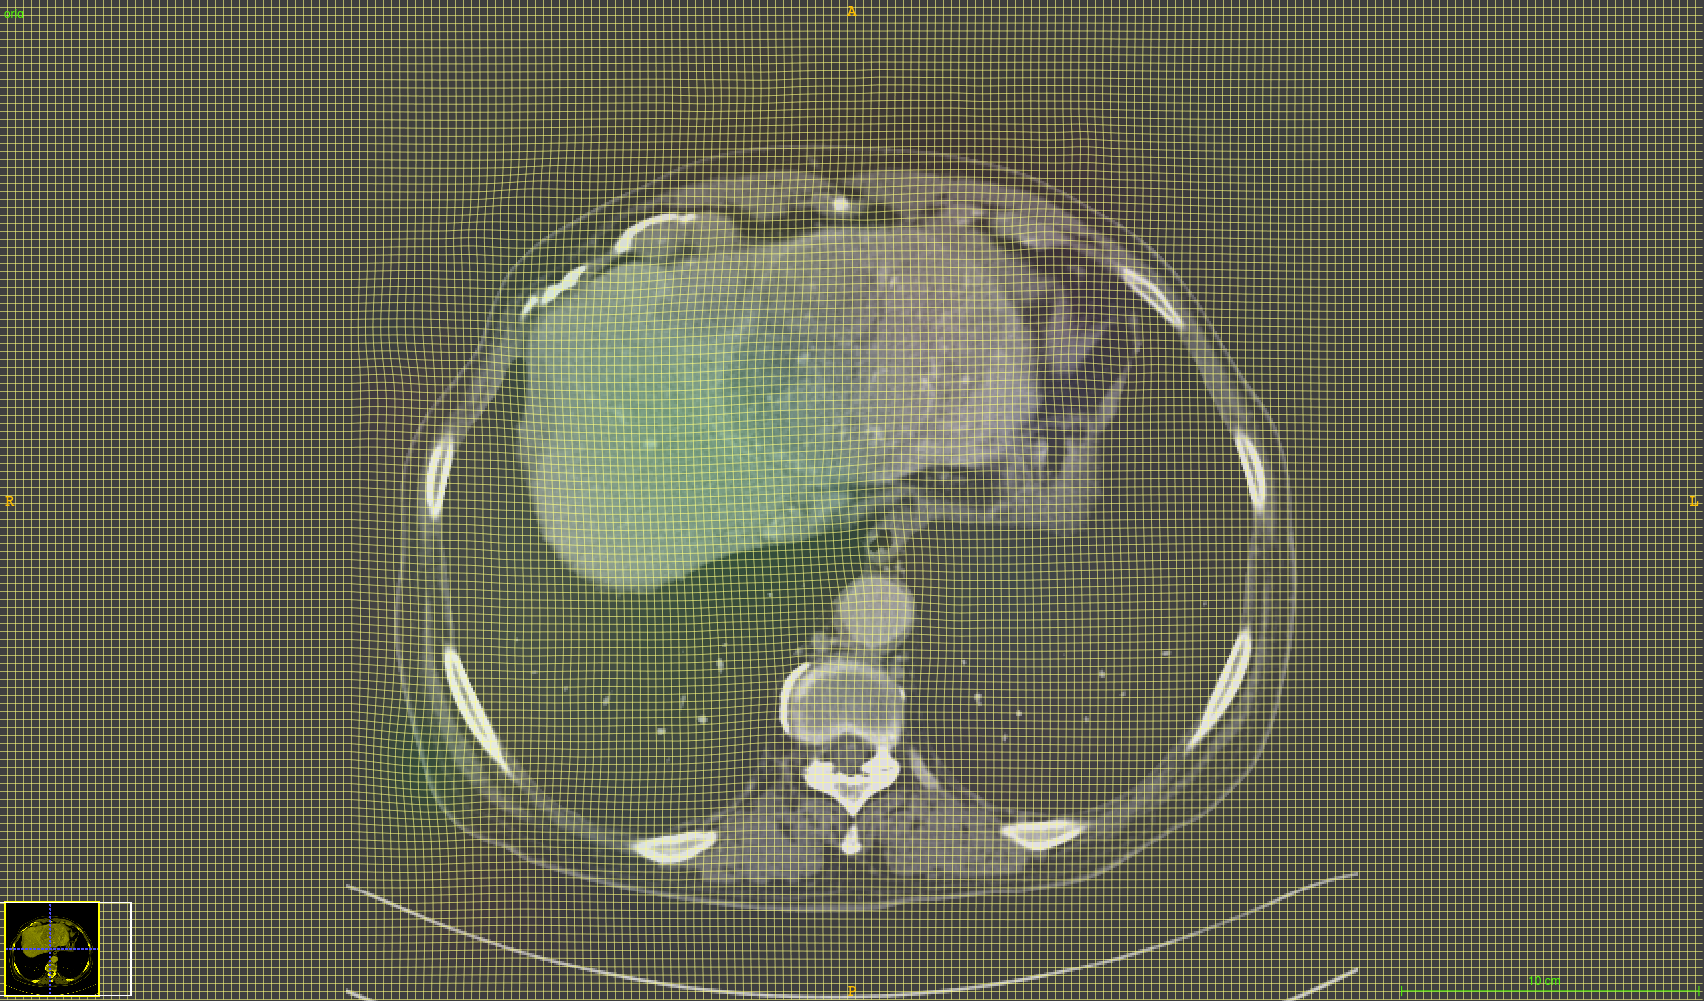
\includegraphics[width=\linewidth]{../HistologicalGradePrediction/images/TCIA_TCGA-DD-A11A_deformation_grid_slice68}
\end{minipage}
\caption{Example of deformation grids obtained after applying the registration pipeline on \lmttfont{TCIA-dB} patients}
\label{fig:deformationGridExamples}
\end{figure}
One way to assess the precision of the registration is to apply the
transformation matrix to the initial resampled \ac{ar} liver mask and to
compute the \ac{dsc} with the target \ac{pv} liver mask. When applying this
evaluation, we obtained a mean patient-wise \ac{dsc} of $ 92.8 \pm 3.8 $ at the
end of the registration step on the \textbf{\lmttfont{TCIA-dB}}, sufficient to consider the
registration as successful when compared with those obtained by state-of-the-art
registration methods applied to the liver \cite{Zhao2019}.

The complete registration pipeline applied to the \textbf{\lmttfont{TCIA-dB}} is detailed in the table \ref{regisPipeline}.

\paragraph{Automatic multiphase tumor segmentation}\label{tcia-db-unsupervised-multiphase-tumor-segmentation}

Once both the \ac{ar} and \ac{pv} volumes of the \textbf{\lmttfont{TCIA-dB}} were registered, and the
liver masks obtained, we built the second step of our cascaded
architecture, dedicated to the multiphasic tumor segmentation. In order
to train such a network, we created a multiphase (arterial and portal
venous) database where the temporal volumes of a given patient are
registered and where segmentations of both the liver and tumor regions
are available.
\textbf{\lmttfont{TheraHCC-dB}} and \textbf{\lmttfont{G-dB}} were the only two datasets containing multiphasic
images (as we can see in table \ref{xp_datasets}), however
\textbf{\lmttfont{G-dB}} initially contained ground truth annotation only for the tumors,
with segmentations performed only on the \ac{ar} phase images.
Since \textbf{\lmttfont{G-dB}} contains more cases than \textbf{\lmttfont{TheraHCC-dB}}, we have decided to
build our multiphasic tumor segmentation network on this dataset.
However in order to train a tumor segmentation network, our cascaded
architecture requires to have the liver segmentation mask as input for
the second step (as depicted in the figure \ref{CARS_DMP_Full_Fig}), therefore we had to obtain the liver segmentation
mask for the patients of the \textbf{\lmttfont{G-dB}}.

\ac{ar} and \ac{pv} volumes of the \textbf{\lmttfont{G-dB}} dataset were initially not registered so
we applied the same registration pipeline as the one used for \textbf{\lmttfont{TCIA-dB}} (see table \ref{regisPipeline}). After application of the procedure to
each patient of \textbf{\lmttfont{G-dB}}, we used the resulting transformation matrix to
transform the \ac{ar} tumor mask to the \ac{pv} space as depicted by the red and green dashed arrows in the figure \ref{fig:GDB_registration_pipeline_vertical}.


\begin{figure}[th!]
\centering
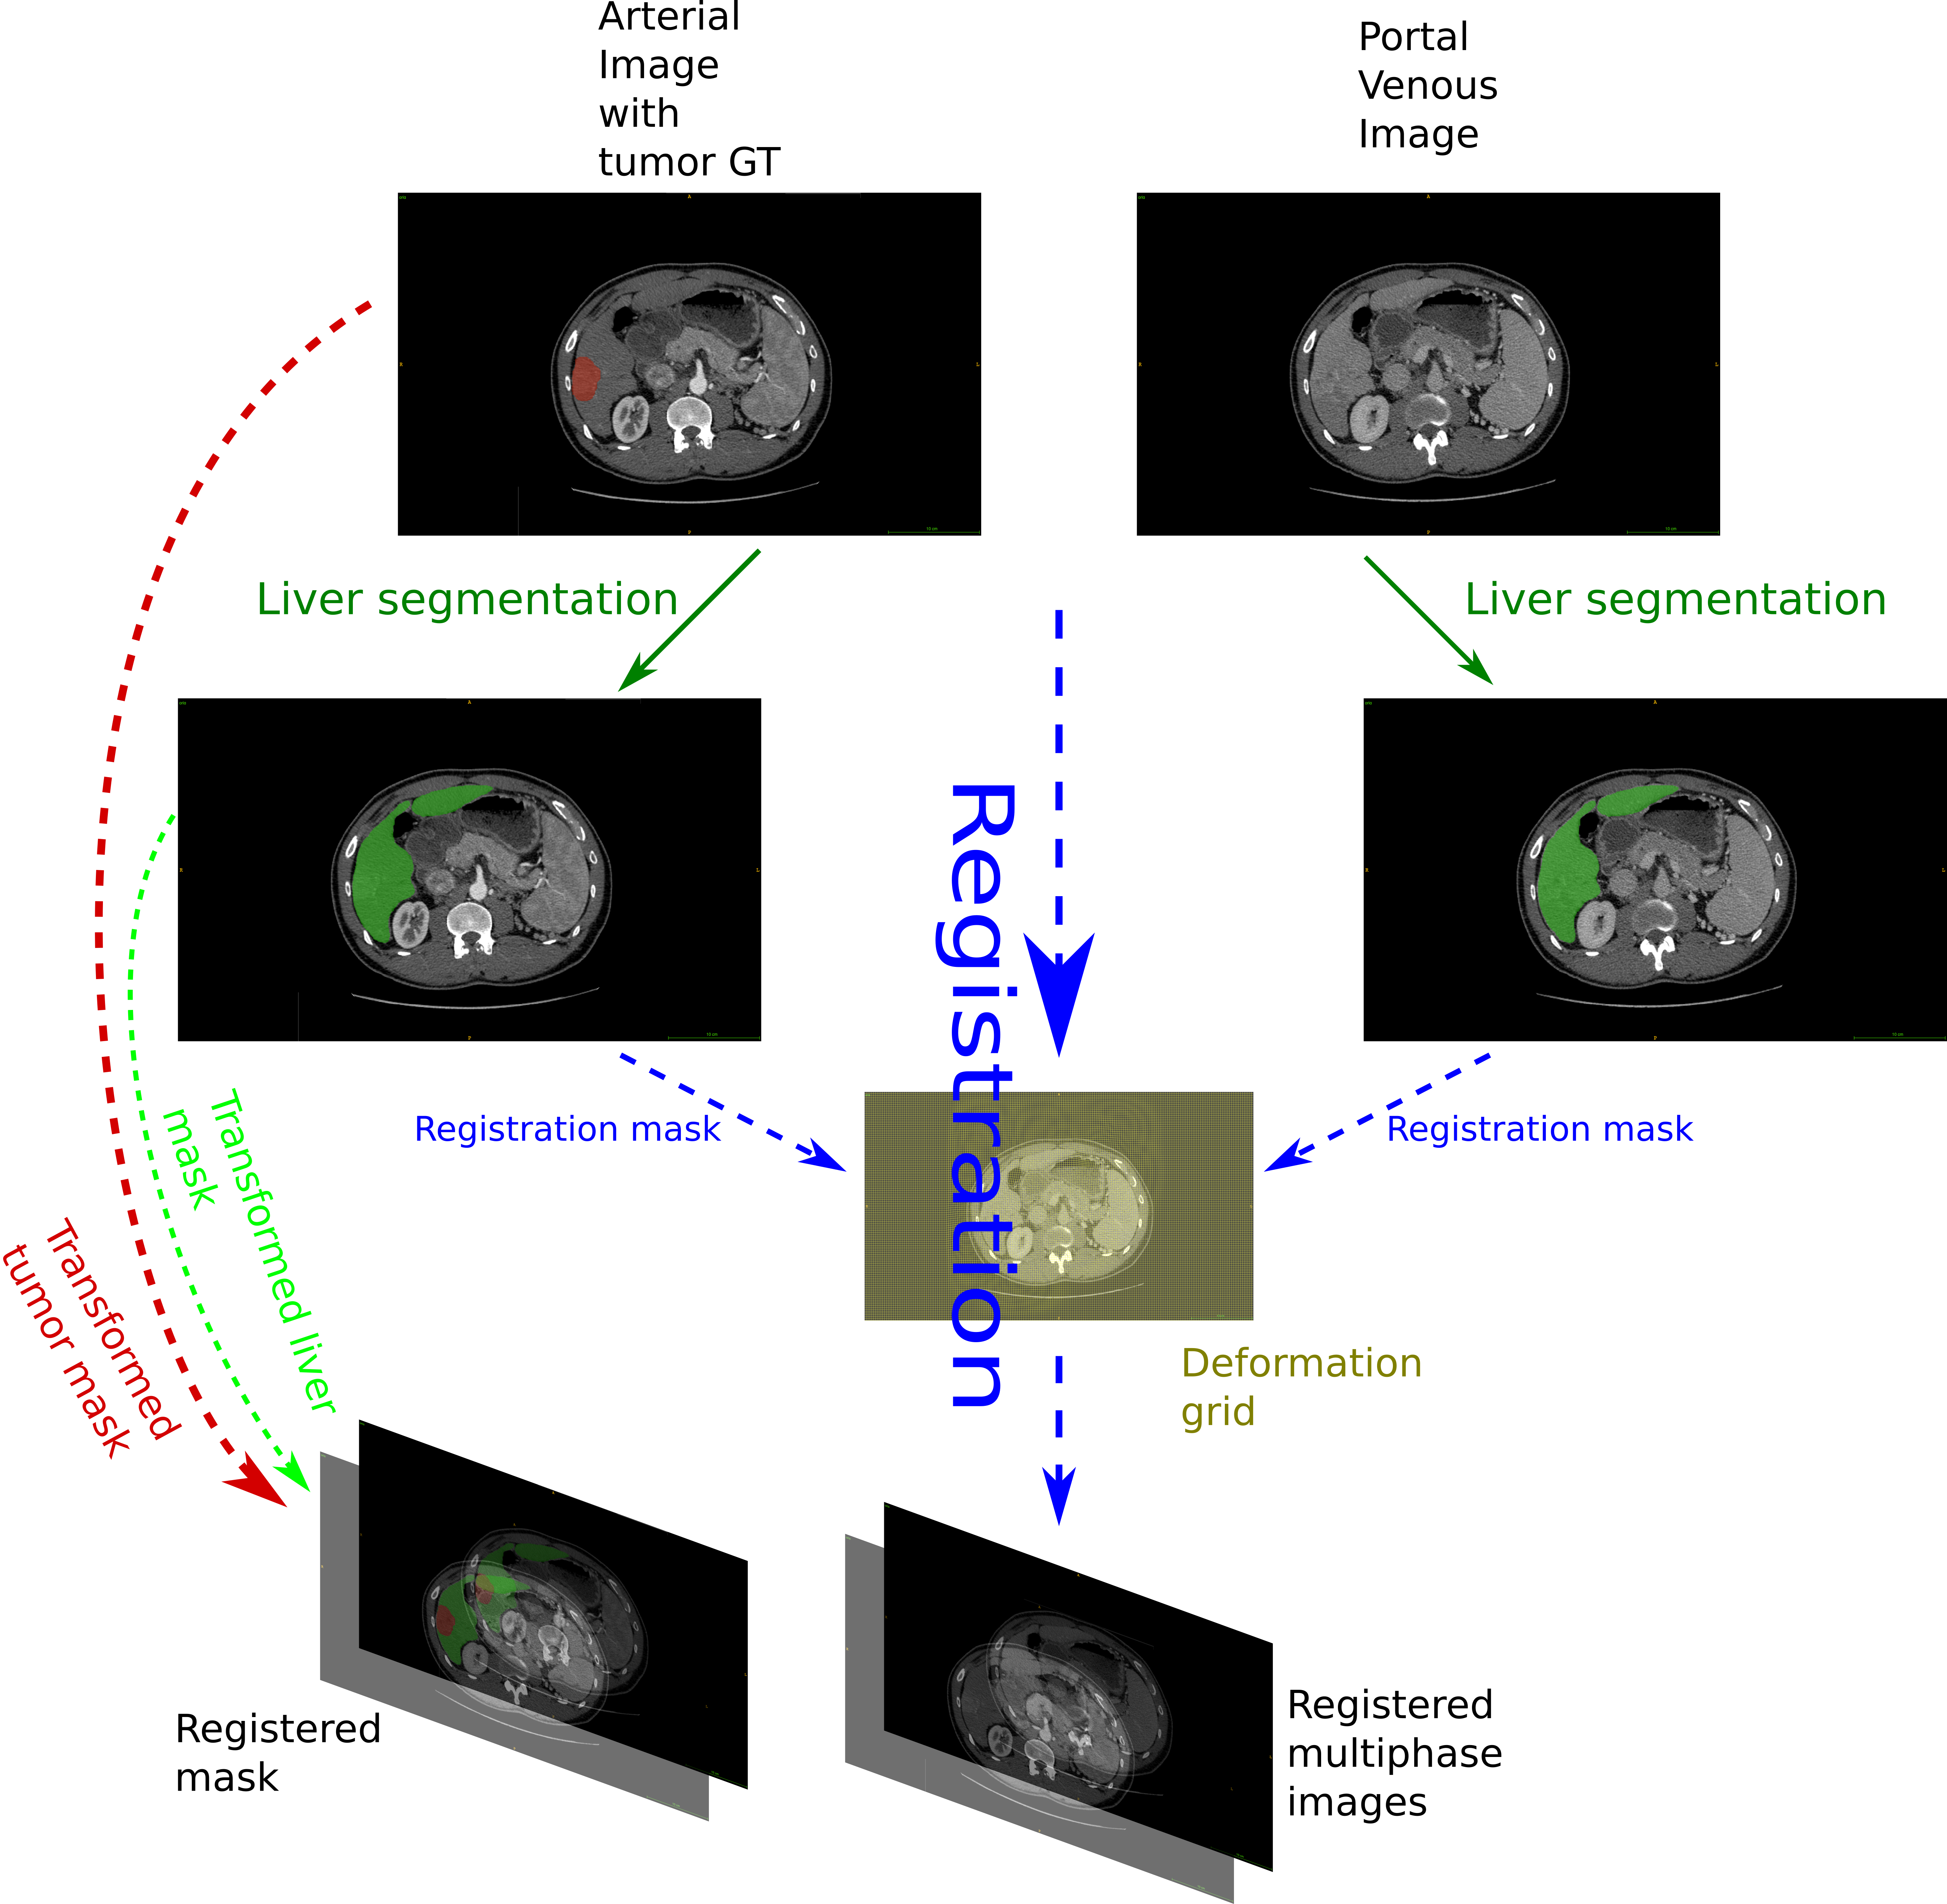
\includegraphics[width=0.9\linewidth]{../HistologicalGradePrediction/images/GDB/GDB_registration_pipeline_vertical}
\caption{Illustration of the registration pipeline applied to \textbf{\lmttfont{G-dB}}. A similar approach as the one applied to \textbf{\lmttfont{TCIA-dB}} is performed to obtain the registered multiphase images. A final step is added here to transform both the tumor and the liver masks using the registration transformation matrix (red and green dashed arrows)}
\label{fig:GDB_registration_pipeline_vertical}
\end{figure}

We then fused the liver and the tumor masks to obtain a multiclass
segmentation mask that can fit both the \ac{pv} and the registered \ac{ar} volumes, as depicted in the figure \ref{fig:gDbRegisteredPatient}.

\begin{figure}[ht!]
\centering
\begin{minipage}{0.45\linewidth}

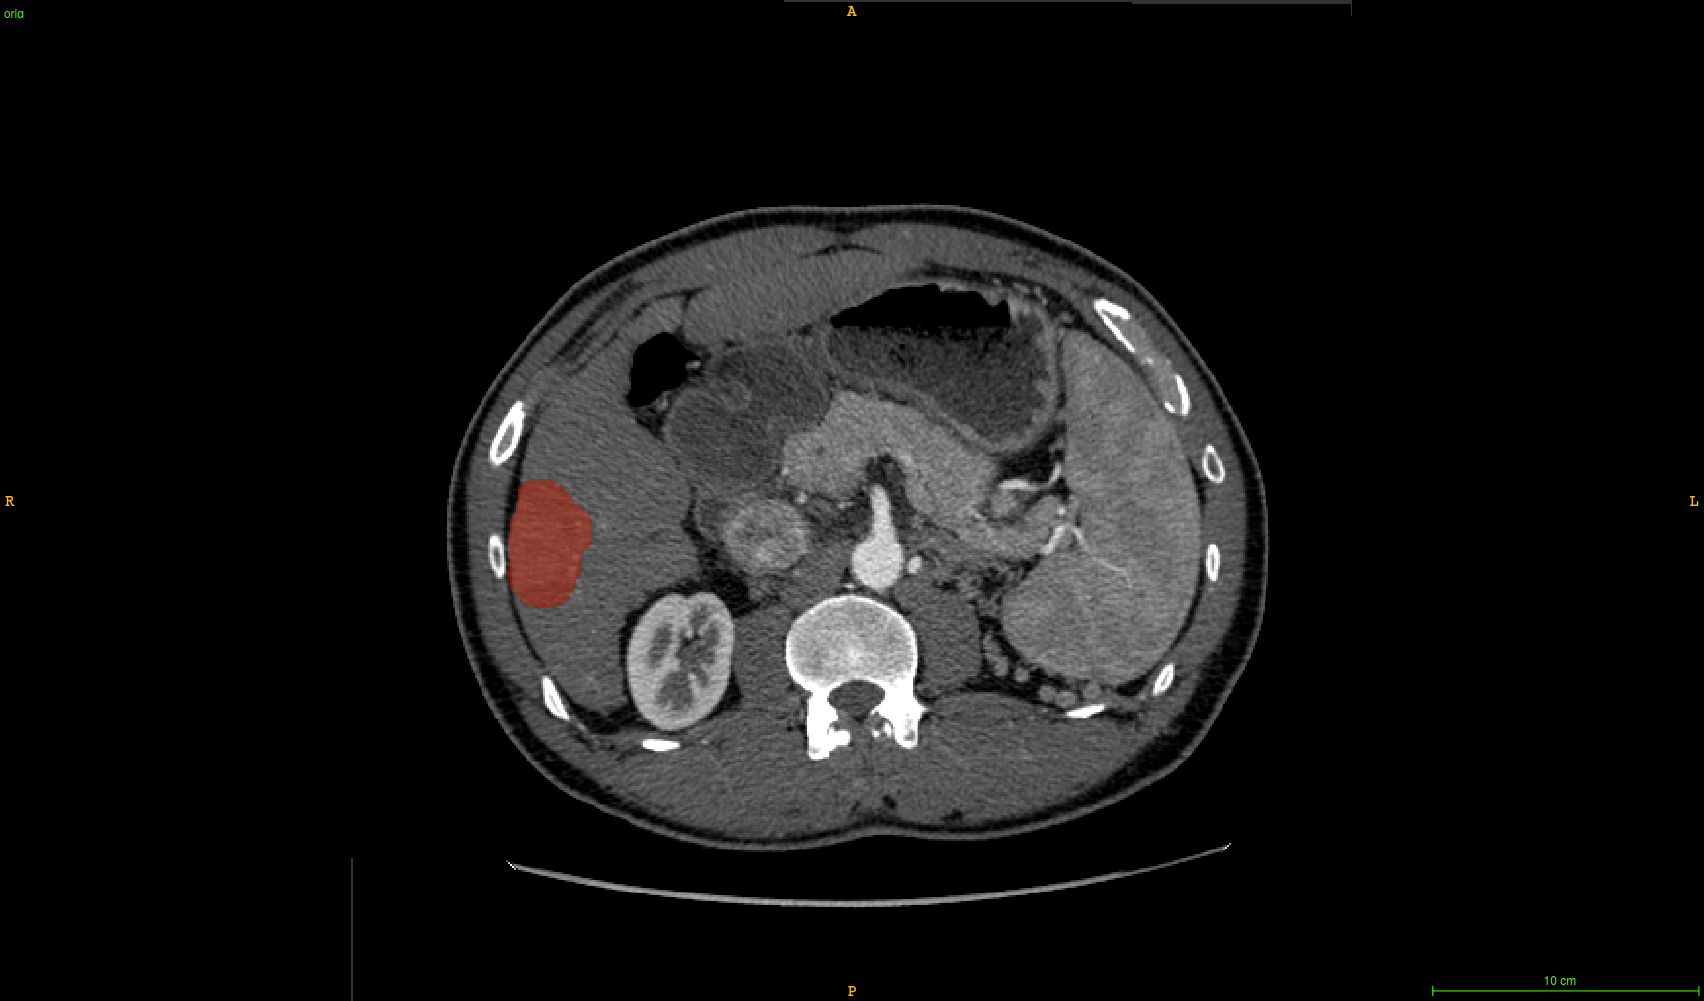
\includegraphics[width=0.9\linewidth]{../HistologicalGradePrediction/images/GDB/GDB_Pat77_slice261_AR_TumorPred}
\end{minipage}
\hspace{0.3cm}
\begin{minipage}{0.45\linewidth}
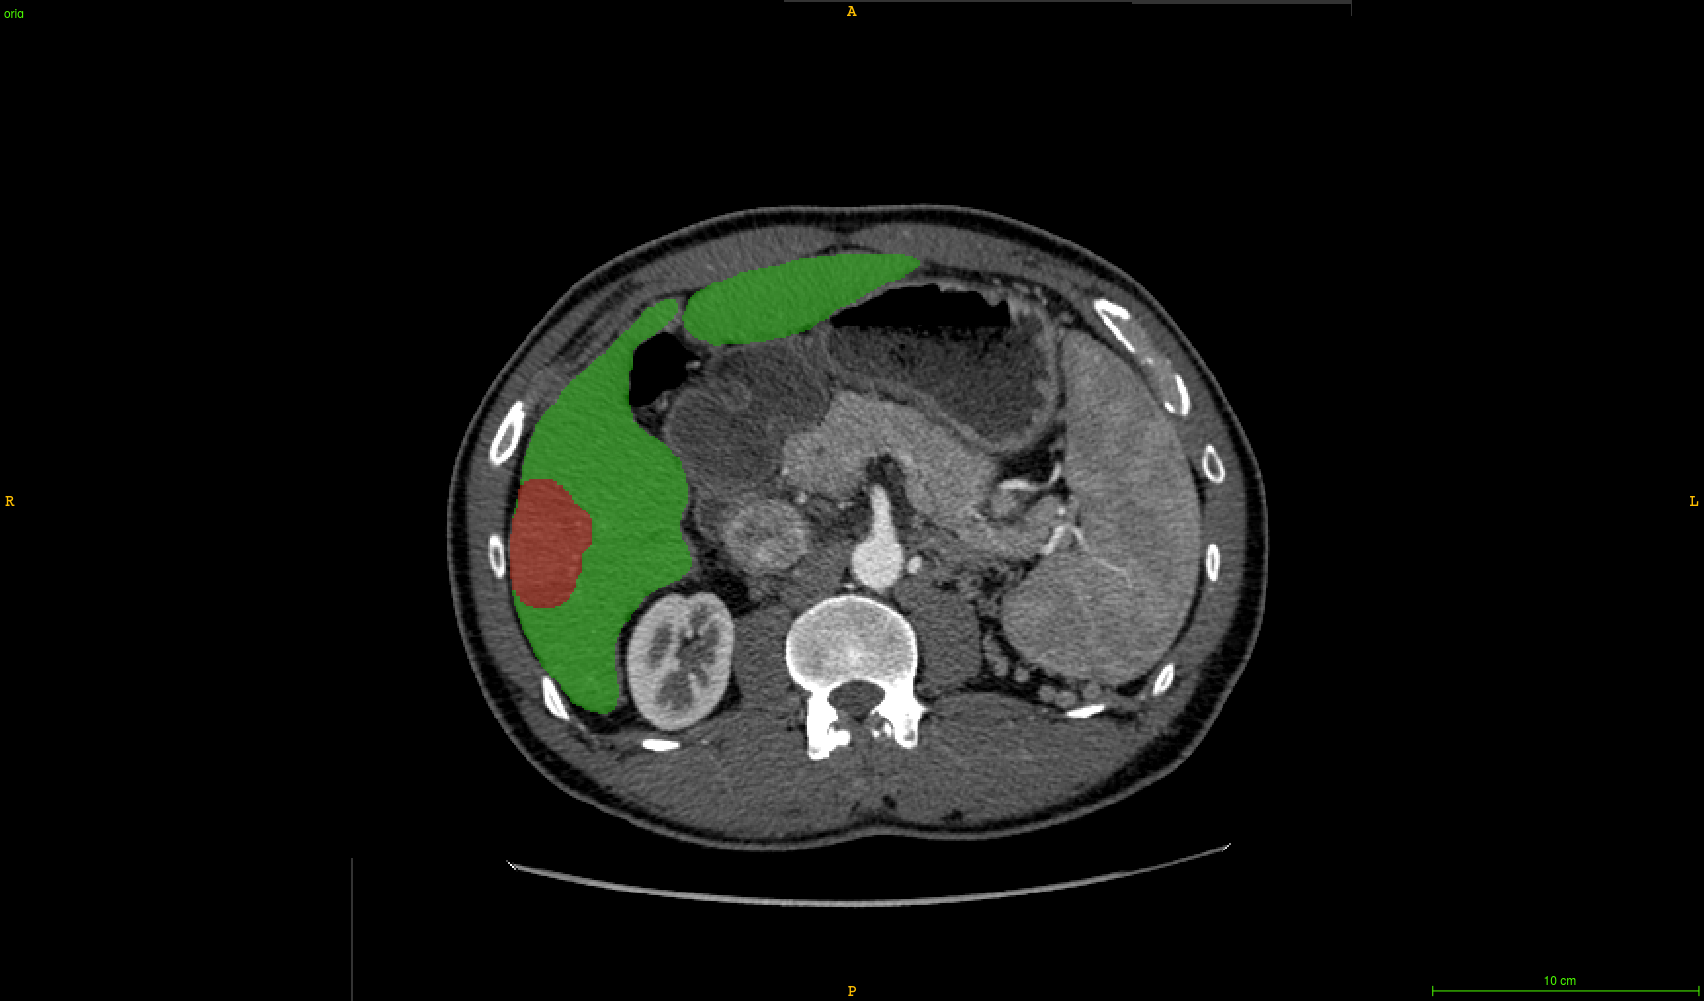
\includegraphics[width=0.9\linewidth]{../HistologicalGradePrediction/images/GDB/GDB_Pat77_slice261_AR_liverTumorPred}
\end{minipage}

\vspace{0.8cm}
\begin{minipage}{0.45\linewidth}
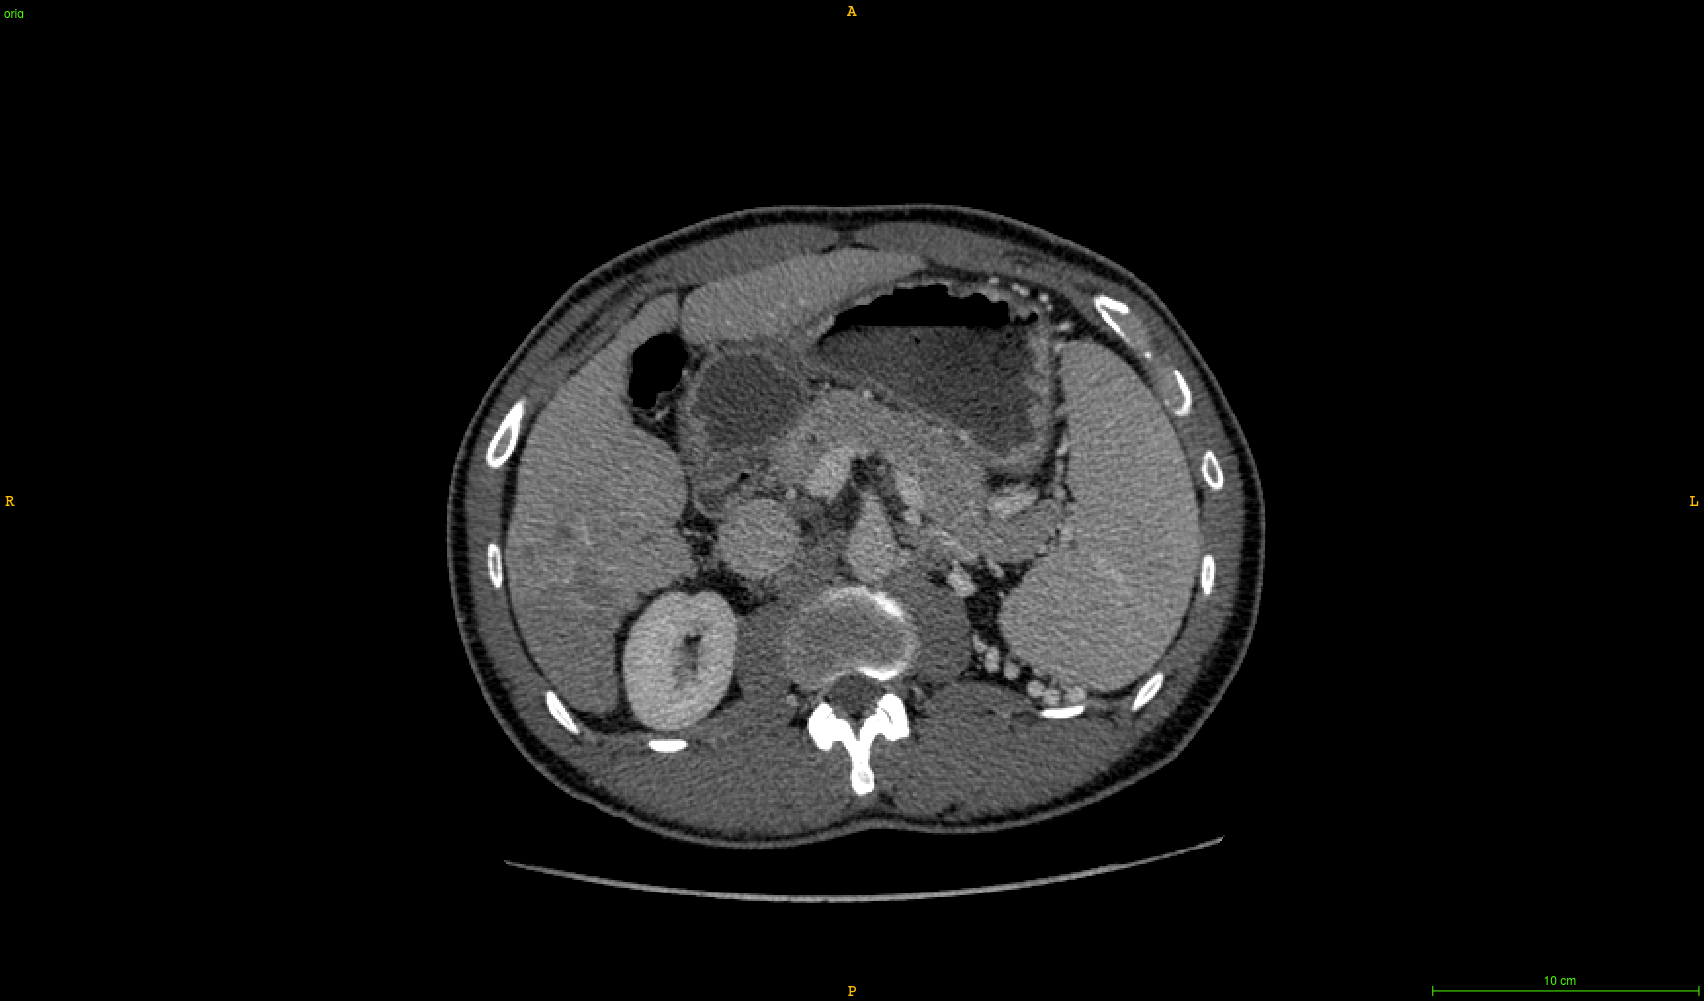
\includegraphics[width=0.9\linewidth]{../HistologicalGradePrediction/images/GDB/GDB_Pat77_slice261_raw_PV}
\end{minipage}
\hspace{0.3cm}
\begin{minipage}{0.45\linewidth}
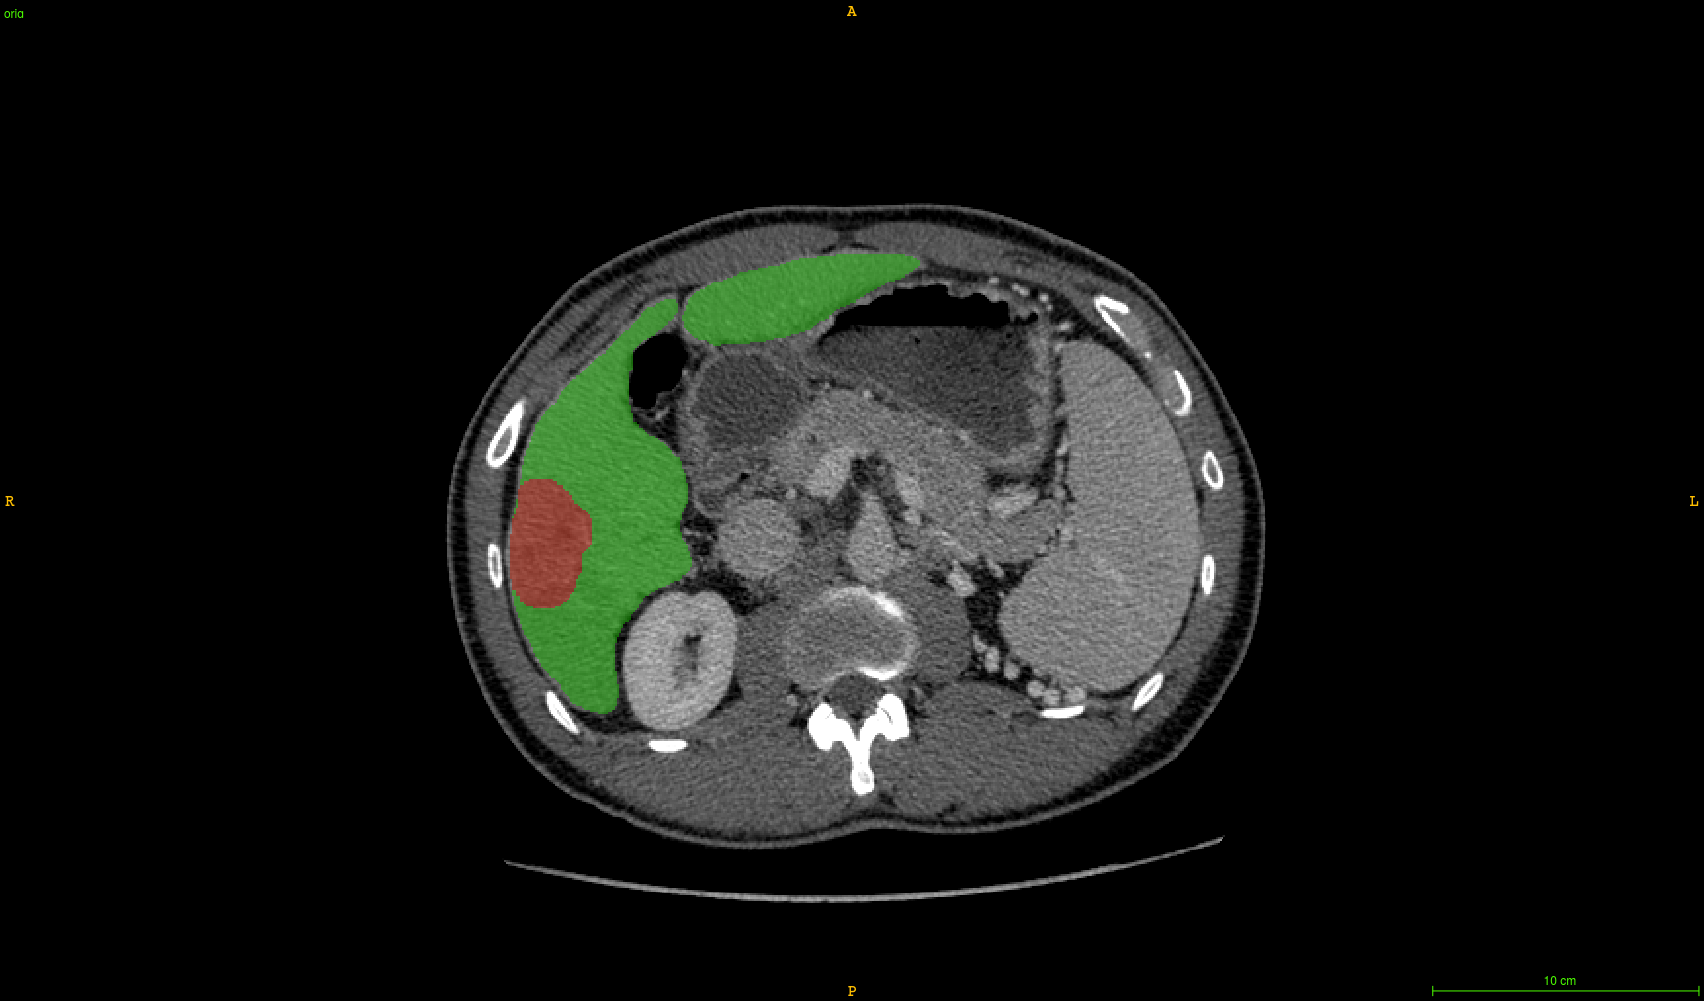
\includegraphics[width=0.9\linewidth]{../HistologicalGradePrediction/images/GDB/GDB_Pat77_slice261_PV_liverTumorPred}
\end{minipage}
\caption{Example of a patient from \textbf{\lmttfont{G-dB}}, obtained after enhancing the dataset with our semantic segmentation network and our registration pipeline. Top row: \ac{ar}\_registered volume with original tumor expert segmentation, bottom row: \ac{pv}\_volume, left: original raw volumes, right: segmentation mask overlay where the parenchyma is obtained through our segmentation pipeline and the tumor was initially delineated by an expert then transformed to fit the target volume space.}
\label{fig:gDbRegisteredPatient}
\end{figure}


We were able thanks to our cascaded architecture and a robust liver
segmentation network to provide additional annotations to the volumes present in \textbf{\lmttfont{G-dB}} that
originally contained only experts annotations for the tumor area on \ac{ar} volumes.

Once a complete database where both the liver and the tumor segmentation
masks were available, and where \ac{ar} and \ac{pv} volumes were registered, we
trained a robust multiphase tumor segmentation network.

We trained both a \pplfont{DMP-Tumor} and a \pplfont{MPF-Tumor} segmentation network on the
registered \textbf{\lmttfont{G-dB}} dataset, and evaluated them on \lmttfont{TCIA-dB} which
contained expert tumor annotations. We evaluated both \pplfont{DMP} and \pplfont{MPF}
architectures since no statistical differences were available when
comparing results obtained for the tumor segmentation in our previous
work on \textbf{\lmttfont{TheraHCC-dB}} \cite{Ouhmich2019}.

After training both architectures with
the same parameters, we obtained a mean patient-wise \ac{dsc} of $ 73.2 \pm 20.6 $ with \pplfont{MPF}
architecture versus $ 64.9 \pm 27.2 $ when using the \pplfont{DMP} when evaluating the
models on the \textbf{\lmttfont{TCIA-dB}} patients. An example of prediction on the \textbf{\lmttfont{TCIA-dB}} is
depicted in figure \ref{fig:TCIAMultiphaseTumorPred}.

\begin{figure}
\begin{minipage}{0.3\linewidth}
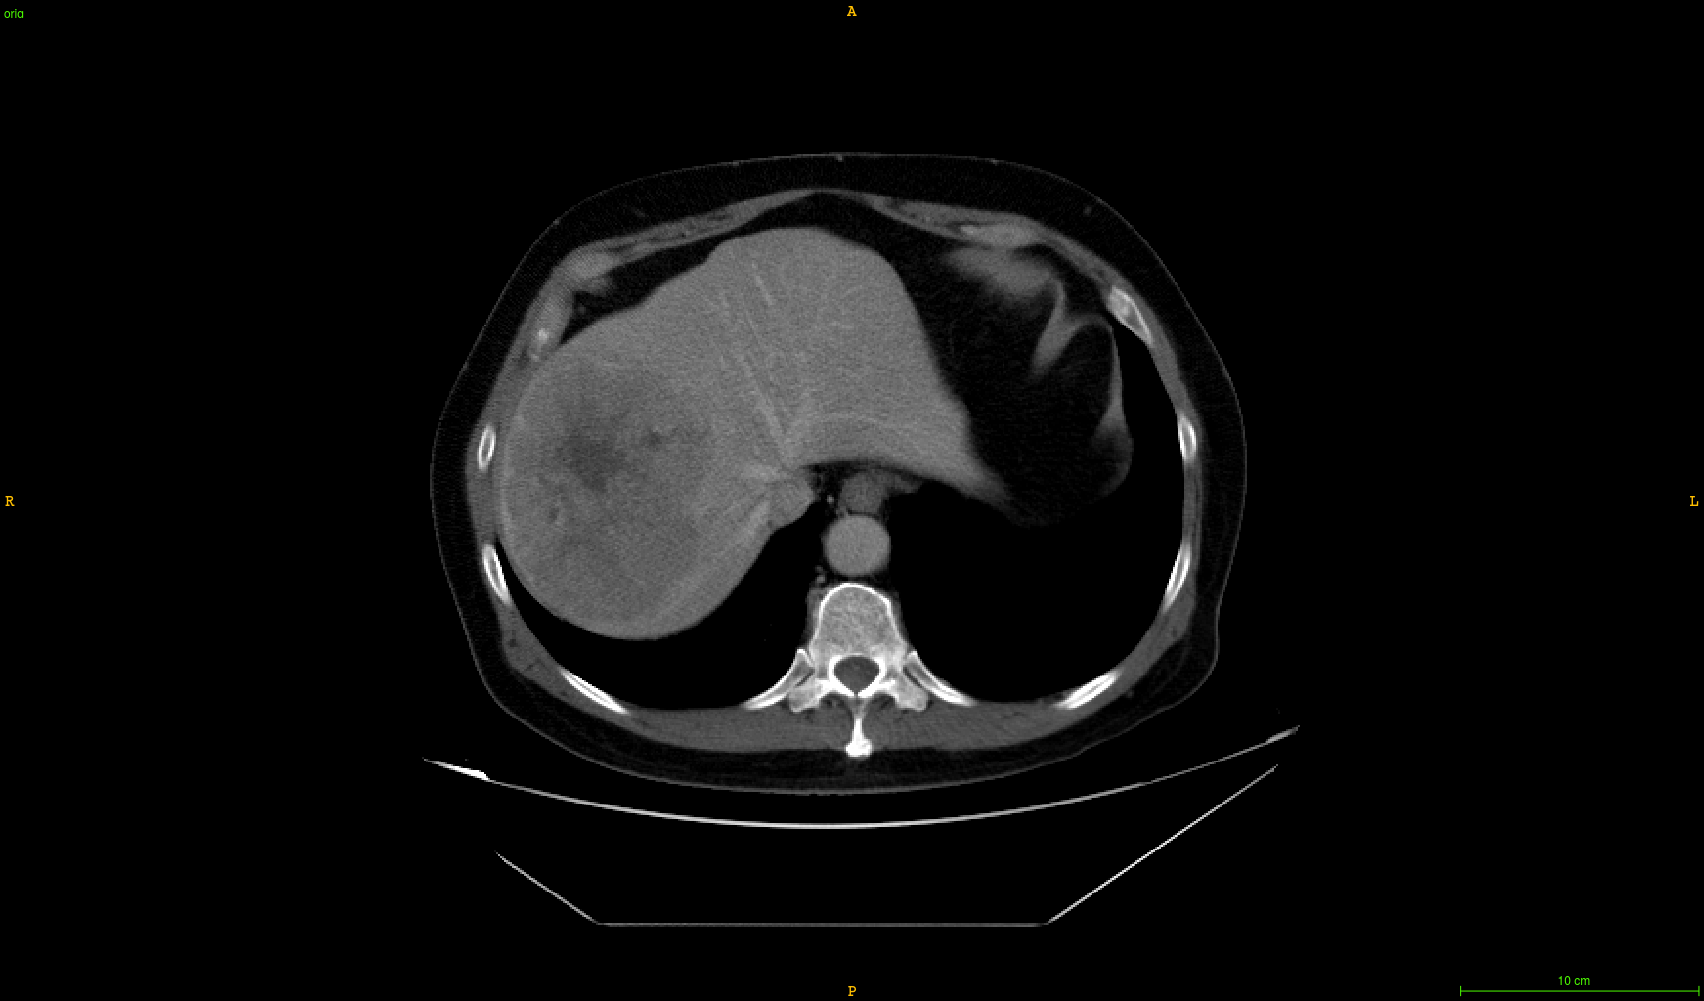
\includegraphics[width=\linewidth]{../HistologicalGradePrediction/images/image13.png}
\end{minipage}
\hspace{0.1cm}
\begin{minipage}{0.3\linewidth}
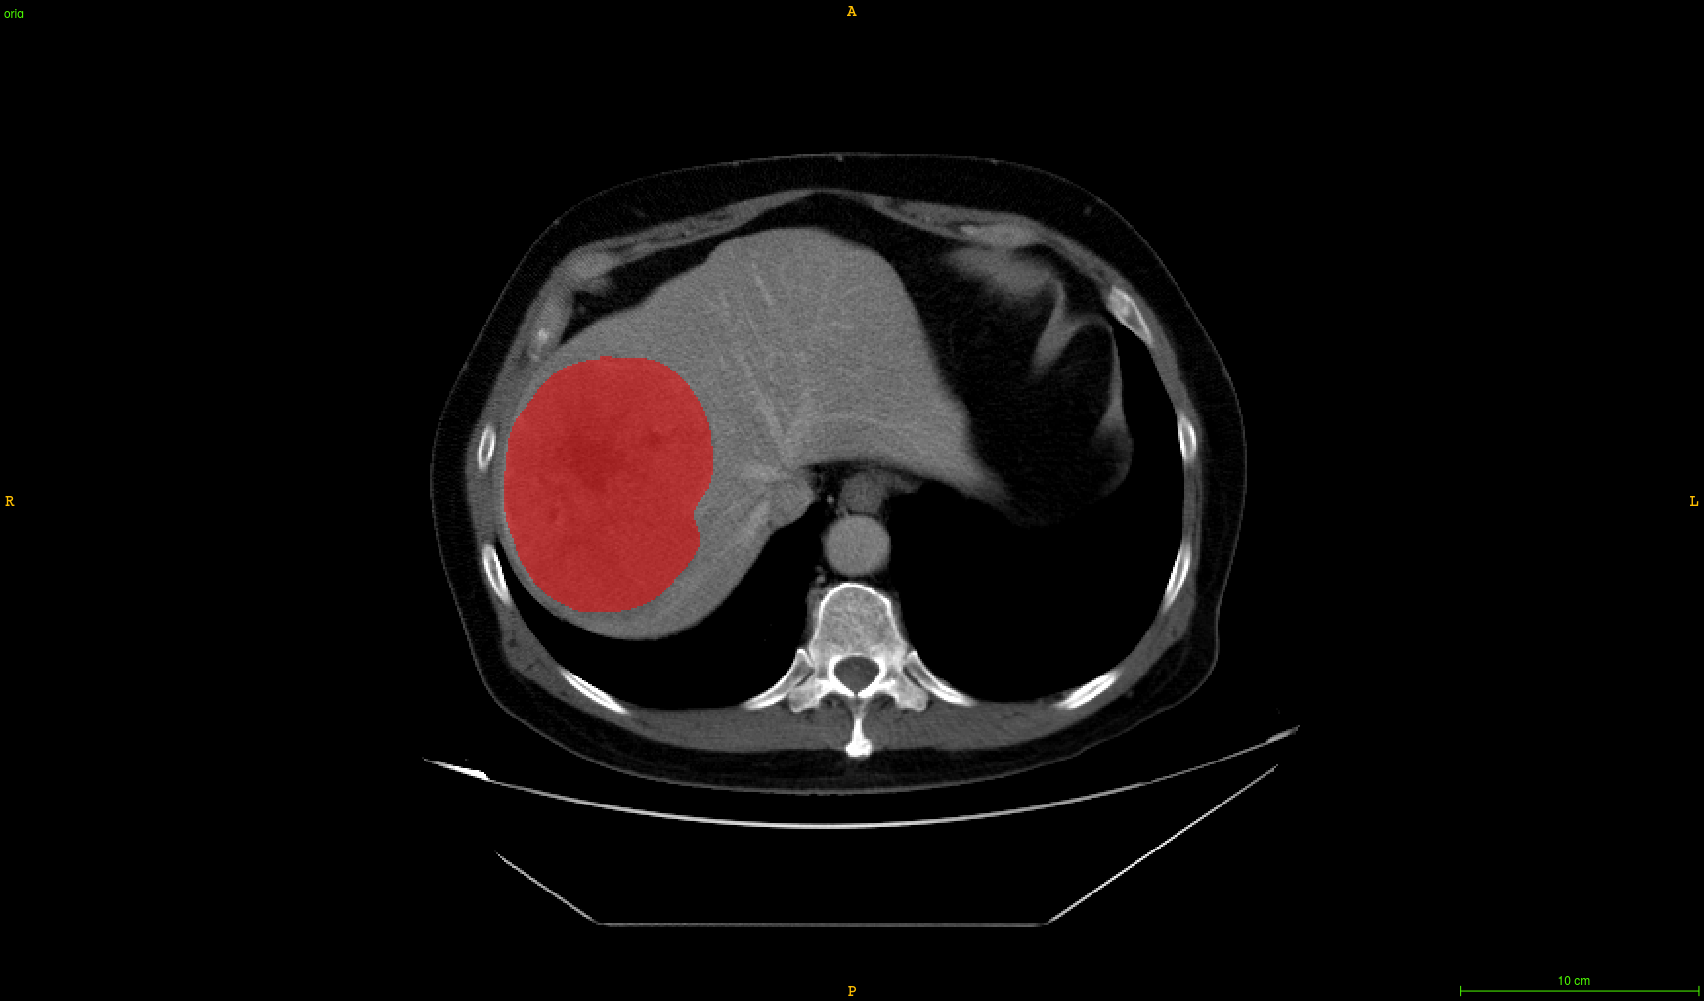
\includegraphics[width=\linewidth]{../HistologicalGradePrediction/images/image10.png}
\end{minipage}
\hspace{0.1cm}
\begin{minipage}{0.3\linewidth}
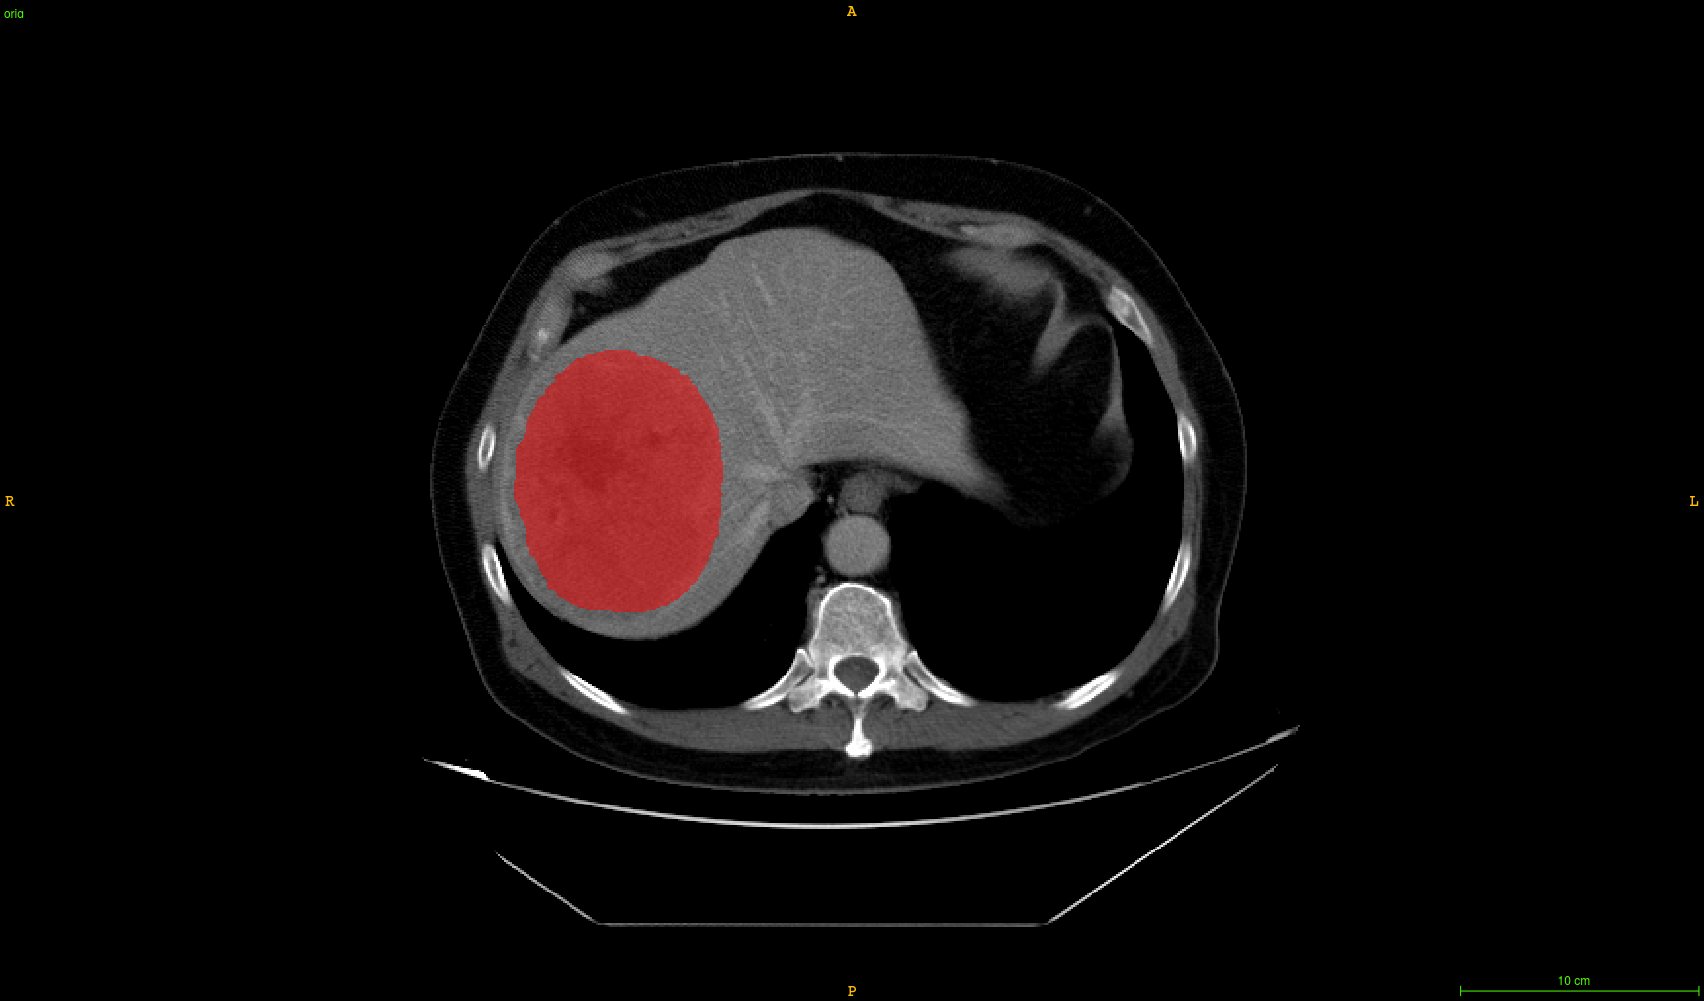
\includegraphics[width=\linewidth]{../HistologicalGradePrediction/images/image7.png}
\end{minipage}
\caption{Example of an image from the \textbf{\lmttfont{TCIA-dB}}, with the obtained predicted tumor
segmentation using the \pplfont{MPF-Tumor} segmentation network (left: raw,
middle: expert annotation, right: obtained segmentation)}
\label{fig:TCIAMultiphaseTumorPred}
\end{figure}


Those results obtained on an external dataset tend to demonstrate a satisfactory precision
of the tumor segmentation when training a cascaded architecture with a
sufficient number of cases.
We retained the \pplfont{MPF-Tumor} segmentation network since it performed
significantly better than the \pplfont{DMP} one ($ p = 0.02 $ using a Wilcoxon signed
paired rank test on the patient-wise \ac{dsc}).
We confirmed the benefit of the cascaded architecture since these results
were obtained using an architecture where the first network was trained
on \textbf{\lmttfont{LITS-dB}} and the second on \textbf{\lmttfont{G-dB}}. We were also able to use
a monophase network for the first step and a multiphasic network for the
second.
This work proved the ability of deep learning (semantic segmentation
network) combined with image processing (registration) to enhance and
complete weakly annotated databases (both \textbf{\lmttfont{TCIA-dB}} and \textbf{\lmttfont{G-dB}} were
enhanced in the same way).

%Finally, we decided to keep only two stages in our cascaded architecture
%since the only available dataset with expert necrosis annotation was the
%\lmttfont{TheraHCC-dB}, containing only 7 patients. This small amount of cases
%combined with the design of \lmttfont{TheraHCC-dB} (only sparse slices are
%annotated across the volume) might not be enough to precisely
%differentiate between the active and the necrotic part of the lesions on
%unseen cases. Moreover, the necrosis segmentation appears to be more
%sensitive than the tumor segmentation, especially because the necrosis
%requires separate annotations in each phase (in case of \ac{ar} and \ac{pv} volumes) since necrotic tissues will respond differently to the evolution of contrast medium.



\section{Deep Radiomics for histological grade prediction}

\subsection{Introduction}\label{introduction}

The main goal of our work is to use imaging features to better characterize the liver cancers.
We decided to extract relevant imaging features from our multiphase cascaded semantic segmentation
to perform the prediction of histological grade.
The prediction of the histological grade of the tumor was rarely studied, since only one study
used deep learning tools to perform this task but with MR images as
input \cite{Yang2019}.
Indeed, this task appears to be more challenging than previous \ac{dlr}
liver-related work where either the type of \ac{fll} or the treatment
response (such as the recurrence) were predicted (\textbf{see section \ref{deep-learning-radiomics}}).\\
We will now focus on the only study in the literature that tackled the
problem of predicting the histological grade of \ac{hcc}s through a \ac{dl}
architecture with medical images, before presenting our own automatic \ac{dl}
pipeline.

\subsection{Related work}\label{dlr-based-study-to-predict-the-histological-hcc-grade}

To our knowledge, only one study tackled the problem of estimating the
histological grade of \ac{hcc}s using a \ac{dl} architecture, but with MR images
as input \cite{Yang2019}.

Yang et al. incorporated 42 patients suffering from \ac{hcc} in their study,
resulting in a total of 51 \ac{hcc}s. Each lesion was analyzed by 2
experienced pathologists who estimated their histological grade after
microscopic examination (the lesions were classified as well, moderately
and poorly differentiated, following the WHO classification system \cite{20113051318}) .
The extracted tissues were obtained through either biopsy (12 patients)
or after surgical removal (2 liver transplants and 28 liver resection).
All the 42 patients underwent pre-operative multiphasic MR imaging
examinations and images were available at 5 different phases
(precontrast, late arterial, portal venous, equilibrium and delayed
phases). They obtained a dataset composed of 9 well, 7 poorly and 35 moderately
differentiated \ac{hcc}s.

For each patient, a \ac{roi} was placed by one expert at the maximal axial
cross-sectional area to entirely cover the tumor. The \ac{roi} was
copied in the 2 slices above and below the chosen one, to obtain a 3D
volume. Intensities of each volume were normalized and 4D tensors were
created for each patient so that each tensor had a $ 32\times32\times5\times5 $ shape
($ 32\times32 $ corresponding to the resampled axial \ac{roi} dimension, the third
dimension being the number of retained slices, and the last dimension being the
dynamic temporal evolution of the \ac{roi} with the 5 phases).

The used architecture is depicted in the figure \ref{fig:Yang2019_Figure2_MCF-3DCNN}. It first splits the 4D
tensors into 5 3D objects so that each slice is treated separately. Each
3D volume was then processed by 2 convolutional, 2 max pooling and 1
fully connected layer. The features of each slice were then
concatenated, before a second fully connected layer followed by a dense
layer with a softmax activation function outputs the probability of
belonging to each one of the three classes (well, moderately or poorly differentiated).

\begin{figure}[th!]
\centering
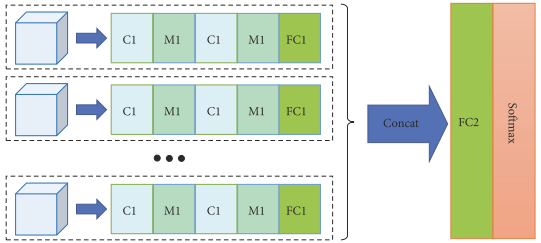
\includegraphics[width=0.7\linewidth]{../HistologicalGradePrediction/images/Yang2019_Fig2}
\caption{MCF-3DCNN architecture as detailed by \textbf{©Yang et al. \cite{Yang2019}}}
\label{fig:Yang2019_Figure2_MCF-3DCNN}
\end{figure}


During the training process, they implemented a label-shuffling method
to overcome the problem of imbalanced data. Furthermore, to avoid the
effect of overfitting, they trained their network with augmented data
(original images were transposed, rotated, and flipped), a learning rate
reduction and the addition of dropout (rate = 0.5).
Using their architecture they were able to correctly classify the \ac{hcc}s
into the 3 differentiation groups with a mean accuracy of \textbf{74\%}.\\
Their study however suffers from a lot of limitations such as the
reduced size of the cohort, the imbalanced data and the fact that the
analysis was only performed in a manually drawn \ac{voi}.\\
We have decided to tackle the same issue, but we implemented a fully
automatic pipeline where both the segmentation and the grade prediction
steps were performed by \ac{dl} networks.


\subsection{Prediction of the histological grade}\label{prediction-of-the-histological-grade-on-tcia-db}

In order to perform the prediction of the histological grade, our idea
is to use the imaging features retained for the liver tissue
segmentation, especially those used to segment tumoral structures.
We believe that one easy way to extract relevant imaging features is to
use those retained by the semantic segmentation networks, thus the
better the accuracy regarding the semantic segmentation of the liver
tissues, the more accurate the histological grade prediction will be.
As explained previously, we proved that a cascaded architecture combined
with the use of temporal contrast enhanced images allows a better
delineation of liver tissues. We therefore proved that the designed cascaded architecture can be applied to provide missing annotations into weakly annotated datasets such as \textbf{\lmttfont{TCIA-dB}}.
It has been proven that using temporal information can improve the accuracy of the grade prediction, by exploiting the wash-in wash-out specific features \cite{Okamoto2012}.
To conduct our \ac{dlr} study, we first performed a multiphasic
semantic segmentation of the \textbf{\lmttfont{TCIA-dB}}, before predicting the
histological grade.
After obtaining the final cascaded architecture, we built our network dedicated to the
histological grade prediction.

\subsubsection{Experiments and results}

\lmttfont{TCIA-dB} contains images from 18 patients, where 9 were diagnosed with a
grade 3 (G3), 7 with a grade 2 (G2) and 2 with a grade 1 (G1). In order
to obtain a balanced training dataset, it has been decided to split them
into two groups, the first containing G1 and G2 patients, and the second containing G3 patients, as it has been done previously in the literature since G2
was considered as being closer to G1 than to G3 \cite{Han2013,Zucman-Rossi2015}. Patients from the first group (G1 and G2) were considered as
having a low grade (LG), whereas those from the second group have a high
grade (HG).
As explained previously, to train a network dedicated to predict the
histological grade, we have decided to focus on what we called the
relevant imaging semantic features.
We therefore extracted the features from the second network of our
cascaded architecture, to focus on the temporal behavior of the tumor.

The retained network (\pplfont{MPF-Tumor} architecture as illustrated in the figure \ref{CARS_MPF_Full_Fig}) is made of 2 classical U-Net networks, where each
one takes either the \ac{ar} or the \ac{pv} image as input. We believe
that the compressed information present in the bottleneck part of the
network can be sufficient to encode the useful information present in the
image (the U-Net will work as an auto-encoder for the semantic information). Therefore, we extracted for each patient of the \textbf{\lmttfont{TCIA-dB}}, this
encoded information in a slice-wise manner, represented by two $ 32\times32\times512 $
features cubes (one per phase in the \pplfont{MPF-Tumor} architecture) per slice
as depicted in the figure \ref{fig:MPF_Features_Selection}.


\begin{figure}[th!]
\centering
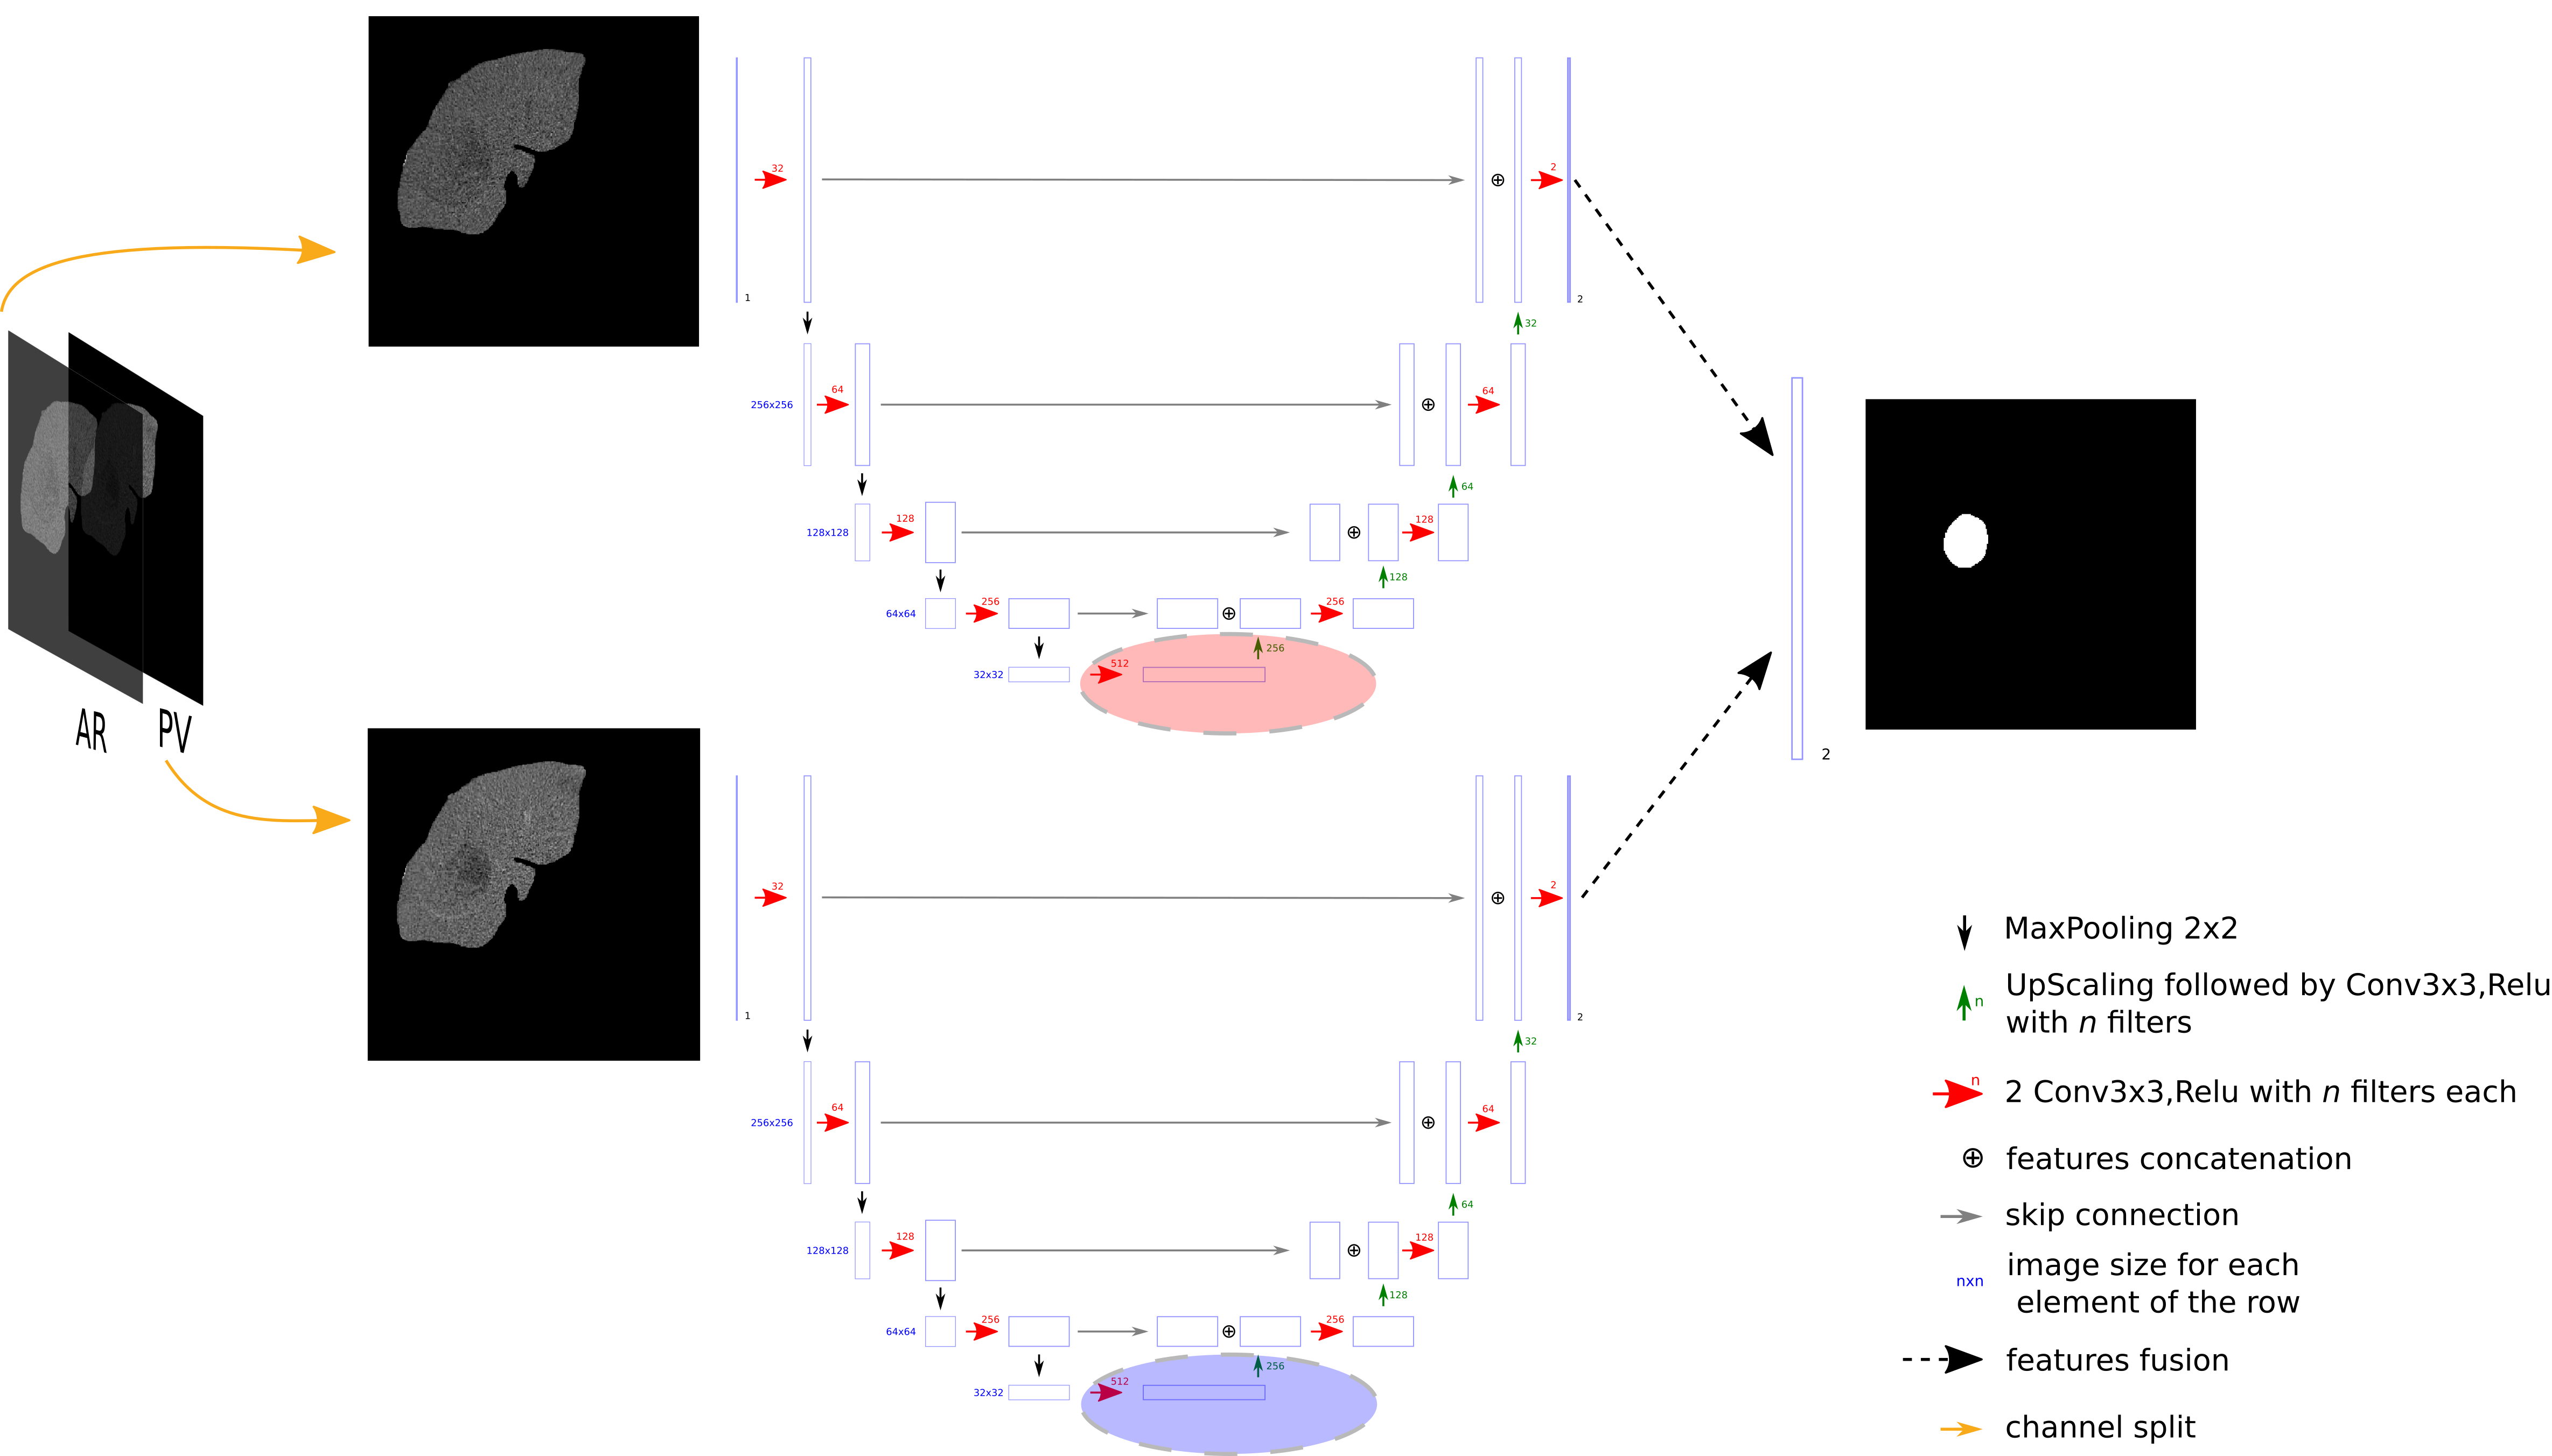
\includegraphics[width=0.95\linewidth]{../HistologicalGradePrediction/images/MPF_Features_Selection}
\caption{Red and blue areas correspond to the bottleneck part of the U-Net
network where the features extraction is performed. Each image is then
represented as a $ 32\times32\times512 $ features cube.}
\label{fig:MPF_Features_Selection}
\end{figure}


Before applying the extraction of the features, we normalized
the dimension of the different volumes of the dataset, so that each
voxel measures $ 0.68\times0.68 $mm in the axial plane (because it corresponds to
the resolution of the images used to train our semantic segmentation
network), and that the volumes have a 2.5mm z-spacing (corresponding to the
spacing of the majority of the \ac{pv} volumes in \textbf{\lmttfont{TCIA-dB}}).

We finally built an architecture responsible for the grade prediction.
We focused only on the centrally located tumor slices, since the
histological grade corresponds to a measurement of the evolution of the
disease, which tends to have more physiological effects at the center of
the tumor. Centrally located slices will therefore exhibit the highest
grade for a given patient.

Therefore, a slice-wise architecture was built, first because the
features were computed in a slice-wise manner and second because the
histological grade tends to be heterogeneous in the lesion, meaning that
a slice-wise approach allows us to give a finer prediction to find
potential areas with a more advanced disease.


\begin{figure}[th!]
\centering
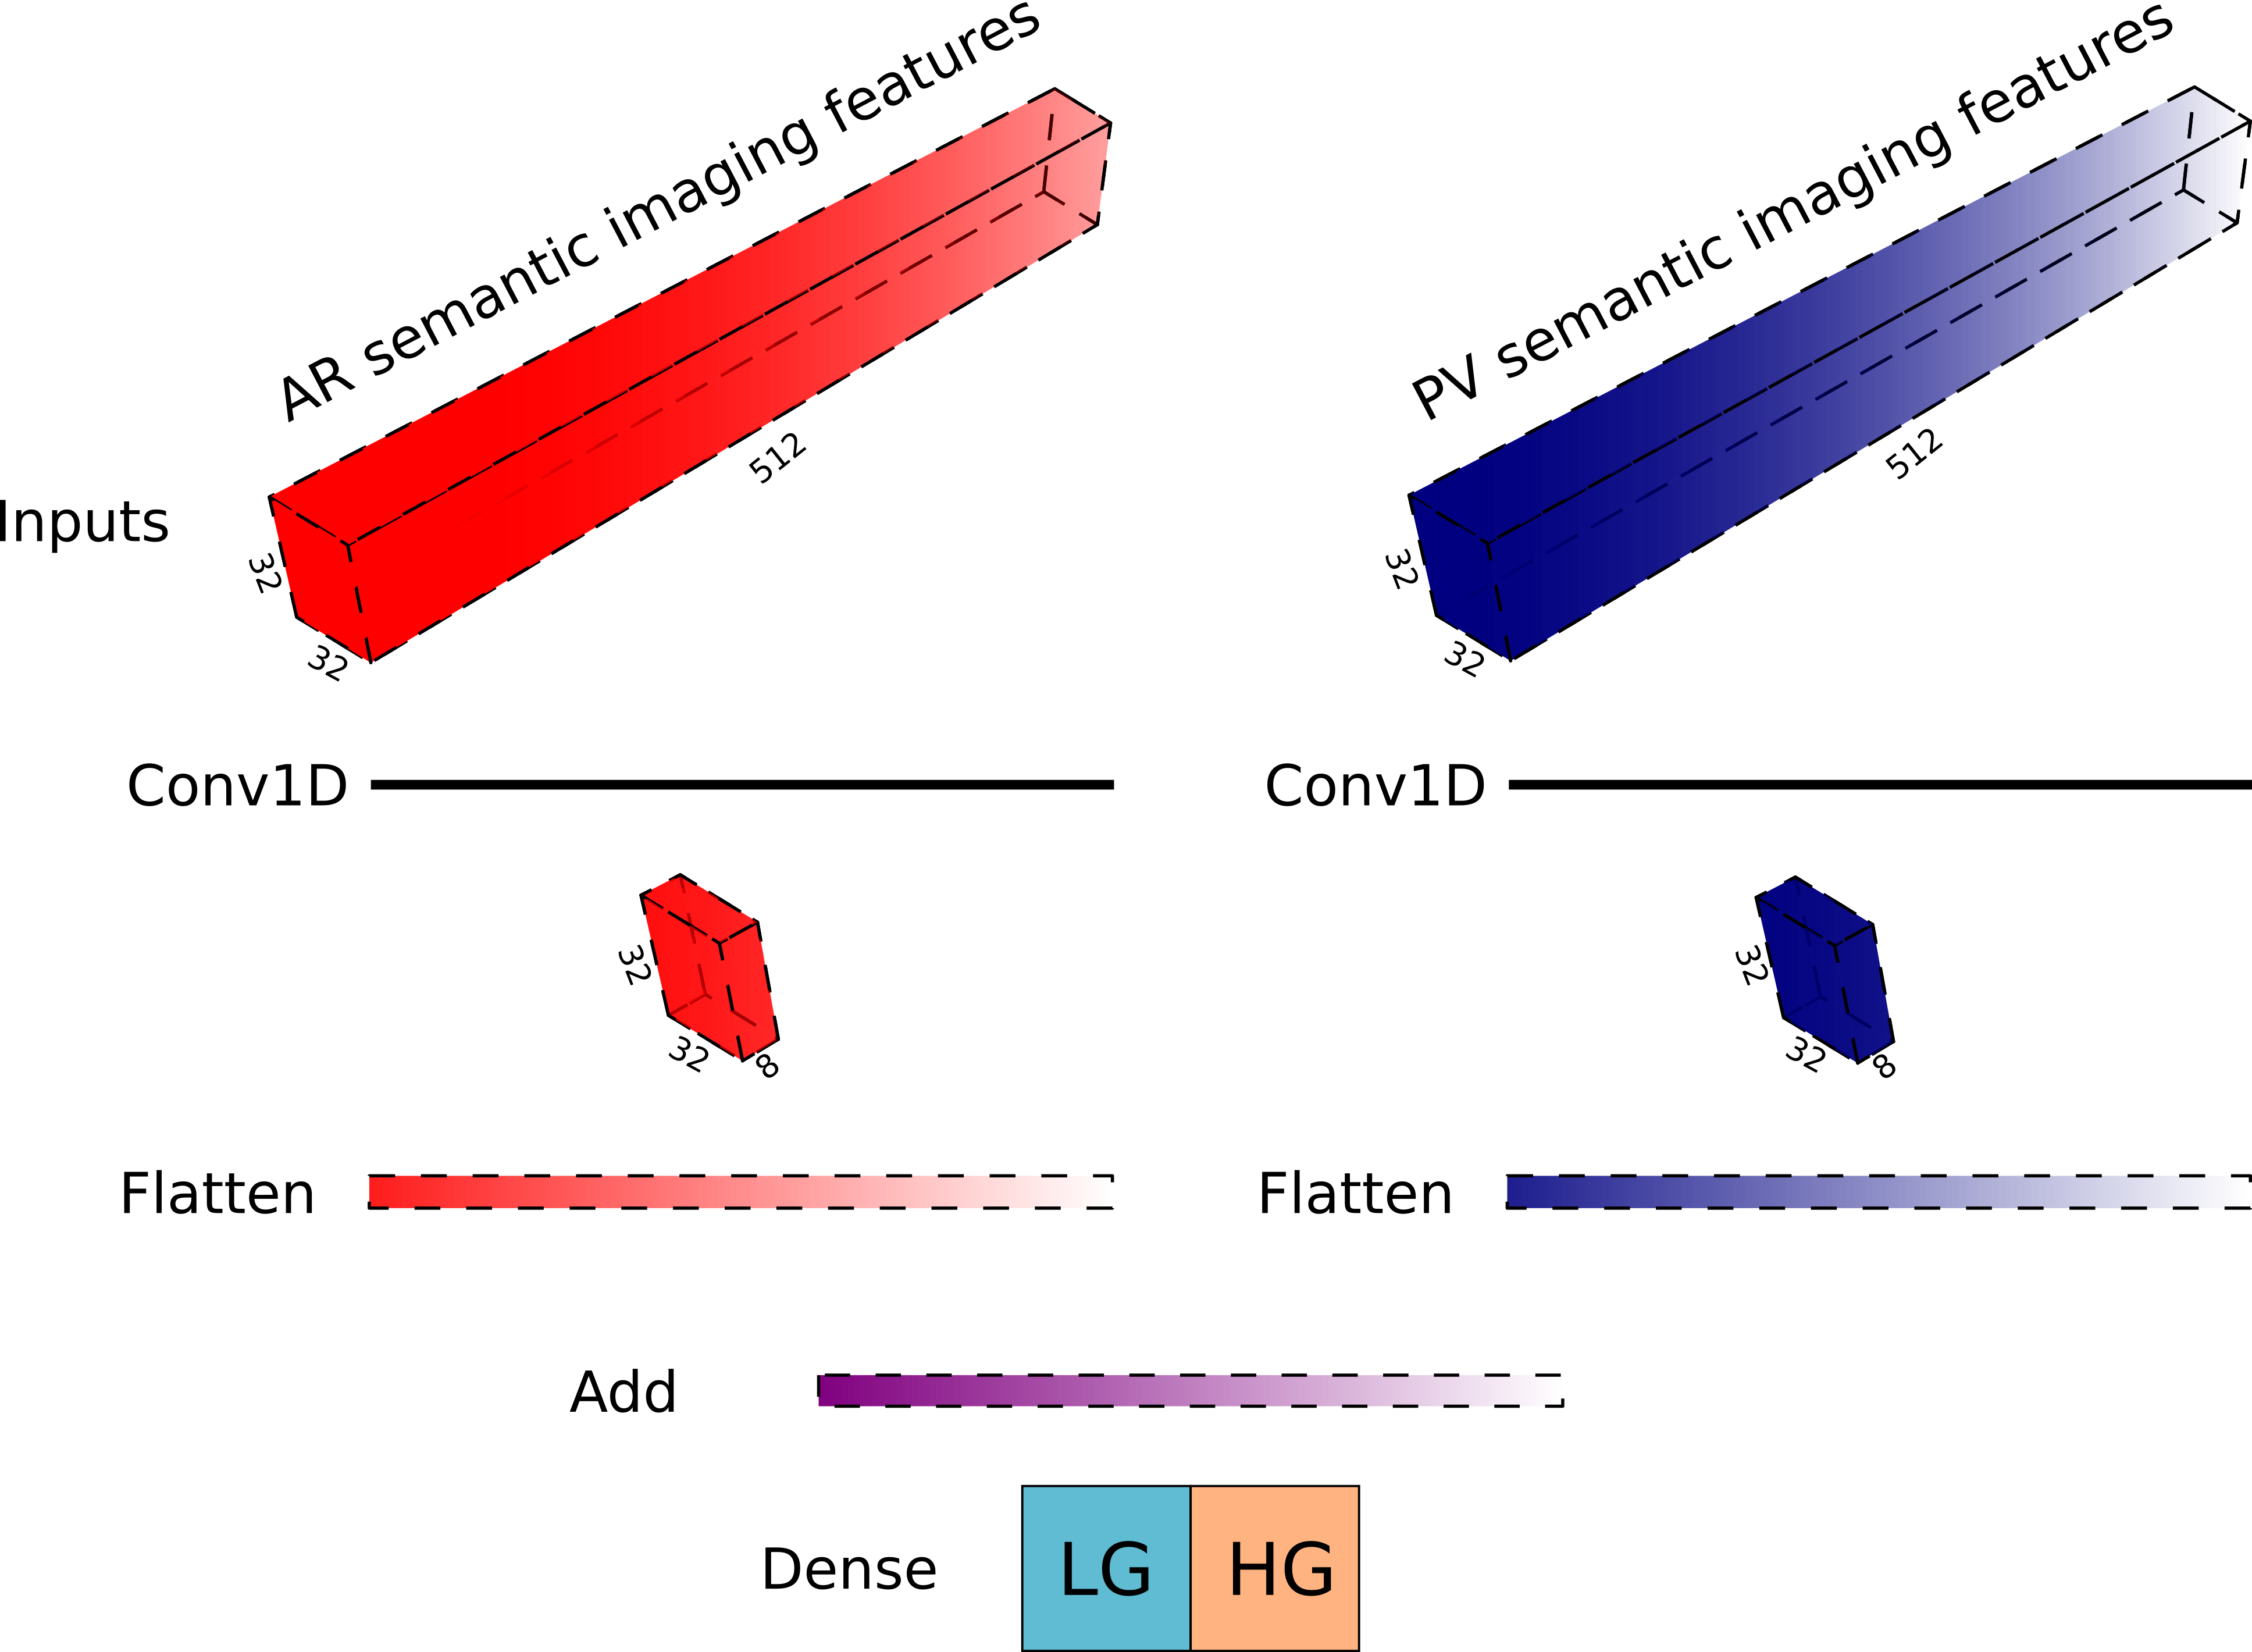
\includegraphics[width=0.9\linewidth]{../HistologicalGradePrediction/images/gradpredictionArchitecture}
\caption{Slice-wise histological grade prediction using both \ac{ar} and \ac{pv} retained semantic imaging features}
\label{fig:gradpredictionArchitecture}
\end{figure}



The architecture depicted in the figure \ref{fig:gradpredictionArchitecture} works as a dimensionality
reduction algorithm, where the first 1D convolutional layers are dedicated to
reduce the number of features initially present ($ 32\times32\times512 $). The
dimensionality reduction step is performed for each phase separately,
before the remaining features are combined (simple addition in the
features space).
A final dense layer takes the remaining features as input and computes
the probability of belonging to each class thanks to a softmax activation
function (LG vs HG).

When training the network, we decided to consider that each
centrally-located tumor slice of a given patient will have a higher
probability of exhibiting the highest grade, which in this case
corresponds to the observed patient-wise grade (ES1954 histological grading system \cite{EdmondsonHA1954}).

Knowing the composition of \textbf{\lmttfont{TCIA-dB}} (9 high grade patients vs 9 low
grade ones), we performed a 9-fold CV training, so that each patient is
at least present once in the testing set, and so that the training and
the test sets contains both the same number of patients per
class (7 patients from each class in the training set and 1 patient from
each class in the testing set).

After testing several combinations for the hyperparameters, we
fixed the number of retained features to 8 as depicted in the
figure \ref{fig:gradpredictionArchitecture} (meaning that after the features dimensionality reduction,
we obtained a $ 32\times32\times8 $ cube per phase), and we considered a 2cm volume
(corresponding to 8 centrally located slices with a 2.5mm spacing) when
training/testing our architecture.

With our CV-training, we were able to correctly predict the patient-wise
histological grade of 15 patients among 18, as detailed in the table \ref{tab:confusion_matrix} (a patient is considered as being correctly predicted
when at least half of the retained slices were annotated with the
correct \ac{gt} class).
When considering a slice-wise prediction, we were able to correctly
predict \textbf{\textasciitilde{}74\%} of the slices.\\
\renewcommand{\arraystretch}{2}
\begin{table}[!htp]\centering
\caption{Confusion matrix regarding the patient-wise  histological grade prediction}\label{tab:confusion_matrix}
\begin{tabular}{l|l|c|c|c}
\multicolumn{2}{c}{}&\multicolumn{2}{c}{\textbf{True grade}}&\\
\cline{3-4}
\multicolumn{2}{c|}{}&LG&HG&\multicolumn{1}{c}{\textit{Total}}\\
\cline{2-4}
\multirow{2}{*}{\textbf{Predicted grade}}& LG & \textbf{7} & 1 & \textbf{8}\\
\cline{2-4}
& HG & 2 & 8 & 10 \\
\cline{2-4}
\multicolumn{1}{c}{} & \multicolumn{1}{c}{\textit{Total}} & \multicolumn{1}{c}{9} & \multicolumn{1}{c}{9} & \multicolumn{1}{c}{18}\\
\end{tabular}
\end{table}
\renewcommand{\arraystretch}{5}
Those results provided a more detailed prediction than the one
consisting of a single patient-wise classification. Being able to
compute the histological grade locally (here in a slice-wise fashion)
allows us to visually focus on the heterogeneous regions that are
crucial when needing to establish a diagnosis. Our pipeline can also
provide a map of the best biopsy sites that will further be necessary in
the clinical practice to either evaluate the progression of the disease
or its prognosis.\\
We successfully proved that multiphase images incorporated in a cascaded architecture corresponds to the best combination when performing semantic segmentation of liver and its tumors. Moreover, our preliminary results proved that imaging features extracted from our cascaded multiphase segmentation architecture were relevant enough to be incorporated in a deep radiomics pipeline for the histological grade prediction. 
Our semantic segmentation results outperformed those reported on the same database using an ensemble classifier and requiring expert interactions during the segmentation process.
Our histological grade prediction results were on par with the ones reported by the only study performing histological grade prediction but using a different dataset composed of MR images and using manually drawn regions of interest.\\
In the following section we present the different axes of improvement to improve the present work.

